%%%%%%%%%%%%%%%%%%%%%%%%%%%%%%%%%%%%%%%%%%%%%%%%%%%%%%%%%%%%%%%%%%%%
%% I, the copyright holder of this work, release this work into the
%% public domain. This applies worldwide. In some countries this may
%% not be legally possible; if so: I grant anyone the right to use
%% this work for any purpose, without any conditions, unless such
%% conditions are required by law.
%%%%%%%%%%%%%%%%%%%%%%%%%%%%%%%%%%%%%%%%%%%%%%%%%%%%%%%%%%%%%%%%%%%%

\documentclass{beamer}
\usetheme[faculty=fi]{fibeamer}
\usepackage[utf8]{inputenc}
\usepackage[
   main=english, %% By using `czech` or `slovak` as the main locale
                        %% instead of `english`, you can typeset the
                        %% presentation in either Czech or Slovak,
                        %% respectively.
   czech, slovak, greek %% The additional keys allow foreign texts to be
]{babel}            %% typeset as follows:


\usepackage{mathtools}
\usepackage{amsmath}
\usepackage{multirow} % to have tables with multi rows

%% These macros specify information about the presentation
\title{
   Microbial communities through the lens of high throughput sequencing, data integration and metabolic networks analysis
}

\subtitle{
   developing computational approaches to better understand 
   % questions of \textit{what - where - who} about the role of microbes in biogeochemical cycles
   microbial assemblages
}

\author{
   Haris Zafeiropoulos \\ 
   \scriptsize PhD candidate
}


% \newline
% \scriptsize \textbf{Workshop:} Circular Bioeconomy and sustainable development \\
% \scriptsize \textit{2022.06.09}



%% These additional packages are used within the document:
\usepackage{ragged2e}                                       % `\justifying` text
\usepackage{booktabs}                                       % Tables
\usepackage{tabularx}
\usepackage{tikz}                                           % Diagrams
\usetikzlibrary{calc, shapes, backgrounds}
\usepackage{amsmath, amssymb}
\usepackage{url}                                            % `\url`s
\usepackage{listings}                                       % Code listings
\usepackage{setspace}
\usepackage[absolute,overlay]{textpos}                      

\setbeamertemplate{caption}{\raggedright\insertcaption\par}


\frenchspacing

\begin{document}

   \shorthandoff{-}
   \frame[c]{
      \maketitle
   }

   % -------------------------
   %  TOC 
   % -------------------------
   
   % Print an outline at the beginning of sections
   \AtBeginSection[]{
      \begin{frame}<beamer>
         \tableofcontents[currentsection]
      \end{frame}
   }

   % -------------------------------------- mute for the phd defense presentation ----------------------------
   \if 0
   % BEBIN A SECTION ABOUT ME
   \begin{darkframes}
      \section{My short story}
   \end{darkframes}

   % OLYMPIA TIMES
   \begin{frame}

      \frametitle{
         My story starts at a small but quite a nice place
         }
      \framesubtitle{Ancient Olympia}

      \begin{tikzpicture}
         \node[anchor=west, xshift=-15pt, yshift=45pt]               
         at (current page.west) {
            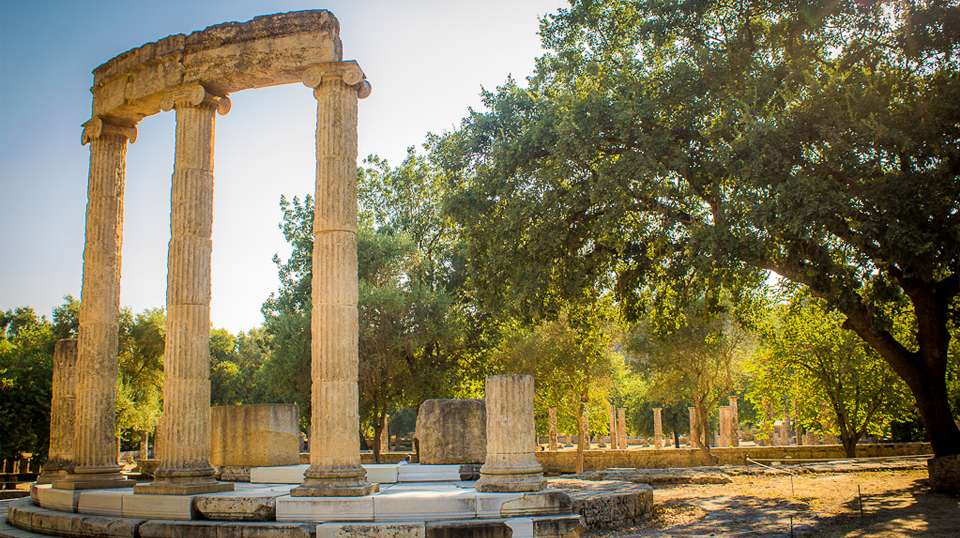
\includegraphics[width=55mm]{
               resources/olympia.jpg}
         };

         \node[anchor=east, xshift=-52pt, yshift=45pt]               
         at (current page.east) {
            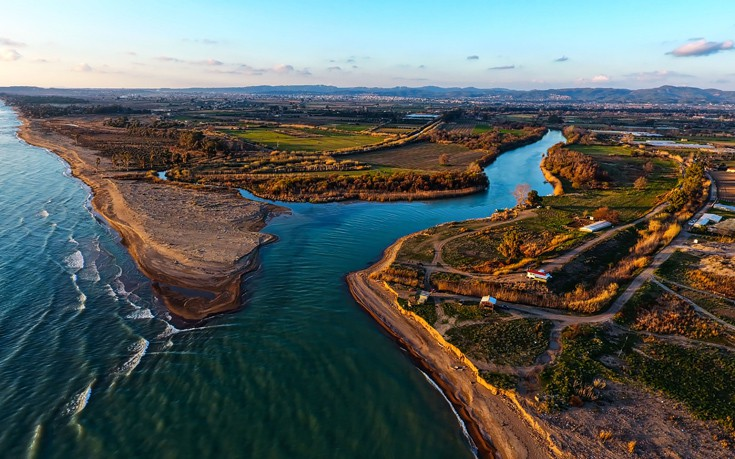
\includegraphics[width=55mm]{
               resources/alfios.jpg}
         };

      \end{tikzpicture}

      \begin{textblock*}{10cm}(1.0cm, 8.0cm)
         \small Great times with a lot of basketball and even more \textit{hows} and \textit{whys}
      \end{textblock*}

   \end{frame}

   % EKPA TIMES 
   \begin{frame}
      \frametitle{.. moves in Athens}
      \framesubtitle{Biology Department, National \& Kapodestrian University}
      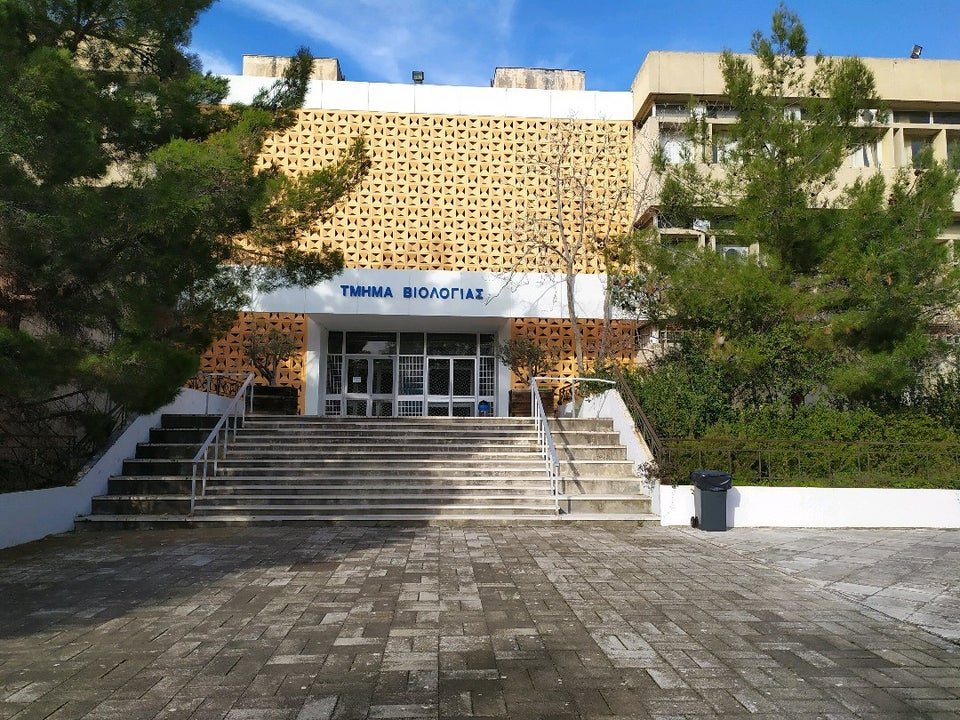
\includegraphics[width=60mm]{resources/biol_depart_ekpa.jpg} 
      \begin{textblock*}{5cm}(7.5cm, 5.0cm)
         \small Thesis on the morphology, morphometry and anatomy of species of the genus \textit{Pseudamnicola} in Greece
      \end{textblock*}
   \end{frame}

   % UoC TIMES 
   \begin{frame}

      \frametitle{.. and then to a "horrible" place called Crete}
      \framesubtitle{
         Medical School (MSc), Biology department (PhD) of UoC, \\
         Hellenic Centre for Marine Research
         }

      \begin{tikzpicture}

         \node[anchor=east, xshift=-130pt, yshift=30pt]               
         at (current page.east) {
            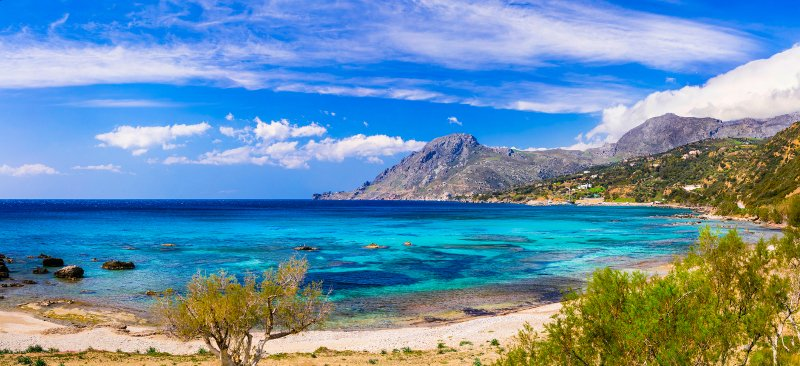
\includegraphics[width=60mm]{
               resources/plakias.jpg}
         };

         \node[anchor=east, 
         xshift=20pt]
         at (current page.east) {
            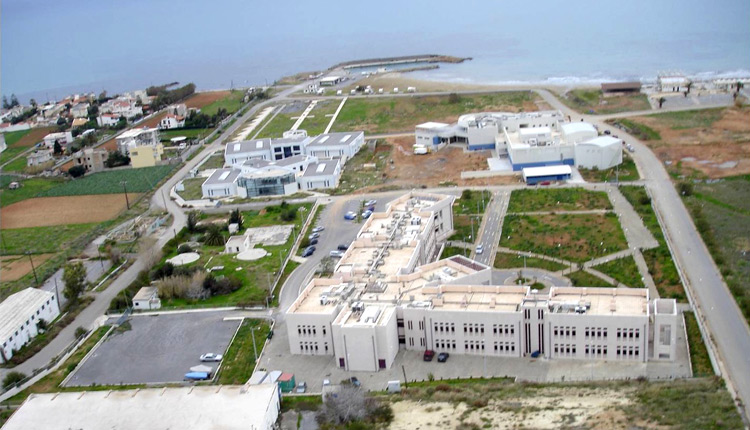
\includegraphics[width=50mm]{
               resources/hcmr.jpg}
         };

      \end{tikzpicture}

      % TEXT BLOCK
      \begin{textblock*}{10cm}(1.0cm, 8.0cm)

         \small MSc thesis on eDNA metabarcoding for biodiversity assessment: 
         Algorithm design and bioinformatics analysis pipeline implementation
         
      \end{textblock*}


   \end{frame}
   \fi
   % -------------------------------------- mute for the phd defense presentation ----------------------------


   % -------------------------
   % CHANGE THE CHAPTER SLIDE: MICROBIAL ECOLOGY INTRO
   % -------------------------
   \begin{darkframes}
      \section{
         % \textbf{Chapter 1}: 
         Introduction
      }
   \end{darkframes}

   % INTRO
   \begin{frame}

      \frametitle{Microbial ecology \& biogeochemical cycles}
      \framesubtitle{a corner-stone for life on earth}

      \begin{singlespace}
         \begin{tikzpicture}[overlay,remember picture]
            \node[anchor=west, xshift=30pt,yshift=-165pt]
               at (current page.north west) {
                  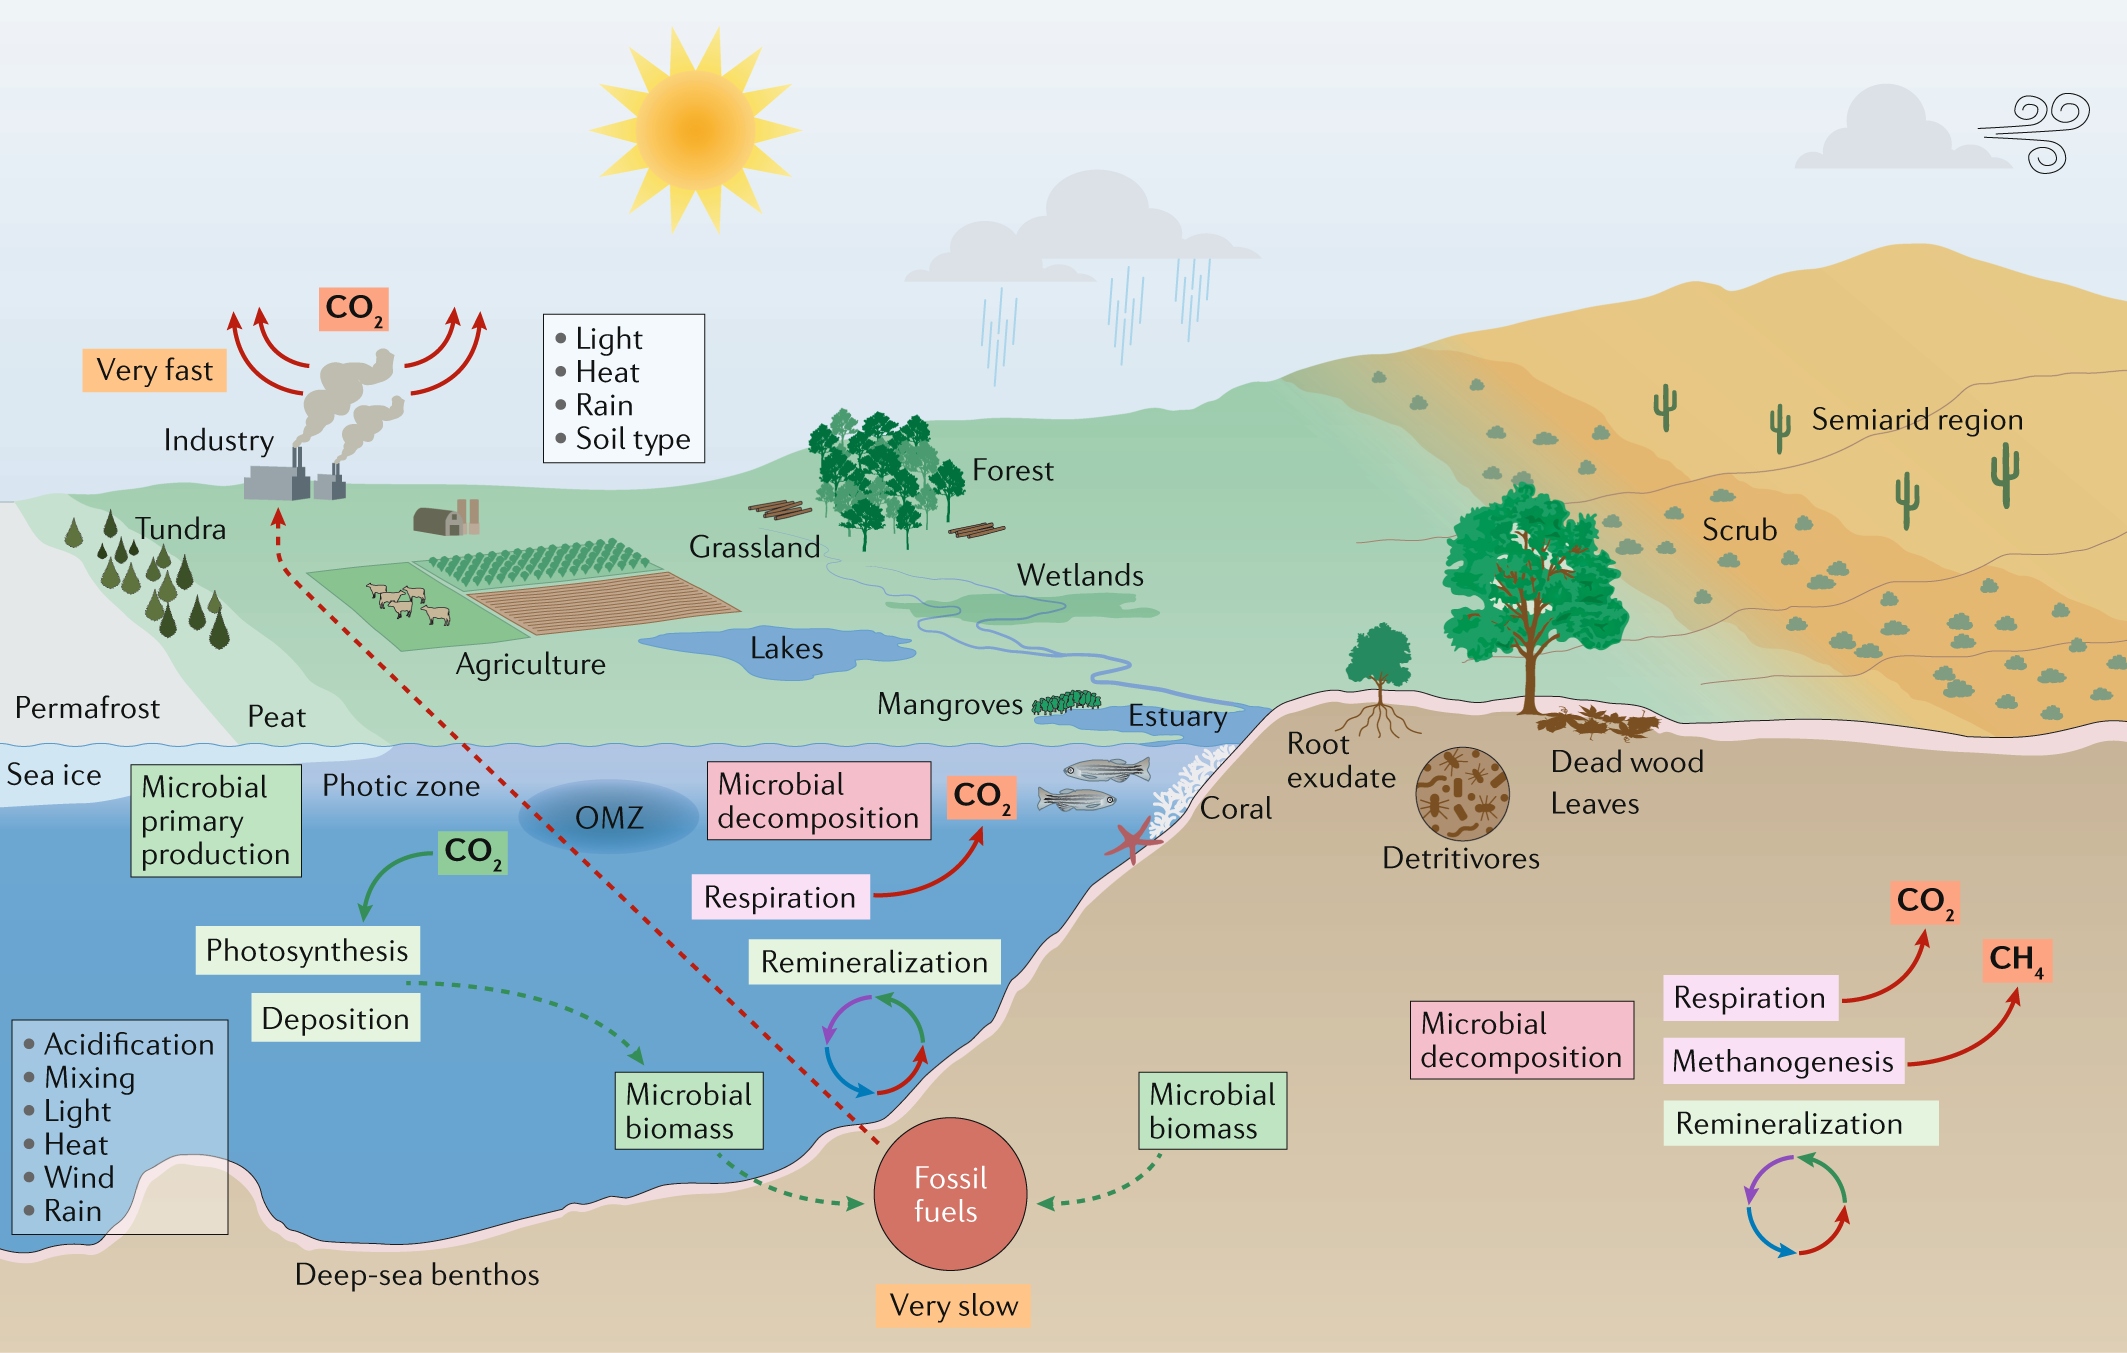
\includegraphics[width=75mm]{resources/ecosystem_functioning.png}
                  
               };
               \node[anchor=west, xshift=33pt,yshift=-240pt]
               at (current page.north west) {
                  \scriptsize Figure from: Nature Reviews Microbiology 17.9 (2019): 569-586.
                  
               };

            \node[anchor=west, xshift=230pt,yshift=-185pt]
              at (current page.north west) {

               \begin{textblock*}{3cm}(9.0cm, 4.0cm)
                  \centering

                  \begin{itemize}
                     \item composition 
                     \item functions 
                     \item interactions 
                  \end{itemize}
                  
                  \hrulefill

                  \begin{itemize}
                     \item[$\rightarrow$] power biogeochemical cycling
                  \end{itemize}

               \end{textblock*}
            };

            \node[anchor=west, xshift=130pt, yshift=-35pt]
               at (current page.north) {
                  
\includegraphics[width=15mm]{resources/chapter1.png}
                  
               };

         \end{tikzpicture}
      \end{singlespace}

   \end{frame}

   % MAIN QUESTIONS 
   \begin{frame}
      \frametitle{Main questions regarding a microbial community}
      \framesubtitle{for a deeper understanding of such assemblages}
      \begin{singlespace}


         \begin{columns}[onlytextwidth]
            
            \column{.33\textwidth}

               \begin{center}

                  Community \\ structure   \\ \textbf{\textit{who}}  

                  \hrulefill

                  \scriptsize \textit{eveyrone is everywhere}

               \end{center}


            \column{.33\textwidth}

               \begin{center}

                  Functional \\ potential \\ \textbf{\textit{what}}

                  \hrulefill

                  \scriptsize \textit{zero-sum game}

               \end{center}

            \column{.33\textwidth}

               \begin{center}

                  Microbial \\ interactions \\ \textbf{\textit{why / how}}

                  \hrulefill

                  \scriptsize \textit{the entagnled bank}

               \end{center}
      

         \end{columns}

         % RELATED CHAPTER
         \begin{tikzpicture}[overlay,remember picture]
            \node[anchor=west, xshift=130pt, yshift=-35pt]
            at (current page.north) {
               
\includegraphics[width=15mm]{resources/chapter1.png}
            };
         \end{tikzpicture}


      \end{singlespace}

   \end{frame}

   % REVERSE ECOLOGY
   \begin{frame}

      \frametitle{Reverse ecology}
      \framesubtitle{transforming ecology into a high-throughput field}

      \begin{singlespace}
         \begin{tikzpicture}[overlay,remember picture]
            \node[anchor=west, xshift=30pt,yshift=-150pt]
               at (current page.north west) {
                  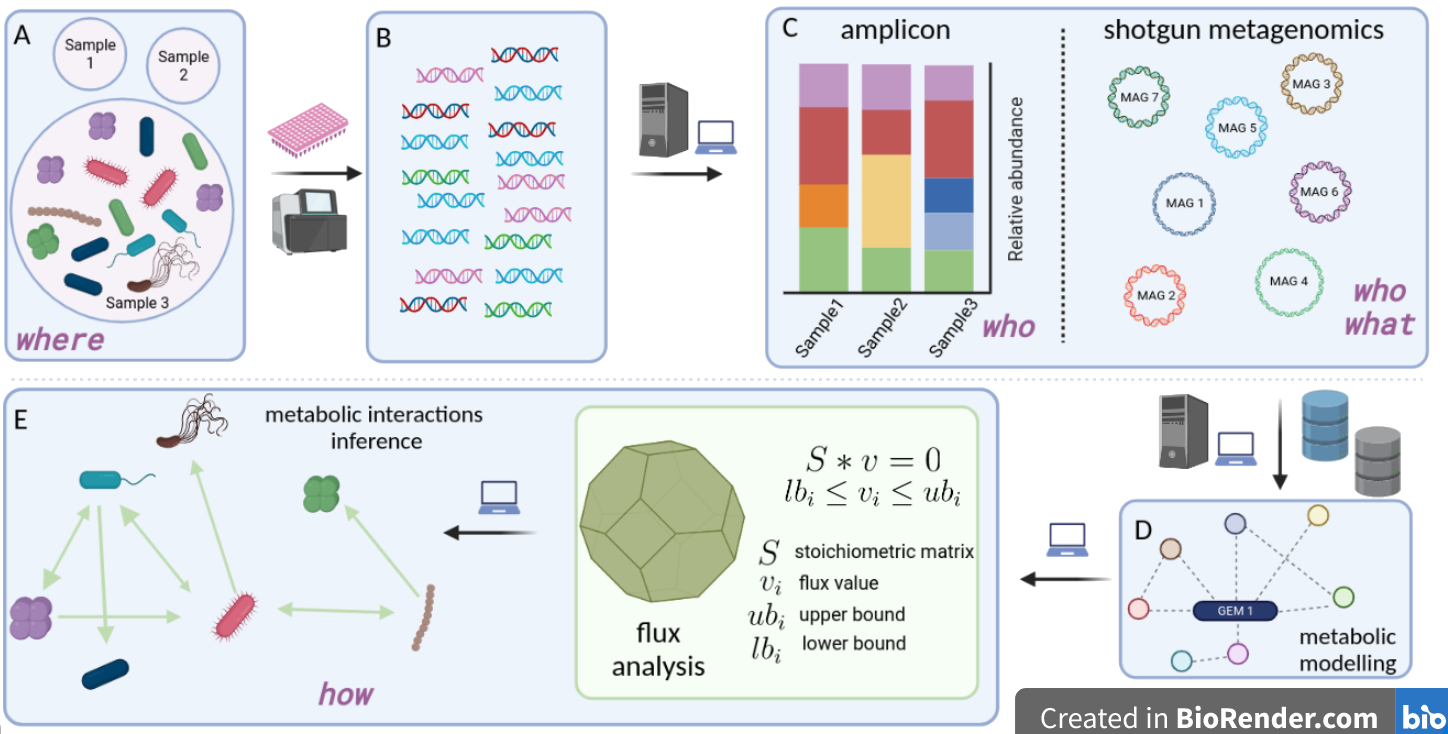
\includegraphics[width=75mm]{resources/reverse_ecology_transp.png}
                  
               };
            \node[anchor=east, xshift=30pt,yshift=-165pt]
              at (current page.north east){
               \begin{textblock*}{3cm}(9.0cm, 3.5cm)
                  \small	
                  community ecology studies with no \textit{a priori} assumptions about the organisms under consideration \\
                  \small	
                  by exploiting advances in systems biology and genomic metabolic modeling
               \end{textblock*}
         
              };

         % RELATED CHAPTER
            \node[anchor=west, xshift=130pt, yshift=-35pt]
            at (current page.north) {
               
\includegraphics[width=15mm]{resources/chapter1.png}
            };

         \end{tikzpicture}
      \end{singlespace}

   \end{frame}

   % CHALLENGES
   \begin{frame}
      \frametitle{From raw reads to community analysis}
      \framesubtitle{not a straight-forward way}

      \begin{singlespace}
         \begin{tikzpicture}[overlay,remember picture]
            \node[anchor=east, xshift=-5pt, yshift=-150pt]
               at (current page.north east) {
                  
\includegraphics[width=70mm]{resources/challenges.jpeg}
                  
               };
            \node[anchor=west]
              at (current page.north west){
               \begin{textblock*}{5cm}(0.8cm, 3.5cm)
                  \footnotesize
                  \begin{itemize}
                     \item biology-oriented issues           % genetic variance, broken pieces, alive and dead 
                     \item techonology-oriented issues       % resolytion, primets, pcr biases 
                     \item computing requirements            % storage, memory, algorithm 
                     \item data and metadata \\ accessiblity    % standards, ontologies, data integration apps 
                  \end{itemize}

               \end{textblock*}
         
              };

            % RELATED CHAPTER
            \node[anchor=west, xshift=130pt, yshift=-35pt]
            at (current page.north) {
               
\includegraphics[width=15mm]{resources/chapter1.png}
            };
         
         \end{tikzpicture}
      \end{singlespace}
   \end{frame}

   % AIM OF THIS PHD
   \begin{frame}
      \frametitle{Aims and objectives}
      \begin{itemize}
         \item \small to enhance the analysis of microbiome data by building algorithms and software
         that address limitations and on-going computational challenges
         \bigskip
         \item  to exploit state-of-the-art methods to identify taxa and functions that play a key
         part in microbial community assemblages in hypersaline sediments
      \end{itemize}

      % RELATED CHAPTER
      \begin{tikzpicture}[overlay,remember picture]
         \node[anchor=west, xshift=130pt, yshift=-35pt]
         at (current page.north) {
            
\includegraphics[width=15mm]{resources/chapter1.png}
         };
      \end{tikzpicture}
   \end{frame}


   % -------------------------
   % CHANGE THE CHAPTER SLIDE: HIGH THROUGHPUT SEQUENCING INTRO
   % -------------------------


   \begin{darkframes}
      \section{
      % \textbf{Chapter 2}: 
      Software development to support HTS-oriented methods for microbial diversity assessment
      }
   \end{darkframes}

   % MARKER GENES - BIOINFO STEPS
   \begin{frame}
      
      \frametitle{eDNA metabarcoding}
      \framesubtitle{for biodiversity assessment}
      \begin{singlespace}


         \begin{columns}[onlytextwidth]

            \column{.5\textwidth}

               \textbf{Marker genes} \\ 

               \begin{enumerate}
                  \item \textbf{16S rRNA:} Bacteria, Archaea
                  \item \textbf{12S rRNA:} Vertebrates
                  \item \textbf{18S rRNA:} Small eukaryotes, Metazoa
                  \item \textbf{ITS:} Fungi
                  \item \textbf{COI:} Eukaryotes
                  \item \textbf{\textit{rbcl}:} Plants
                  \item \textbf{\textit{dsrb}:} Bacteria, Archaea
                  \item ...
               \end{enumerate}

            \column{.45\textwidth}

               \textbf{Methodology}

               \begin{figure}
                  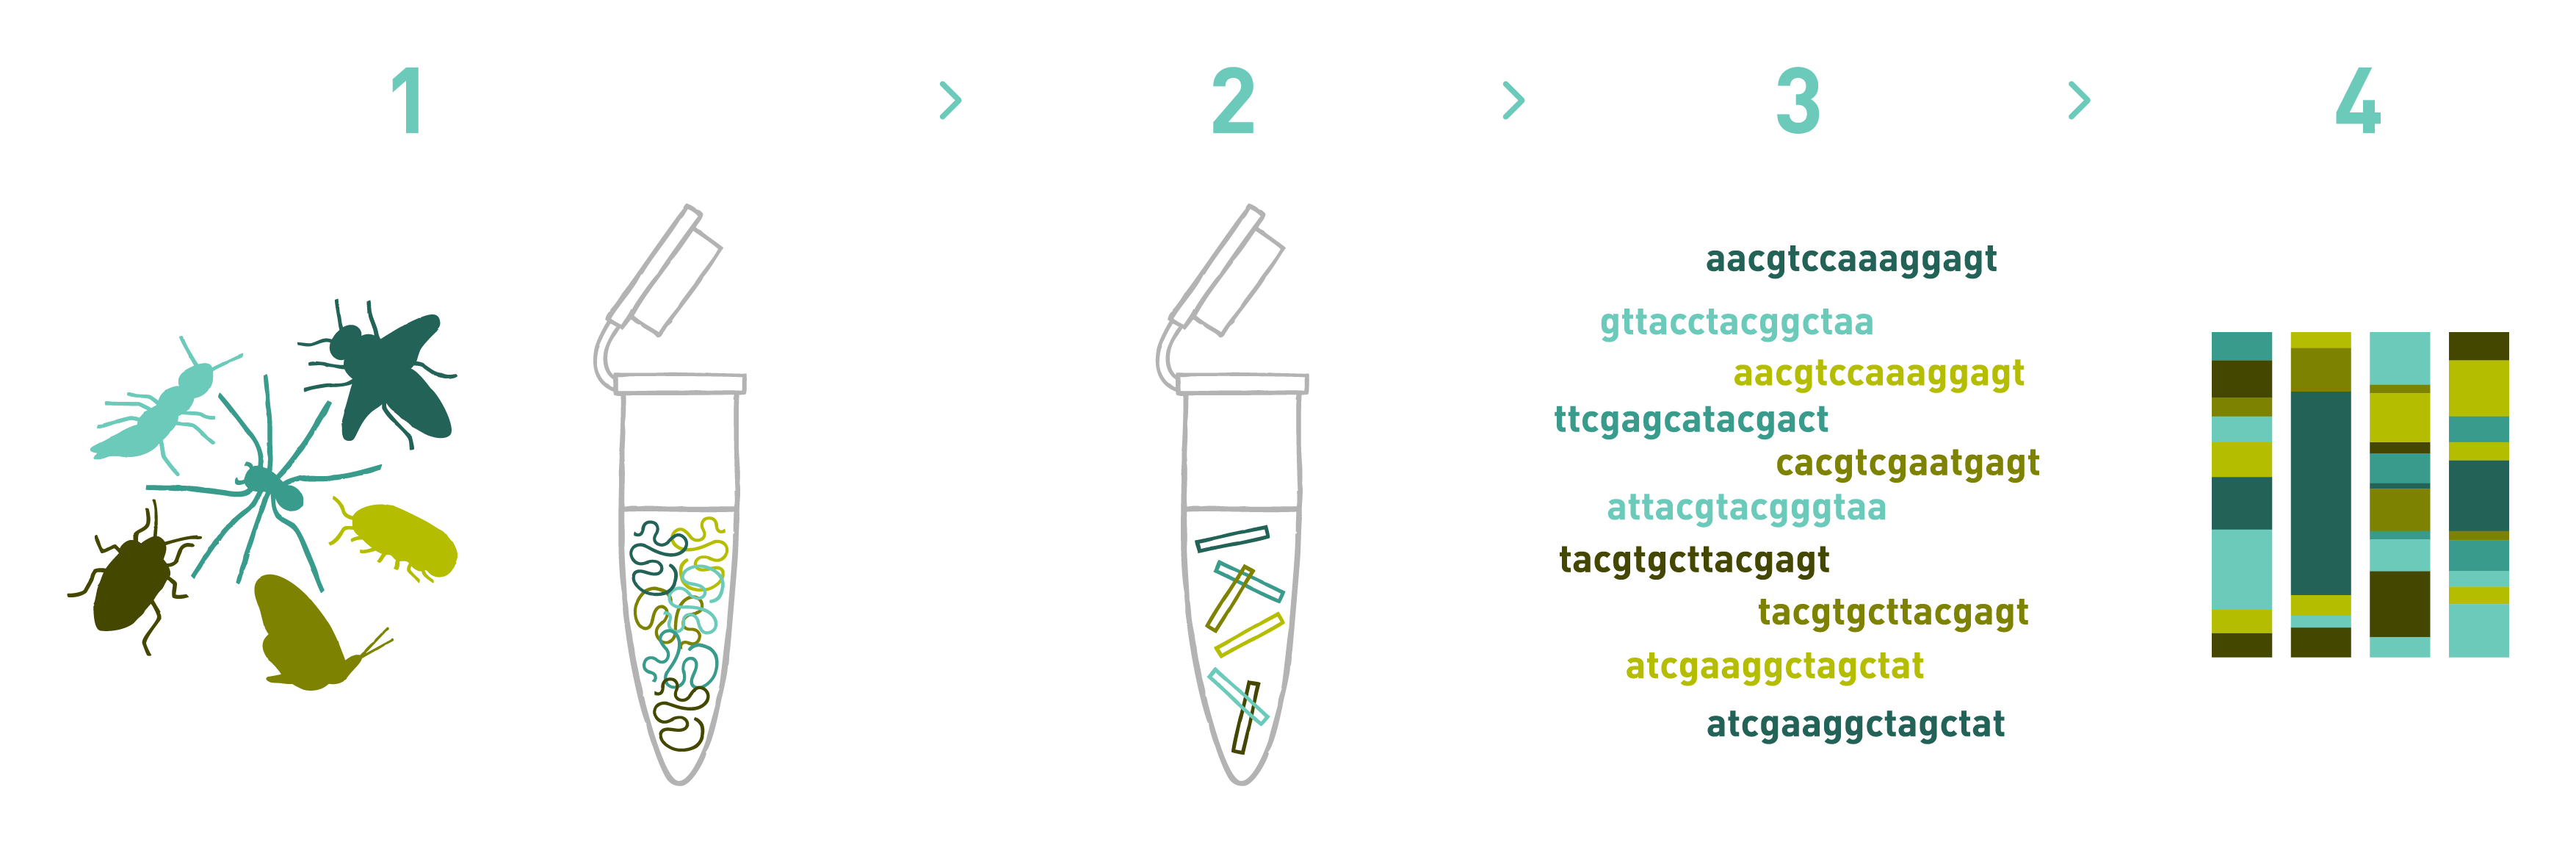
\includegraphics[width=55mm]{resources/metabarcoding-steps.png}
               \end{figure}

               \begin{itemize}
                  \item Sampling
                  \item Extraction
                  \item Bioinformatics
                  \item Biodiversity analysis
               \end{itemize}
               

         \end{columns}

         % RELATED CHAPTER
         \begin{tikzpicture}[overlay,remember picture]
            \node[anchor=west, xshift=130pt, yshift=-35pt]
            at (current page.north) {
               
\includegraphics[width=15mm]{resources/chapter2.png}
            };
         \end{tikzpicture}

      \end{singlespace}
   \end{frame}

   % BIOINFORMATICS CHALLENGES 
   \begin{frame}
      \frametitle{Bioinformatics challenges}
      \framesubtitle{for the analysis and the interpretation of amplicon data}

      \begin{columns}[onlytextwidth]

         \column{.5\textwidth}

            
\includegraphics[width=40mm]{resources/bioinfo_mess.png}

         \column{.5\textwidth}

            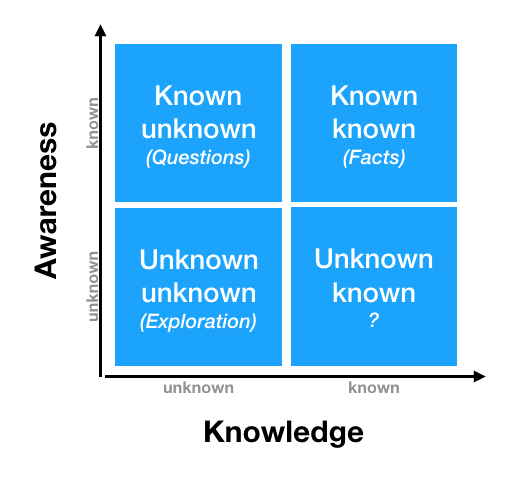
\includegraphics[width=50mm]{resources/known_unknown.png}
         
      \end{columns}


      % RELATED CHAPTER
      \begin{tikzpicture}[overlay,remember picture]
         \node[anchor=west, xshift=130pt, yshift=-35pt]
         at (current page.north) {
            
\includegraphics[width=15mm]{resources/chapter2.png}
         };
      \end{tikzpicture}

   \end{frame}

   % -------------------------
   % CHANGE SUBSECTION: PEMA 
   % -------------------------

   % PEMA SUBSECTION
   \begin{darkframes}
      \subsection{PEMA: a Pipeline for Environmental DNA Metabarcoding Analysis}
   \end{darkframes}
   
    % AIM OF STUDY
   \begin{darkframes}
      \begin{frame}
         \frametitle{PEMA: a flexible Pipeline for Environmental DNA Metabarcoding Analysis of the
         16S/18S ribosomal RNA, ITS \& COI marker genes}
         \framesubtitle{Aim of the study and contribution}

         To build an open source
         pipeline that bundles state-of-the-art bioinformatics tools for all necessary steps of
         amplicon analysis and aims to address:
         \begin{itemize}
            \item one-stop-shop for several marker genes \& approaches
            \item easy-to-set \& easy-to-use 
            \item scalable
            \item flexible
         \end{itemize}
      \end{frame}
   \end{darkframes}

   % BIOINFORMATICS TRICKS AND HINTS
   \begin{frame}
      \frametitle{Methods / Implementation}
      \framesubtitle{PEMA coding insights}

      \begin{columns}[onlytextwidth]
         
         \column{0.2\textwidth}
         
            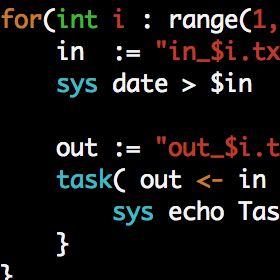
\includegraphics[width=25mm]{resources/bds.png}
            \centering
            \texttt{BigDataScript} \\
            programming language

         \column{0.4\textwidth}

            \begin{tikzpicture}[overlay,remember picture]

               \node[anchor=east, xshift=-185pt, yshift=10pt]               
                  at (current page.east) {

                     
\includegraphics[width=17mm]{resources/sing_transp.png}
                  
                  };

                  \node[anchor=east, xshift=-115pt, yshift=10pt]
                  at (current page.east) {

                     
\includegraphics[width=25mm]{resources/docker_facebook_share.png}
                  
                  };

                  \node[anchor=south, align = center, above, xshift=5, yshift=90]
                  at (current page.south) {

                     Containerization

                  };

            \end{tikzpicture}
            
         \column{0.2\textwidth}
            \begin{tikzpicture}[overlay,remember picture]

               \node[anchor=east, xshift=-20pt, yshift=10pt]               
                  at (current page.east) {

                     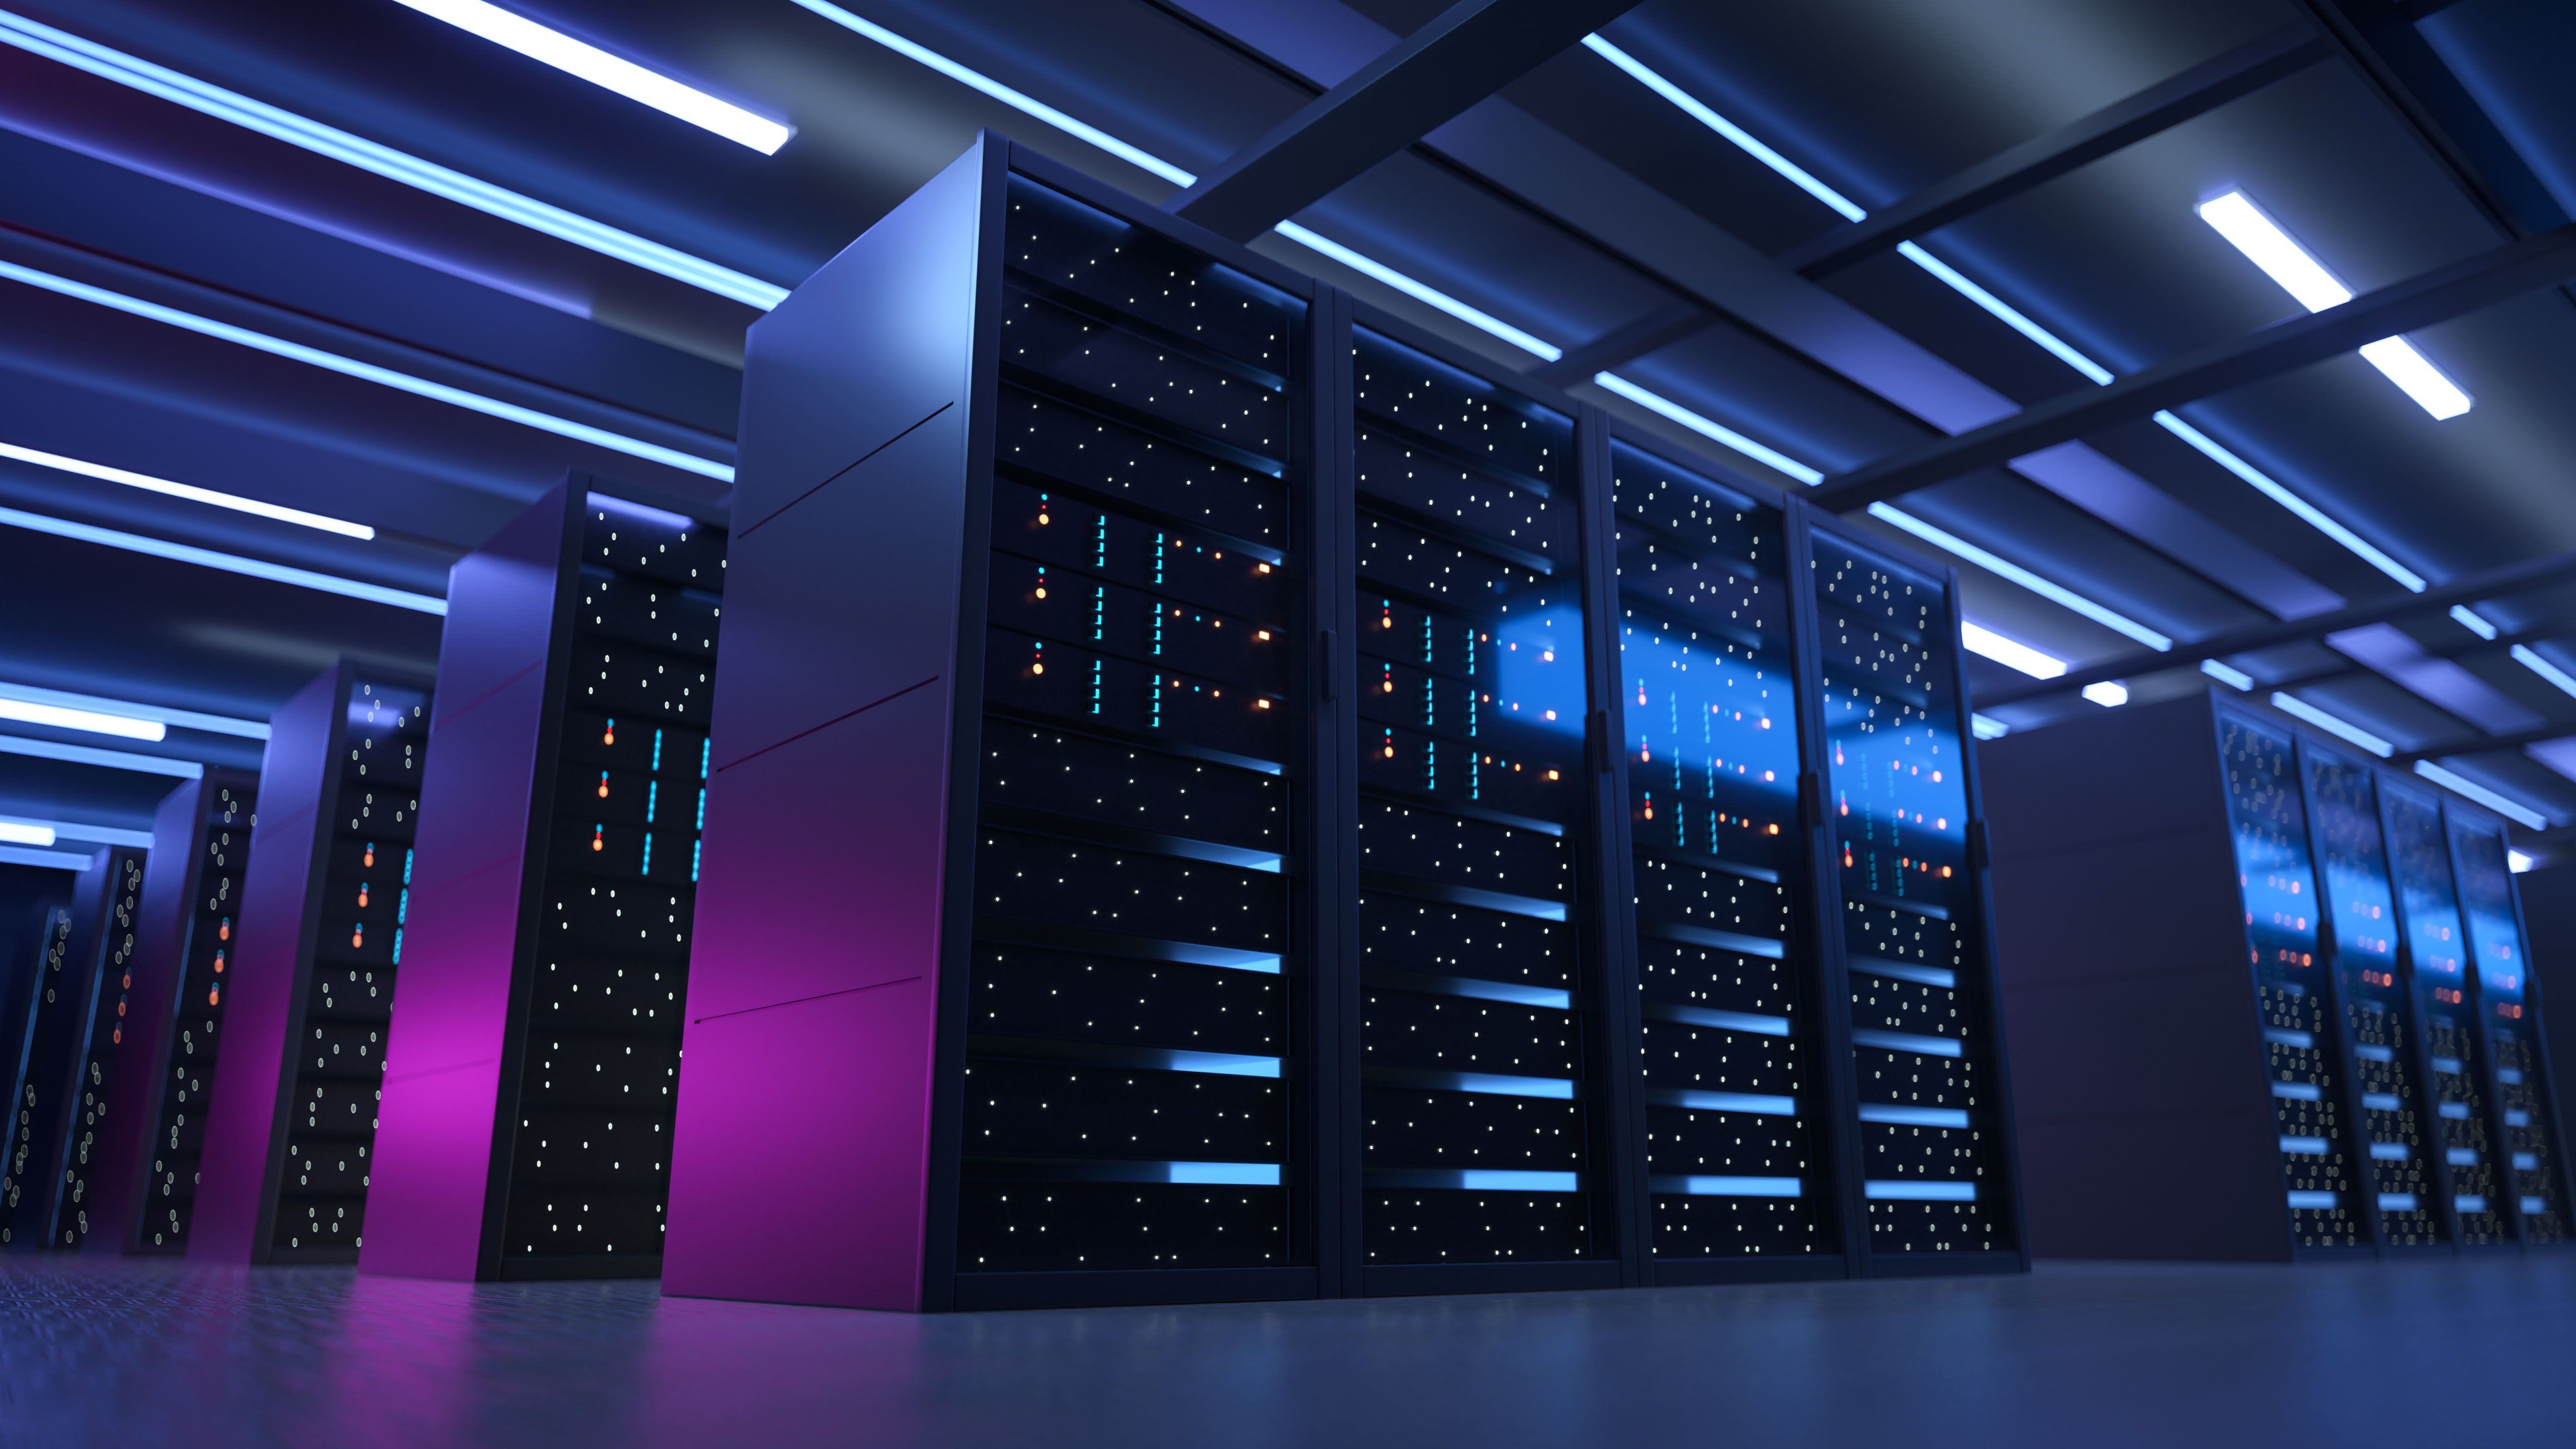
\includegraphics[width=32mm]{resources/hpc.jpg}
                  
                  };

               \node[anchor=south, align = center, above, xshift=112, yshift=80]
               at (current page.south) {

                  High performance \\
                  computing
      
               };
            \end{tikzpicture}
      \end{columns}

      % RELATED CHAPTER
      \begin{tikzpicture}[overlay,remember picture]
         \node[anchor=west, xshift=130pt, yshift=-35pt]
         at (current page.north) {
            
\includegraphics[width=15mm]{resources/chapter2.1.png}
         };
      \end{tikzpicture}

   \end{frame}

   % WORKFLOW SLIDE
   \begin{frame}
      \frametitle{Results: PEMA features}
      \framesubtitle{an overview}
      \begin{singlespace}
         \begin{tikzpicture}[overlay,remember picture]
            \node[anchor=west, xshift=30pt,yshift=-165pt]
               at (current page.north west) {
                  \includegraphics[width=104mm]{resources/pema-pema.drawio.png}
               };

         \end{tikzpicture}
      \end{singlespace}
      % RELATED CHAPTER
      \begin{tikzpicture}[overlay,remember picture]
         \node[anchor=west, xshift=130pt, yshift=-35pt]
         at (current page.north) {
            
\includegraphics[width=15mm]{resources/chapter2.1.png}
         };
      \end{tikzpicture}


   \end{frame}

   % PHYLOGENY TREE
   \begin{frame}
      \frametitle{Results: PEMA features}
      \framesubtitle{phylogeny-based taxonomy assigment for the case of 16S rRNA gene}
      \begin{singlespace}
         \begin{tikzpicture}[overlay,remember picture]
            \node[anchor=west, xshift=30pt,yshift=-165pt]
               at (current page.north west) {
                  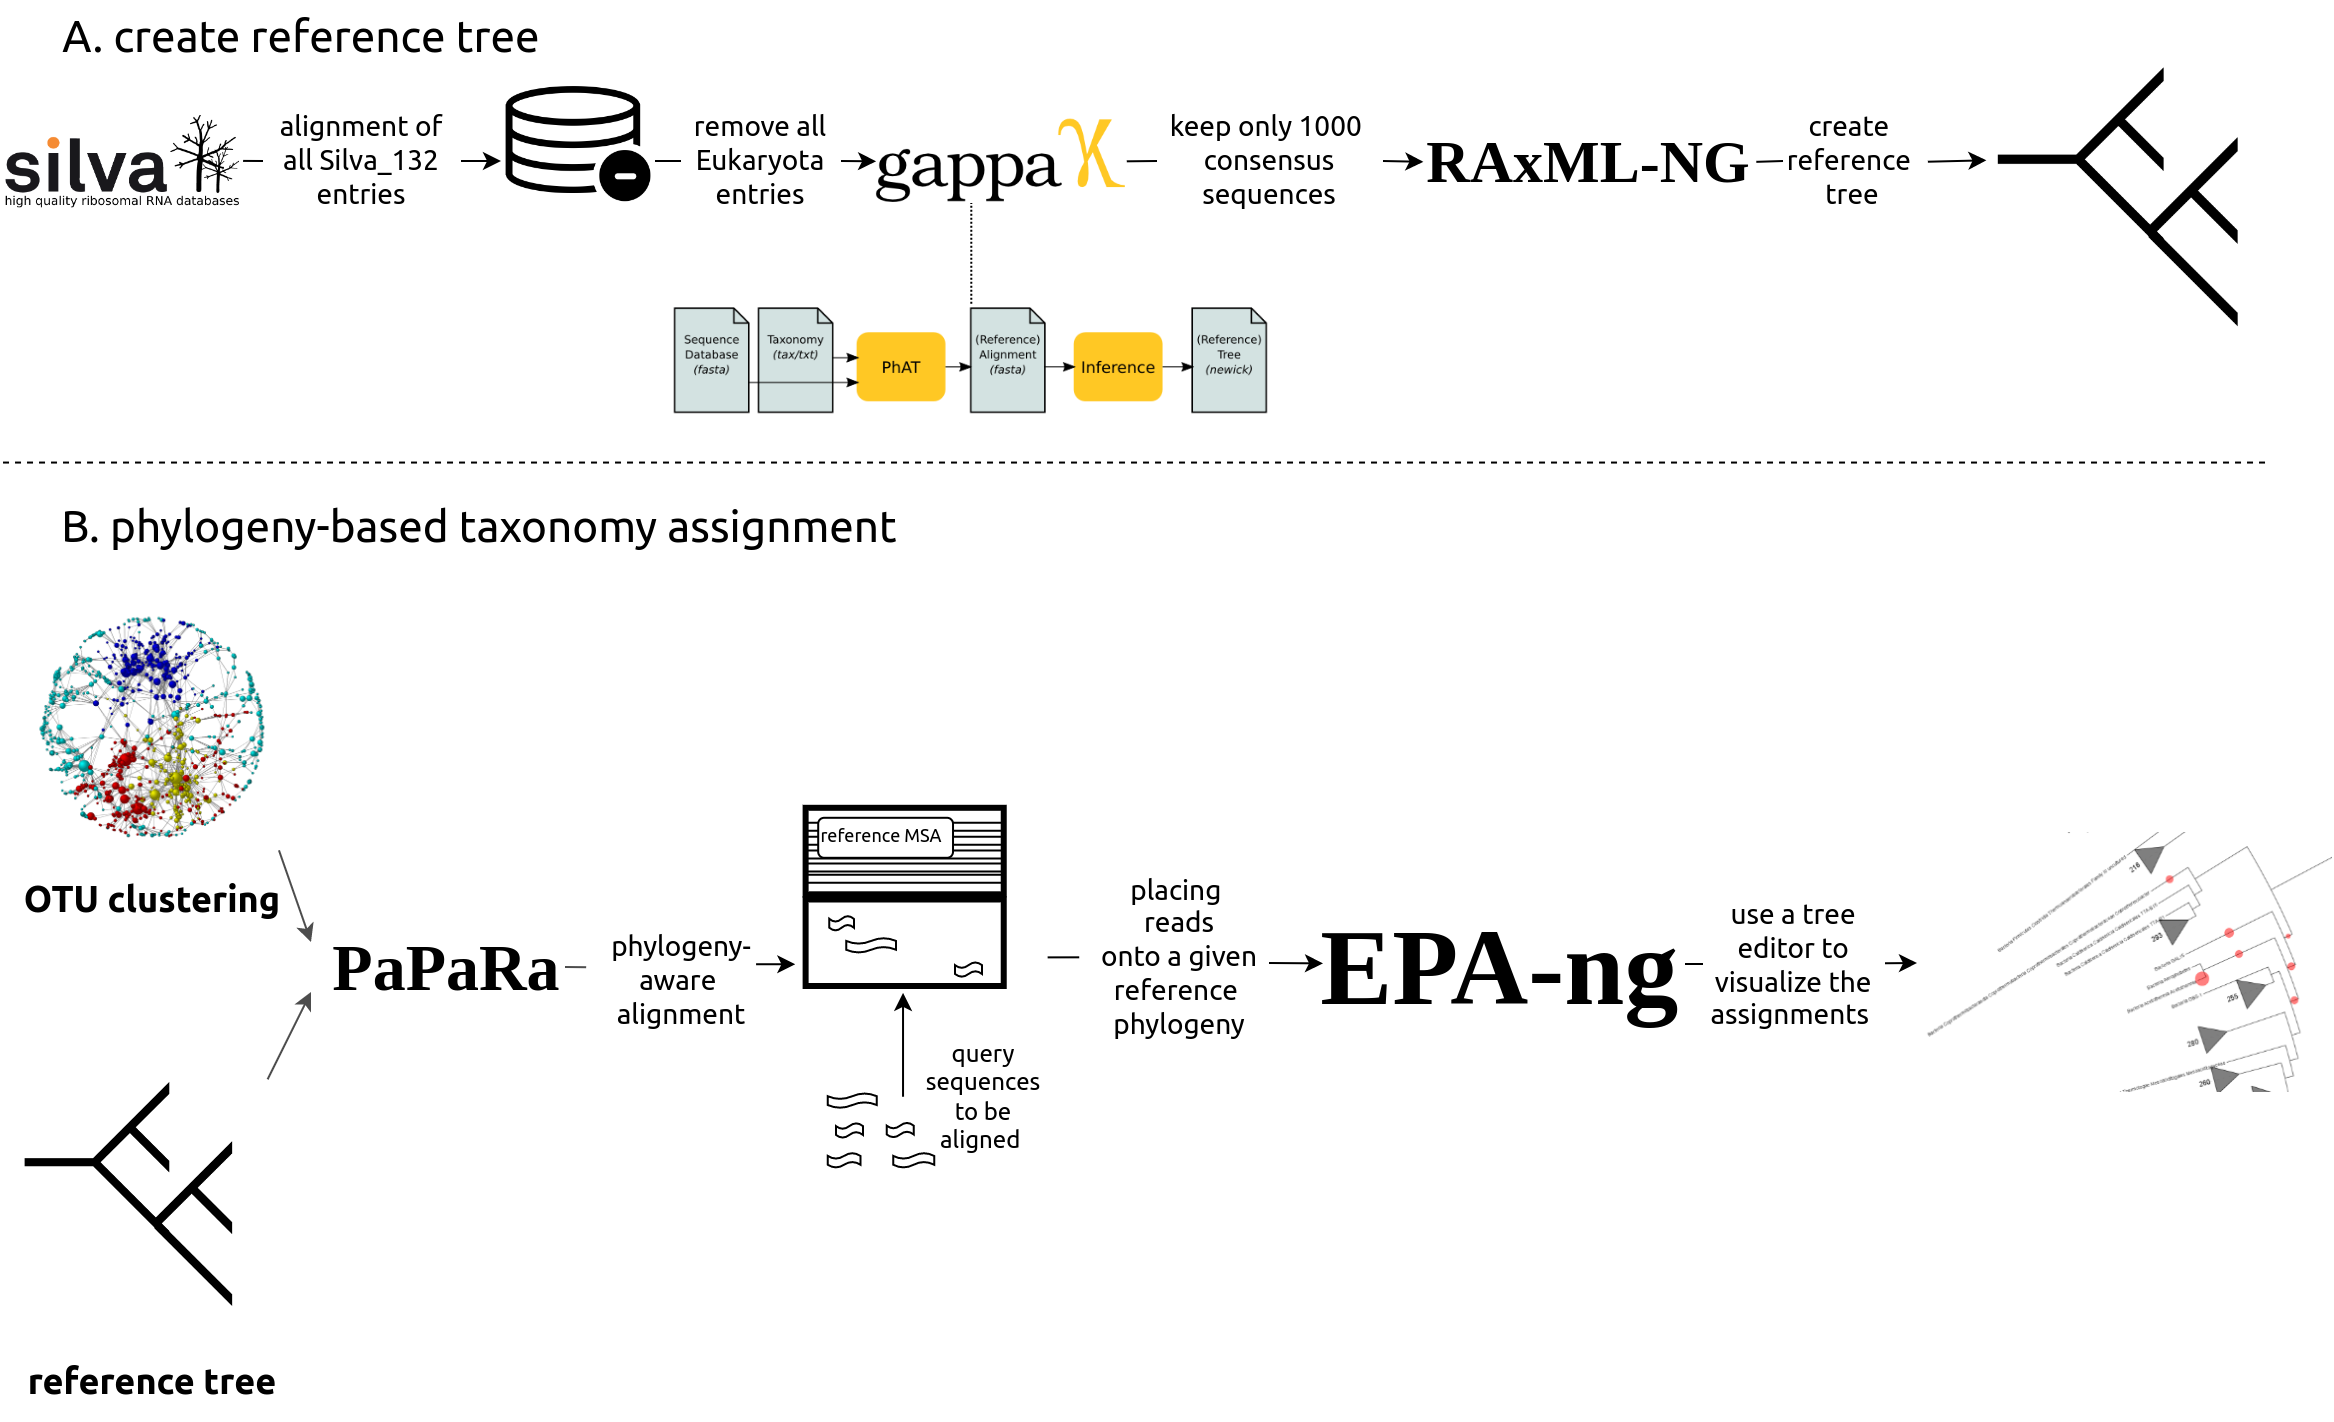
\includegraphics[width=104mm]{resources/pema_tree.png}
               };

         \end{tikzpicture}
      \end{singlespace}

      % RELATED CHAPTER
      \begin{tikzpicture}[overlay,remember picture]
         \node[anchor=west, xshift=130pt, yshift=-35pt]
         at (current page.north) {
            
\includegraphics[width=15mm]{resources/chapter2.1.png}
         };
      \end{tikzpicture}

   \end{frame}

   % MOCK COMMUNITIES 16S RESULTS
   \begin{frame}
      \frametitle{Results: tuning effetcts}
      \framesubtitle{in mock communities}

      \footnotesize Mock communities using the 16S rRNA gene and multiple parameter sets \\ 
      \footnotesize (identification at the genus level):

      % TABLE PART 1
      \begin{table}[]
         \resizebox{1.08\textwidth}{!}{%
         \hskip-2.8cm

         \begin{tabular}{l|llllllllll}
            \textbf{\begin{tabular}[c]{@{}l@{}}mock community of Gohl et al. (2016)\\ KAPA protocol\end{tabular}} & \textbf{\begin{tabular}[c]{@{}l@{}}Swarm \\ (d = 1 \\ strict = 0.8 \\ no singletons)\end{tabular}} & \textbf{\begin{tabular}[c]{@{}l@{}}Swarm \\ ( d = 1 \\ strict = 0.8 \\ with singletons)\end{tabular}} & \textbf{\begin{tabular}[c]{@{}l@{}}Swarm \\ ( d = 3 \\ strictness = 0.6 \\ no singletons)\end{tabular}} & \textbf{\begin{tabular}[c]{@{}l@{}}Swarm \\ ( d = 3 \\ strictness = 0.8\\ with singletons)\end{tabular}} & \textbf{\begin{tabular}[c]{@{}l@{}}Swarm \\ ( d = 10 \\ strictness = 0.8 \\ with singletons)\end{tabular}} & \textbf{\begin{tabular}[c]{@{}l@{}}Swarm \\ ( d = 10 \\ strictness = 0.8 \\ no singletons)\end{tabular}} & \textbf{\begin{tabular}[c]{@{}l@{}}Swarm \\ ( d = 25  \\ strictness = 0.6 )\end{tabular}} & \textbf{\begin{tabular}[c]{@{}l@{}}Swarm \\ ( d = 25 \\ strictntess = 0.8)\end{tabular}} & \textbf{\begin{tabular}[c]{@{}l@{}}Swarm \\ ( d = 30 \\ strictness = 0.6)\end{tabular}} & \textbf{\begin{tabular}[c]{@{}l@{}}Swarm \\ ( d = 30 \\ strictness = 0.8)\end{tabular}} \\ \hline
            TP & 12 &  & 15 & 18 & 18 & 15 & 17 & 17 & 17 & 17 \\
            FP & 2 &  & 2 & 21 & 11 & 6 & 5 & 5 & 4 & 5 \\
            FN & 8 &  & 5 & 2 & 2 & 5 & 3 & 3 & 3 & 3 \\
            PREC (TP / TP+FP) & 0.86 &  & 0.88 & 0.46 & 0.62 & 0.71 & 0.77 & 0.77 & 0.81 & 0.77 \\
            REC (TP / TP+FN) & 0.6 &  & 0.75 & 0.9 & 0.9 & 0.75 & 0.85 & 0.85 & 0.85 & 0.85 \\
            F1 (2 * (PREC * REC) / (PREC+REC) & 0.71 &  & \textbf{0.81} & 0.61 & 0.73 & 0.73 & 0.81 & 0.81 & 0.83 & 0.81
            \end{tabular}
         }
      \end{table}

      % TABLE PART 2
      \begin{table}
         \resizebox{0.8\textwidth}{!}{%
         \begin{tabular}{l|lll}
            \textbf{\begin{tabular}[c]{@{}l@{}}mock community of Gohl et al. (2016)\\ KAPA protocol\end{tabular}} & \textbf{\begin{tabular}[c]{@{}l@{}}vsearch\\ ( id =0.95 \\ strict = 0.8)\end{tabular}} & \textbf{\begin{tabular}[c]{@{}l@{}}vsearch\\ ( id =0.97 \\ strictness = 0.8)\end{tabular}} & \textbf{\begin{tabular}[c]{@{}l@{}}vsearch\\ ( id =0.99 \\ strictness = 0.8)\end{tabular}} \\ \hline
            TP & 11 & 12 & 12 \\
            FP & 3 & 3 & 3 \\
            FN & 9 & 8 & 8 \\
            PREC (TP / TP+FP) & 0.79 & 0.80 & 0.80 \\
            REC (TP / TP+FN) & 0.55 & 0.6 & 0.6 \\
            F1 (2 * (PREC * REC) / (PREC+REC) & 0.65 & 0.69 & 0.69
         \end{tabular}
         }
      \end{table}

      % RELATED CHAPTER
      \begin{tikzpicture}[overlay,remember picture]
         \node[anchor=west, xshift=130pt, yshift=-35pt]
         at (current page.north) {
            
\includegraphics[width=15mm]{resources/chapter2.1.png}
         };
      \end{tikzpicture}

   \end{frame}

   % REAL WORLD RESULTS
   \begin{frame}
      \frametitle{Results: Tuning effects}
      \framesubtitle{in real-world data}

      \small Using the \textit{Bista} et al. dataset (COI) and multiple \textit{d} values 
      of the Swarm algorithm

      \begin{table}[]
         \resizebox{\textwidth}{!}{%
         \begin{tabular}{llllll}
         \textbf{Parameter} & \textit{\textbf{d = 1}} & \textit{\textbf{d = 2}} & \textit{\textbf{d = 3}} & \textit{\textbf{d = 10}} & \textit{\textbf{d = 13}} \\ \hline
         \begin{tabular}[c]{@{}l@{}}MOTUs after pre-process \\ and clustering steps\end{tabular} & 83,791 & 59,833 & 33,227 & 7,384 & 4,829 \\
         MOTUs after chimera removal & 80,347 & 57,863 & 32,539 & 7,339 & 4,796 \\
         Non-singleton MOTUs & 6,381 & 4,947 & 2,658 & 1,914 & 1,634 \\
         Assigned species & 62 & 83 & 86 & 86 & 84 \\
         Execution time (h) & 2:01:35 & 2:09:49 & 1:51:44 & 2:17:26 & 2:31:15
         \end{tabular}}
      \end{table}

      % RELATED CHAPTER
      \begin{tikzpicture}[overlay,remember picture]
         \node[anchor=west, xshift=130pt, yshift=-35pt]
         at (current page.north) {
            
\includegraphics[width=15mm]{resources/chapter2.1.png}
         };
      \end{tikzpicture}

   \end{frame}

   % When PEMA was performed with the Swarm v2 algorithm (d = 3, strictness = 0.6) 
   % without removal of singletons, 18 of the 20 taxa were identified to the genus level 
   % and 3 of these even to the species level. There were 2 species that were not found 
   % in any of the PEMA runs. According to Gohl et al. [45], there was a discrepancy in the 
   % identification of those 2 species that was dependent on the amplification protocol used. 
   % It is worth mentioning that as d increases, taxa cannot be identified to species level at all; 
   % however, FP assignments decrease. Thus, when d = 30 and strictness = 0.6 for the KAPA samples, 
   % Enterococcus was not identified at all; however, PEMA finds its greatest F1 value (at the genus level, 
   % see Table 1) as the FP assignments returned are minimized. 
   % When PEMA was run using the VSEARCH clustering algorithm, high precision values were returned in all cases (>0.79). 
   % However, the recall values were decreased when using Swarm v2 (0.65–0.68).

   \if 0
   % INPUT - OUTPUT - RUN WITH A SINGLE COMMAND
   \begin{frame}
      \frametitle{Mount your I/O}
      \framesubtitle{give \& take}

      \begin{tikzpicture}[overlay,remember picture]

         \node[anchor=west, xshift=10pt, yshift=-10pt]               
            at (current page.west) {

               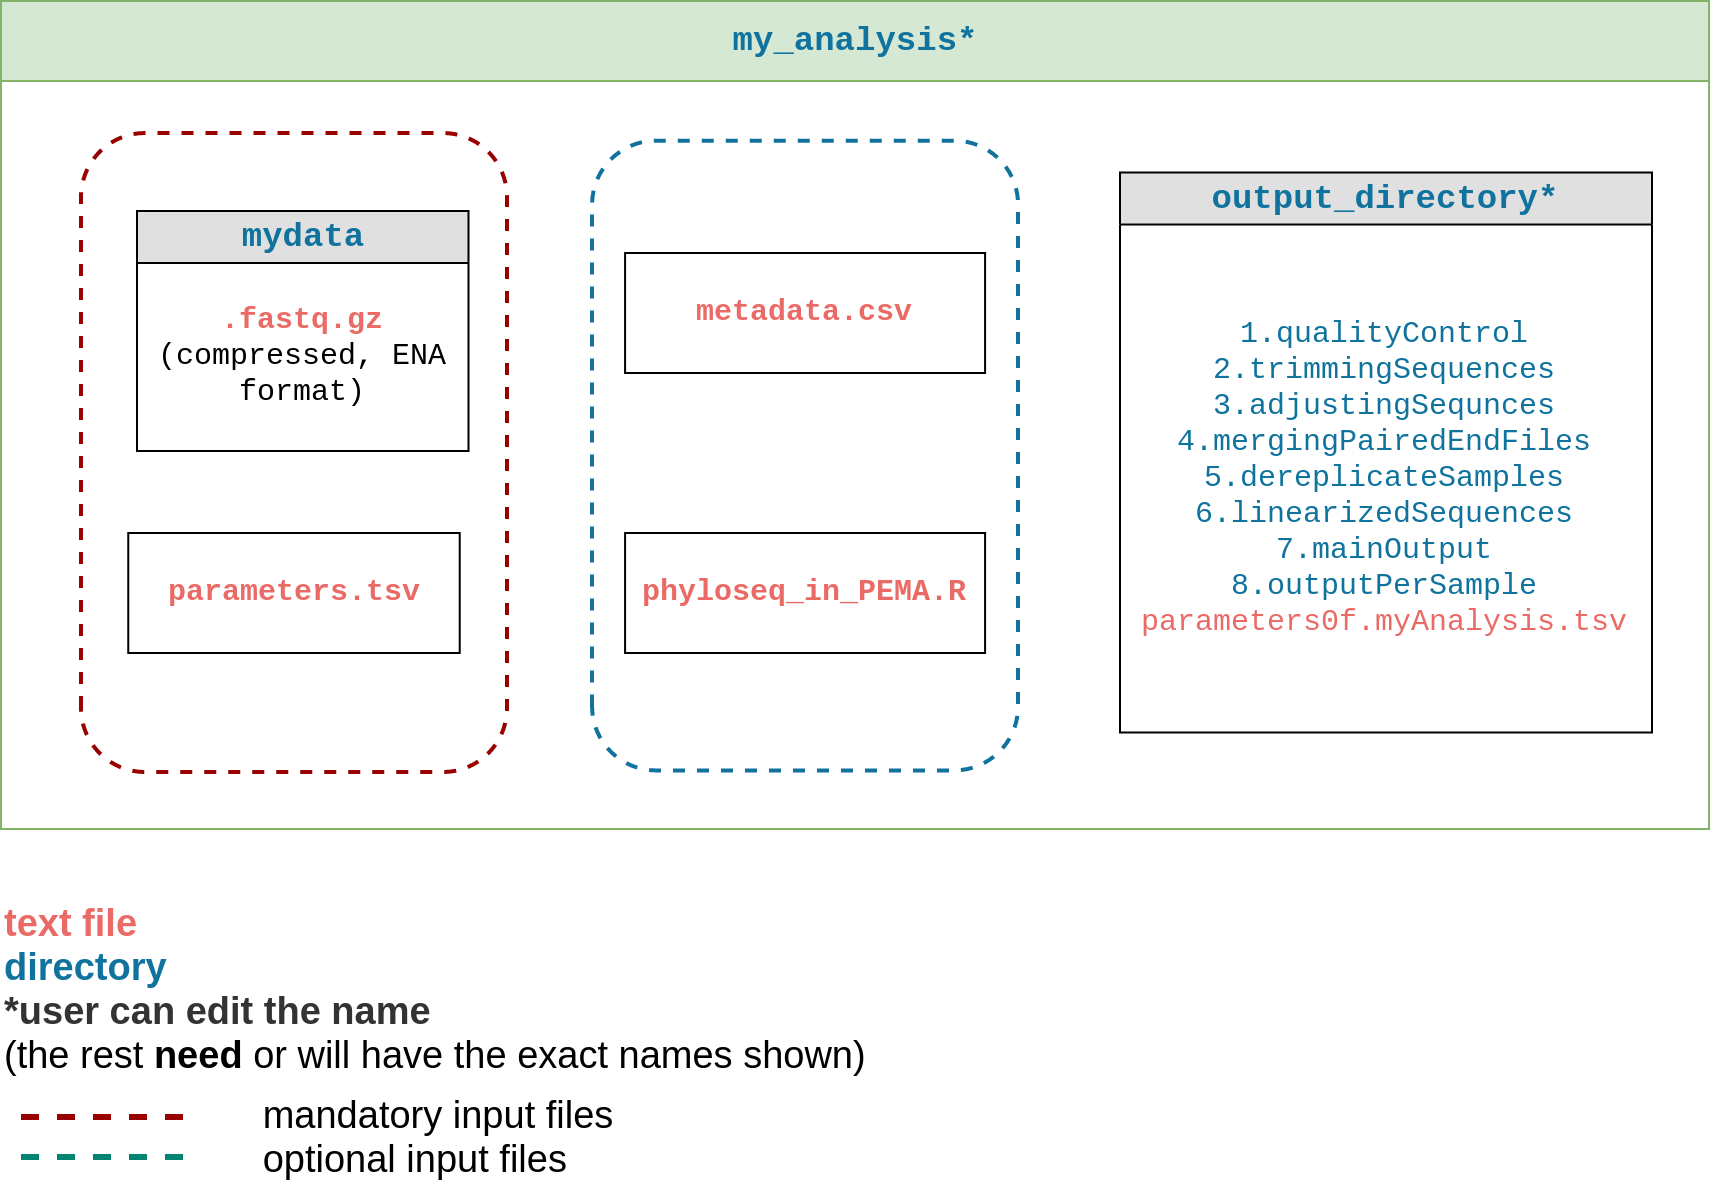
\includegraphics[width=75mm]{resources/pema_anlysis_dir-Page-1.drawio.png}
            
            };

         \node[anchor=east, xshift=-10pt, yshift=50pt]               
         at (current page.east) {

            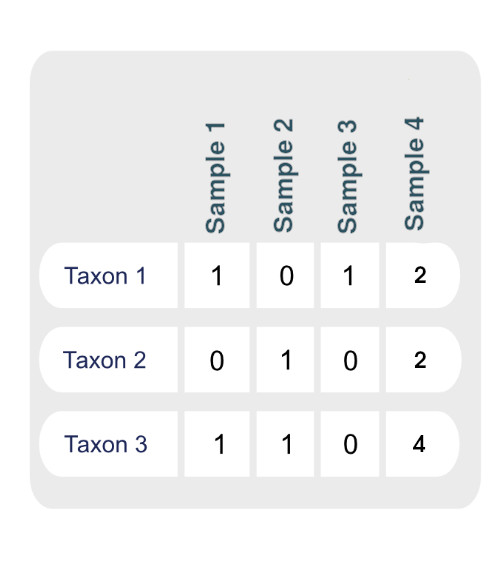
\includegraphics[width=35mm]{resources/final_table.jpg}
         
         };

         \node[anchor=east, xshift=-10pt, yshift=-60pt]
         at (current page.east) {

            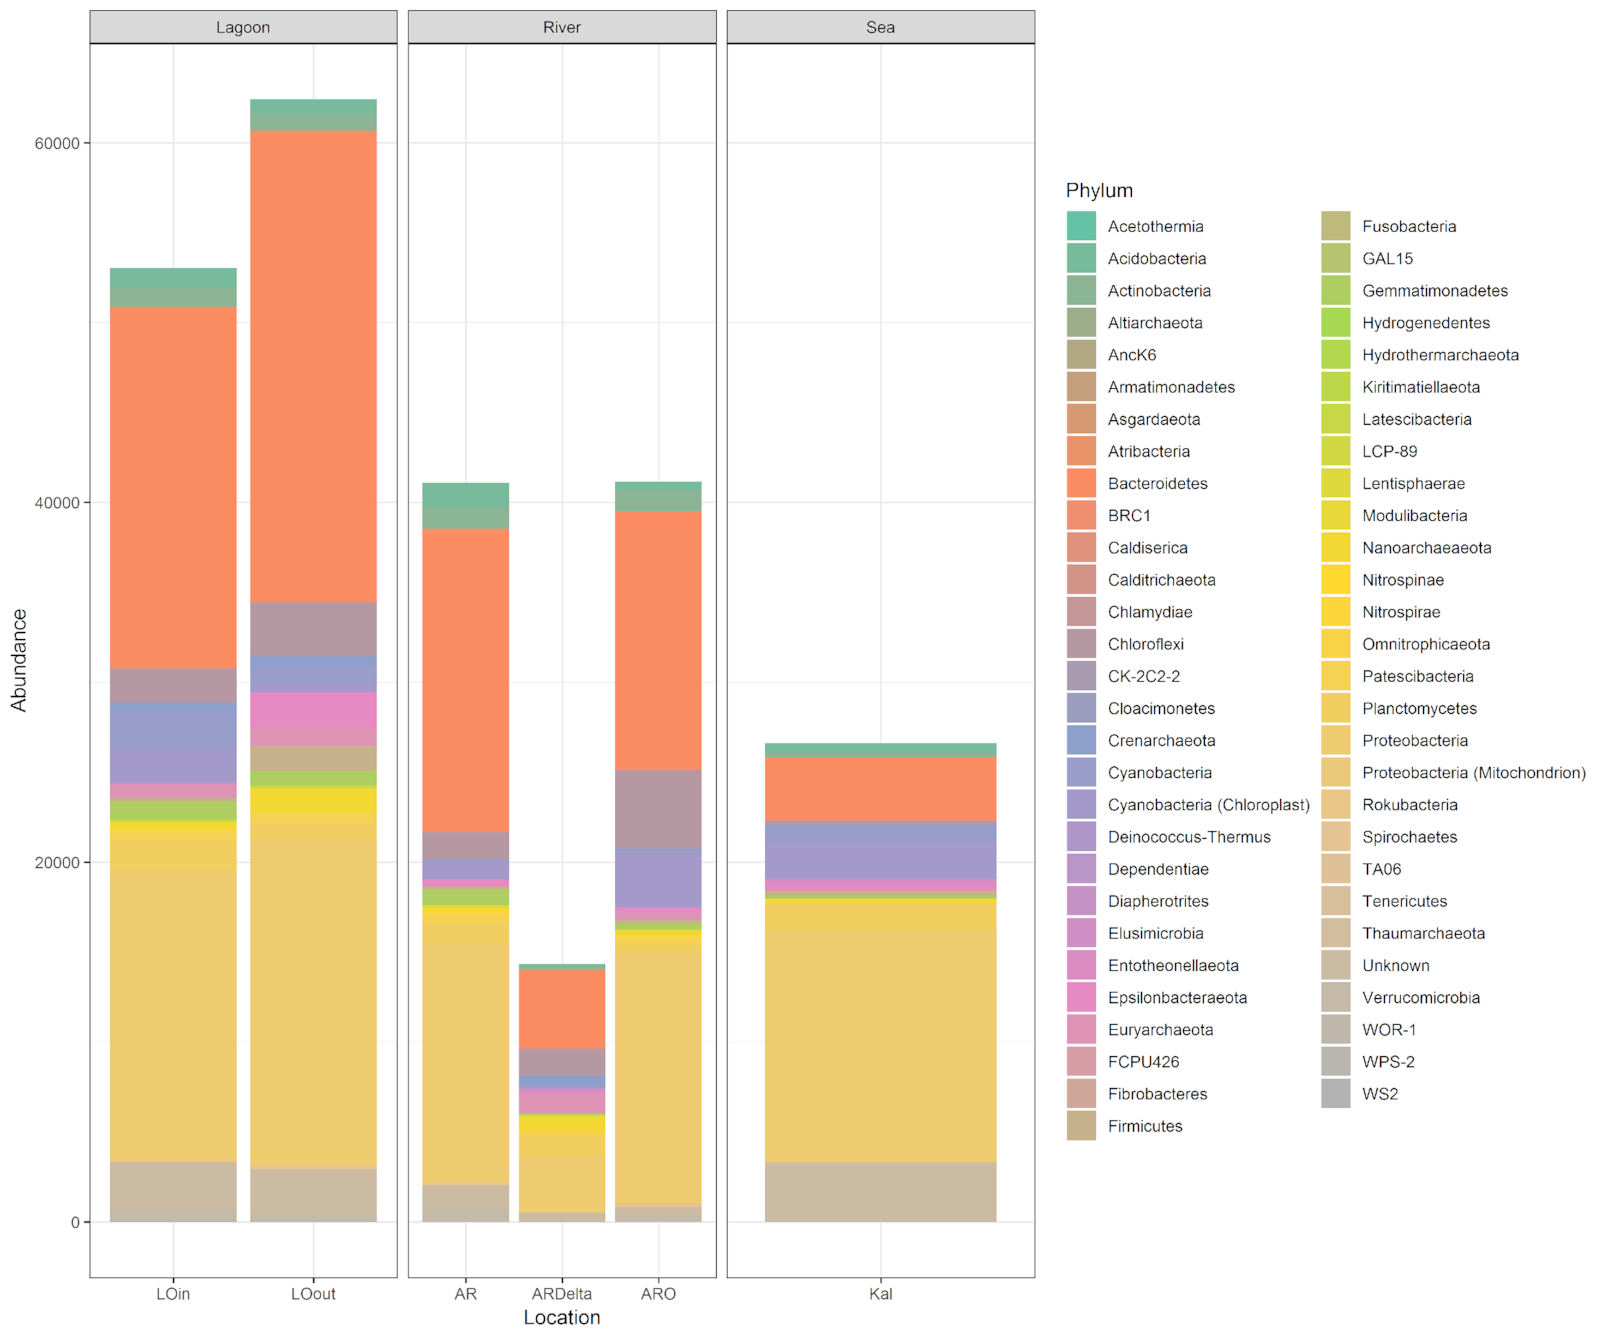
\includegraphics[width=43mm]{resources/giaa022fig3.jpeg}
         
         };


      \end{tikzpicture}
      
   
   \end{frame}
   \fi

   % PEMA PUBLICATION 
   \if 0 
   \begin{frame}
      \frametitle{PEMA publication}
      \framesubtitle{in 2020}
      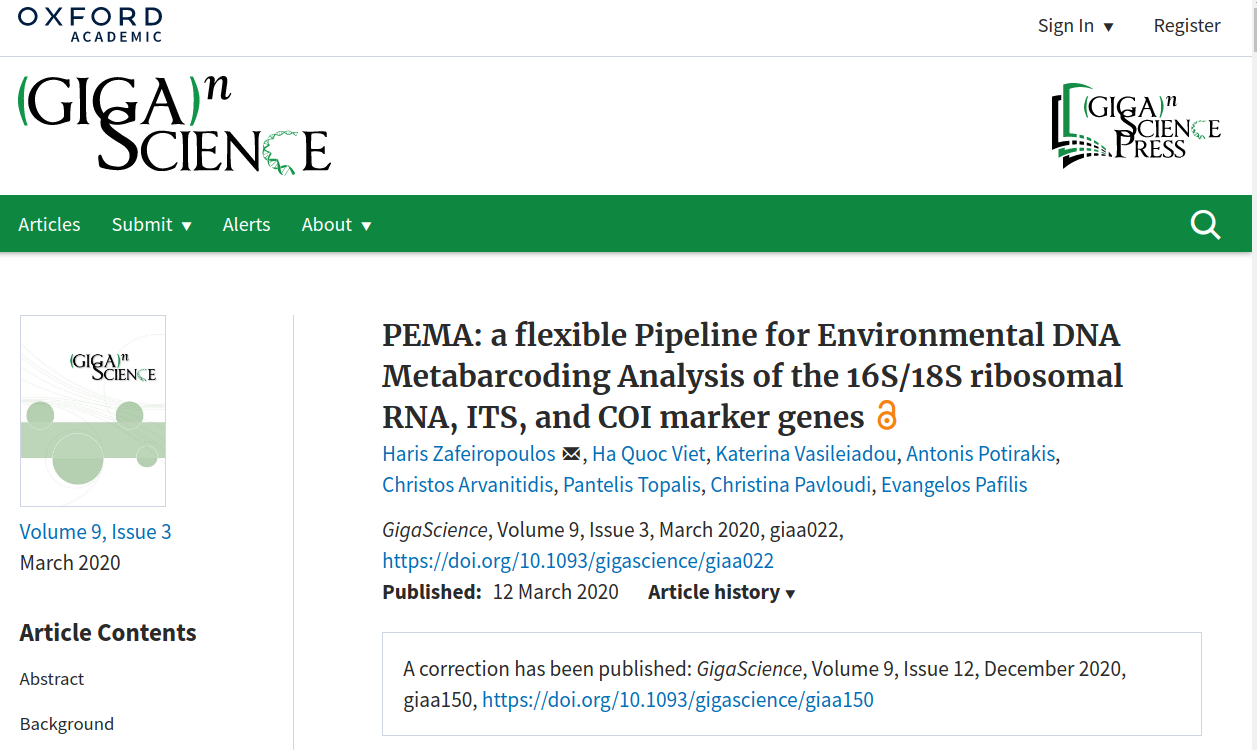
\includegraphics[width=100mm]{resources/pema_publ.png}
   \end{frame}
   \fi 

   % PEMA VERSION 2
   \begin{frame}
      \frametitle{PEMA v.2}
      \framesubtitle{addressing some of the challenges}

      \begin{singlespace}
         \begin{tikzpicture}[overlay,remember picture]
       
               \node[anchor=west, xshift=30pt,yshift=-150pt]
                  at (current page.north west) {
                     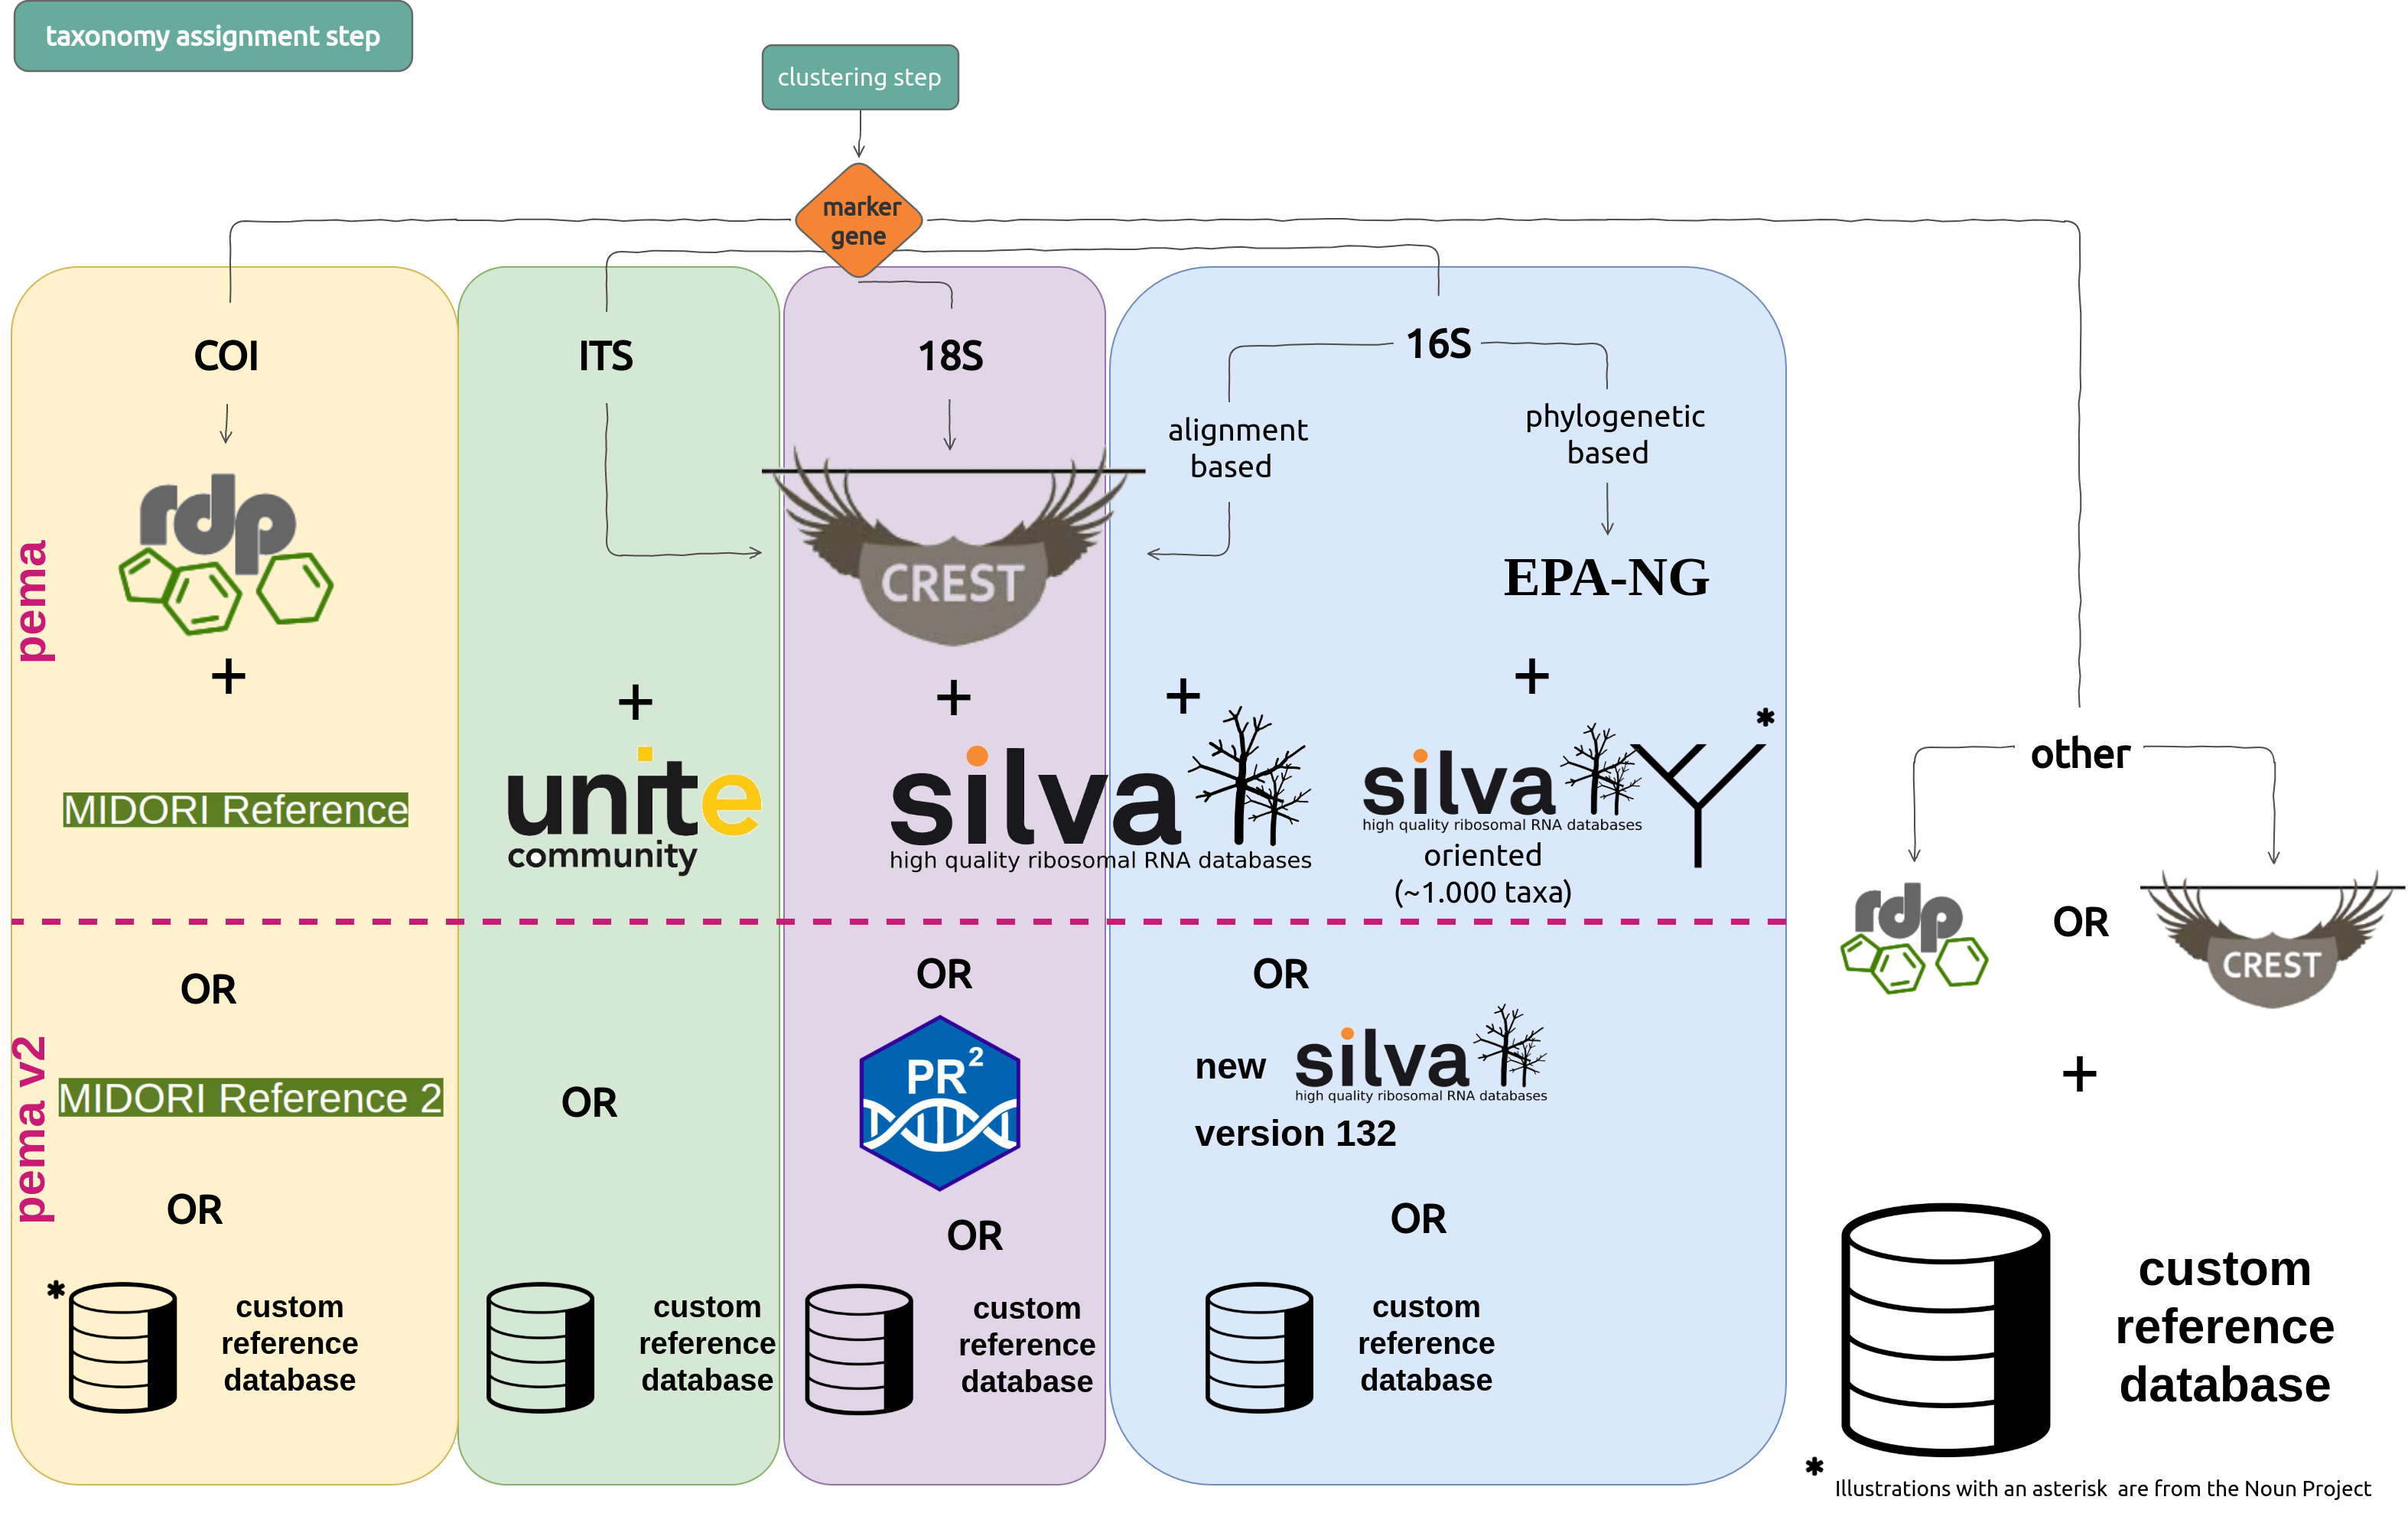
\includegraphics[width=100mm]{resources/pema-pema.v2.drawio.png}
                  };
                  
         \end{tikzpicture}

         \begin{textblock*}{5cm}(8.2cm, 2.3cm) % {block width} (coords) 
            
            \scriptsize Code architecture from scratch!

         \end{textblock*}

      \end{singlespace}
      % RELATED CHAPTER
      \begin{tikzpicture}[overlay,remember picture]
         \node[anchor=west, xshift=130pt, yshift=-35pt]
         at (current page.north) {
            
\includegraphics[width=15mm]{resources/chapter2.1.png}
         };
      \end{tikzpicture}

   \end{frame}

   % PEMA v.2.1.4 - ARMS
   \begin{frame}
      \frametitle{Latest PEMA version}
      \framesubtitle{addressing the challenges of the community}

      \begin{singlespace}
         \begin{tikzpicture}[overlay,remember picture]
       
               \node[anchor=west, xshift=30pt,yshift=-150pt]
                  at (current page.north west) {
                     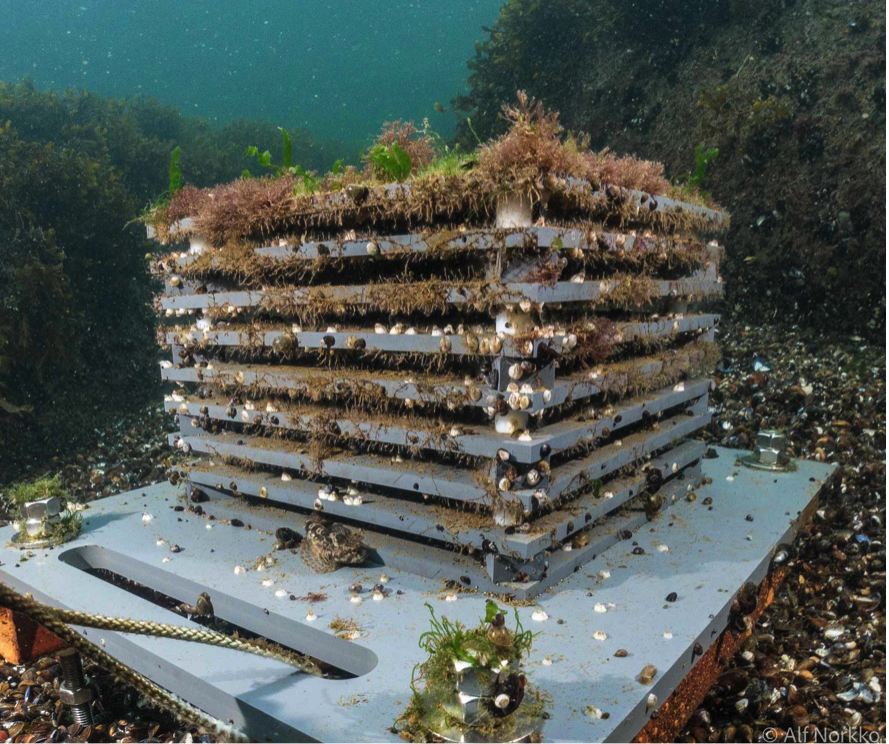
\includegraphics[width=55mm]{resources/Autonomous-Reef-Monitoring.png}
               };

               \node[anchor=east, xshift=-65pt,yshift=50pt]
                  at (current page.east) {
                     
\includegraphics[width=34mm]{resources/assemble_logo.png}
               };

               \node[anchor=east, xshift=-5pt,yshift=50pt]
                  at (current page.east) {
                     
\includegraphics[width=17mm]{resources/MBON_logo_transparent.png}

               };

         \end{tikzpicture}


         \begin{textblock*}{5cm}(7.2cm,4.0cm) % {block width} (coords) 
            
            \scriptsize

            \textbf{\texttt{pema:v.2.1.4} includes:}

            \begin{enumerate}
               \item analysis of 12S rRNA data now supported
                     (\href{https://github.com/terrimporter/12SvertebrateClassifier/releases}{12S Vertebrate Classifier v2.0.0-ref} database) 
               \item PR2 as an alternative reference 
                     database for the case of 18S rRNA 
               \item the \texttt{ncbi-taxonomist} tool \\ 
                     was added to return the NCBI Taxonomy \\ 
                     Id of the taxonomies found
            \end{enumerate}
         \end{textblock*}
      \end{singlespace}

      % RELATED CHAPTER
      \begin{tikzpicture}[overlay,remember picture]
         \node[anchor=west, xshift=130pt, yshift=-35pt]
         at (current page.north) {
            
\includegraphics[width=15mm]{resources/chapter2.1.png}
         };
      \end{tikzpicture}

   \end{frame}

   % PEMA WEBSITE
   \if 0
   \begin{frame}
      \frametitle{\textit{How to} and further documentation}
      \framesubtitle{at \href{http://pema.hcmr.gr}{pema.hcmr.gr}}
      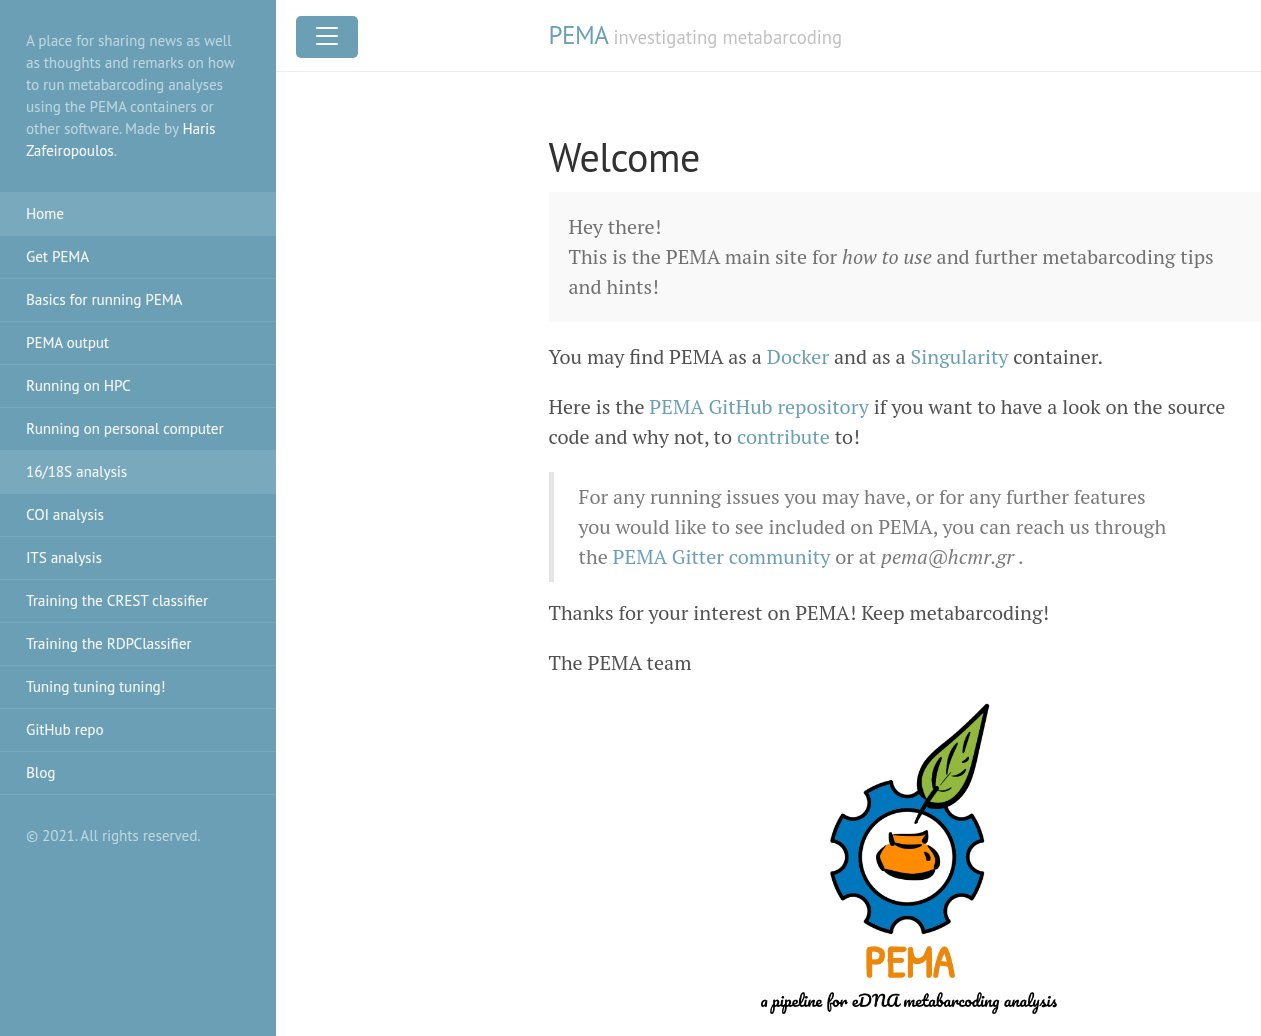
\includegraphics[width=85mm]{resources/pema_site.png}
      % add citation and logo
   \end{frame}
   \fi 

   % % PEMA @ LW ERIC
   \begin{frame}
      \frametitle{Moving at the large scale}
      \framesubtitle{PEMA @ infrustuctures}
      \begin{singlespace}
         \begin{tikzpicture}[overlay,remember picture]
       
               \node[anchor=west, xshift=30pt,yshift=-150pt]
                  at (current page.north west) {
                     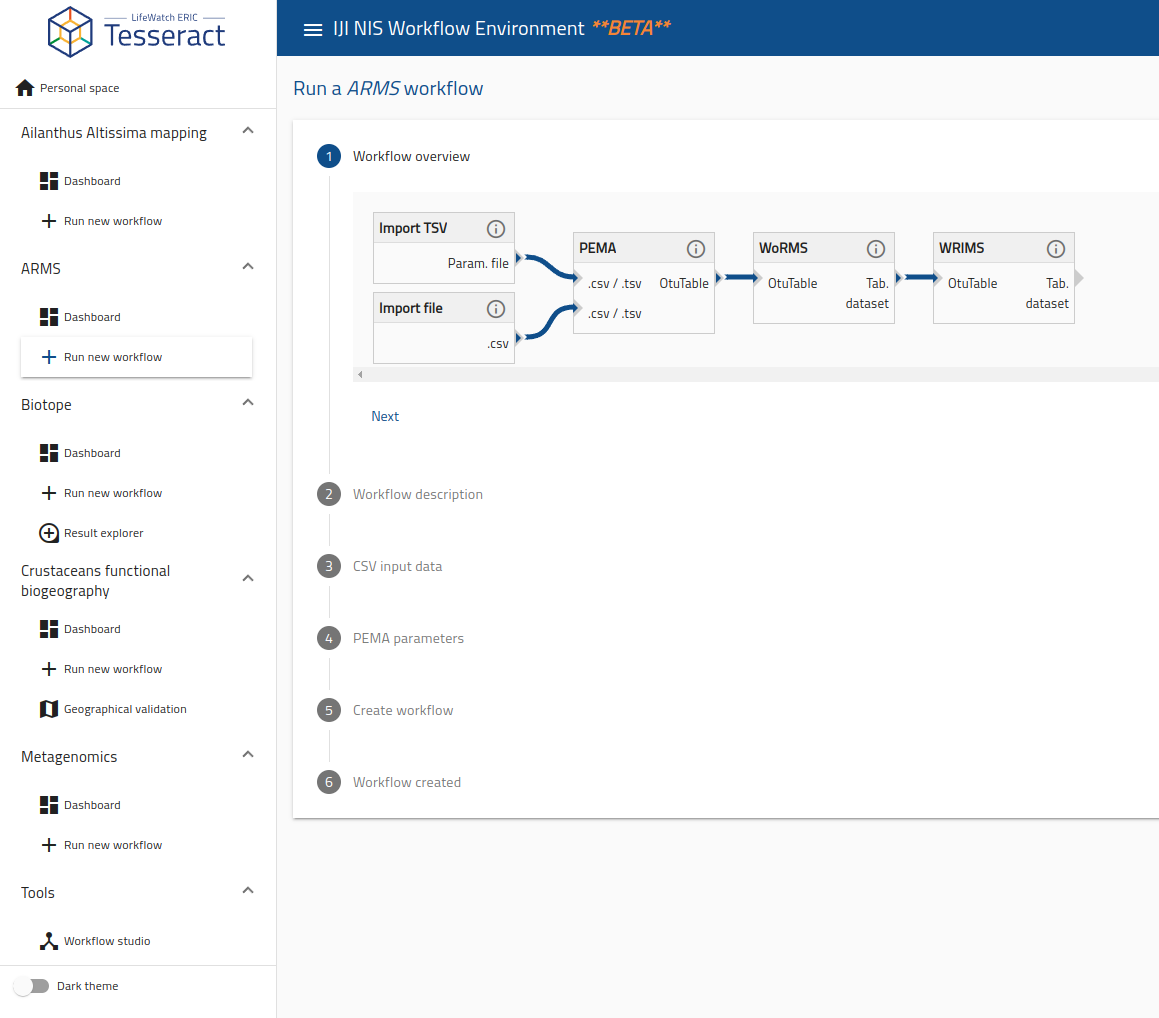
\includegraphics[width=55mm]{resources/pema_lw.png}
               };

         \end{tikzpicture}

         \begin{textblock*}{5cm}(7.2cm,4.0cm) % {block width} (coords) 
            

            \begin{enumerate}
               \item \small Web - interface make analysis even easier
               \item \small researchers without access to HPC/clouds etc are now able to run big scale analyses
               \item \small Combine with other tools
            \end{enumerate}

         \end{textblock*}
         \end{singlespace}
      % RELATED CHAPTER
      \begin{tikzpicture}[overlay,remember picture]
         \node[anchor=west, xshift=130pt, yshift=-35pt]
         at (current page.north) {
            
\includegraphics[width=15mm]{resources/chapter2.1.png}
         };
      \end{tikzpicture}

   \end{frame}

   % EOSC Life GOs
   \if 0
   \begin{frame}
      \frametitle{Metagenome go deeper than amplicon studies}
      \framesubtitle{yet come with vast computational challenges}
      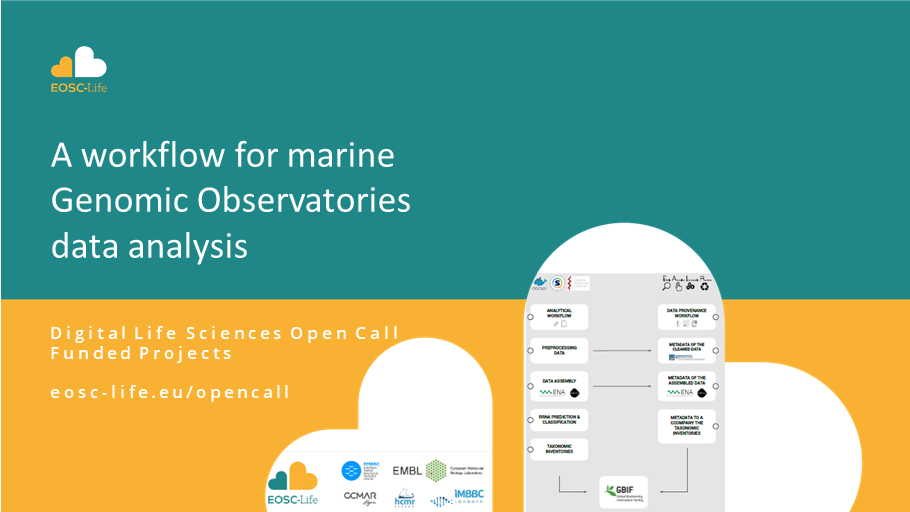
\includegraphics[width=70mm]{resources/marine-genomic-observatories.png}

      \begin{textblock*}{5cm}(8.5cm,4.0cm) % {block width} (coords) 
            
         \textbf{Work in progress} \\
         To be available in the \\ months to come.

         \bigskip
         
         \footnotesize
         You may find more \\ 
         \footnotesize
         about this project  \\
         \footnotesize
         through its \href{https://github.com/emo-bon/pipeline-v5}{GitHub repository}

      \end{textblock*}
   \end{frame}
   \fi

   % PEMA CONCLUSIONS
   \begin{frame}
      \frametitle{Conclusions}
      \framesubtitle{on PEMA and eDNA metabarcoding}

      \begin{itemize}
         \item PEMA is accurate, execution-friendly and fast pipeline 
         \item tuning is essential in metabarcoding analyses
         \item sequencing a mock community along with your samples can be of great help in parameter tuning 
         \item computing resources required range; infrustuctures may benefit studies with great number of samples and CLI non-familiar users
      \end{itemize}

      % RELATED CHAPTER
      \begin{tikzpicture}[overlay,remember picture]
         \node[anchor=west, xshift=130pt, yshift=-35pt]
         at (current page.north) {
            
\includegraphics[width=15mm]{resources/chapter2.1.png}
         };
      \end{tikzpicture}

   \end{frame}


   % -------------------------------------
   % CHANGE SUBSECTION: DARN
   % -------------------------------------

   % PEMA SUBSECTION
   \begin{darkframes}
      \subsection{DARN: investigating the known unknowns in COI amplicon data}
   \end{darkframes}
   
    % AIM OF STUDY
   \begin{darkframes}
      \begin{frame}
         \frametitle{The Dark mAtteR iNvestigator (DARN) tool: getting to know
         the known unknowns in COI amplicon data}
         \framesubtitle{Aim of the study and contribution}

         To build a framework for extracting non-target, potentially unassigned 
         (or assigned with low confidence) sequences from COI environmental
         sequence samples ("dark matter") \\
         \bigskip
         We argue that the vast majority of these sequences represent
         microbial taxa, such as bacteria and archaea

      \end{frame}
   \end{darkframes}

   % DARN METHODOLOGY
   \begin{frame}
      \frametitle{Methodology / Implementation}
      \framesubtitle{Dark mAtteR iNvesigator}

      \begin{textblock*}{7cm}(1.2cm, 3.5cm)
         \small In COI amplicon studies, \\
         \small a great number of OTUs/ASVs retrieved \\
         \small either have no hits or \\
         \small their hit has a low confidence \\
         \bigskip
         \small DARN estimates to what extent \\
         \small the OTUs/ASVs retrieved in an \\ 
         \small environmental sample represent \\ 
         \small target taxa or not 
      \end{textblock*}

      \begin{singlespace}
         \begin{tikzpicture}[overlay,remember picture]
            \node[anchor=north east,yshift=-5pt]
               at (current page.north east) {
                  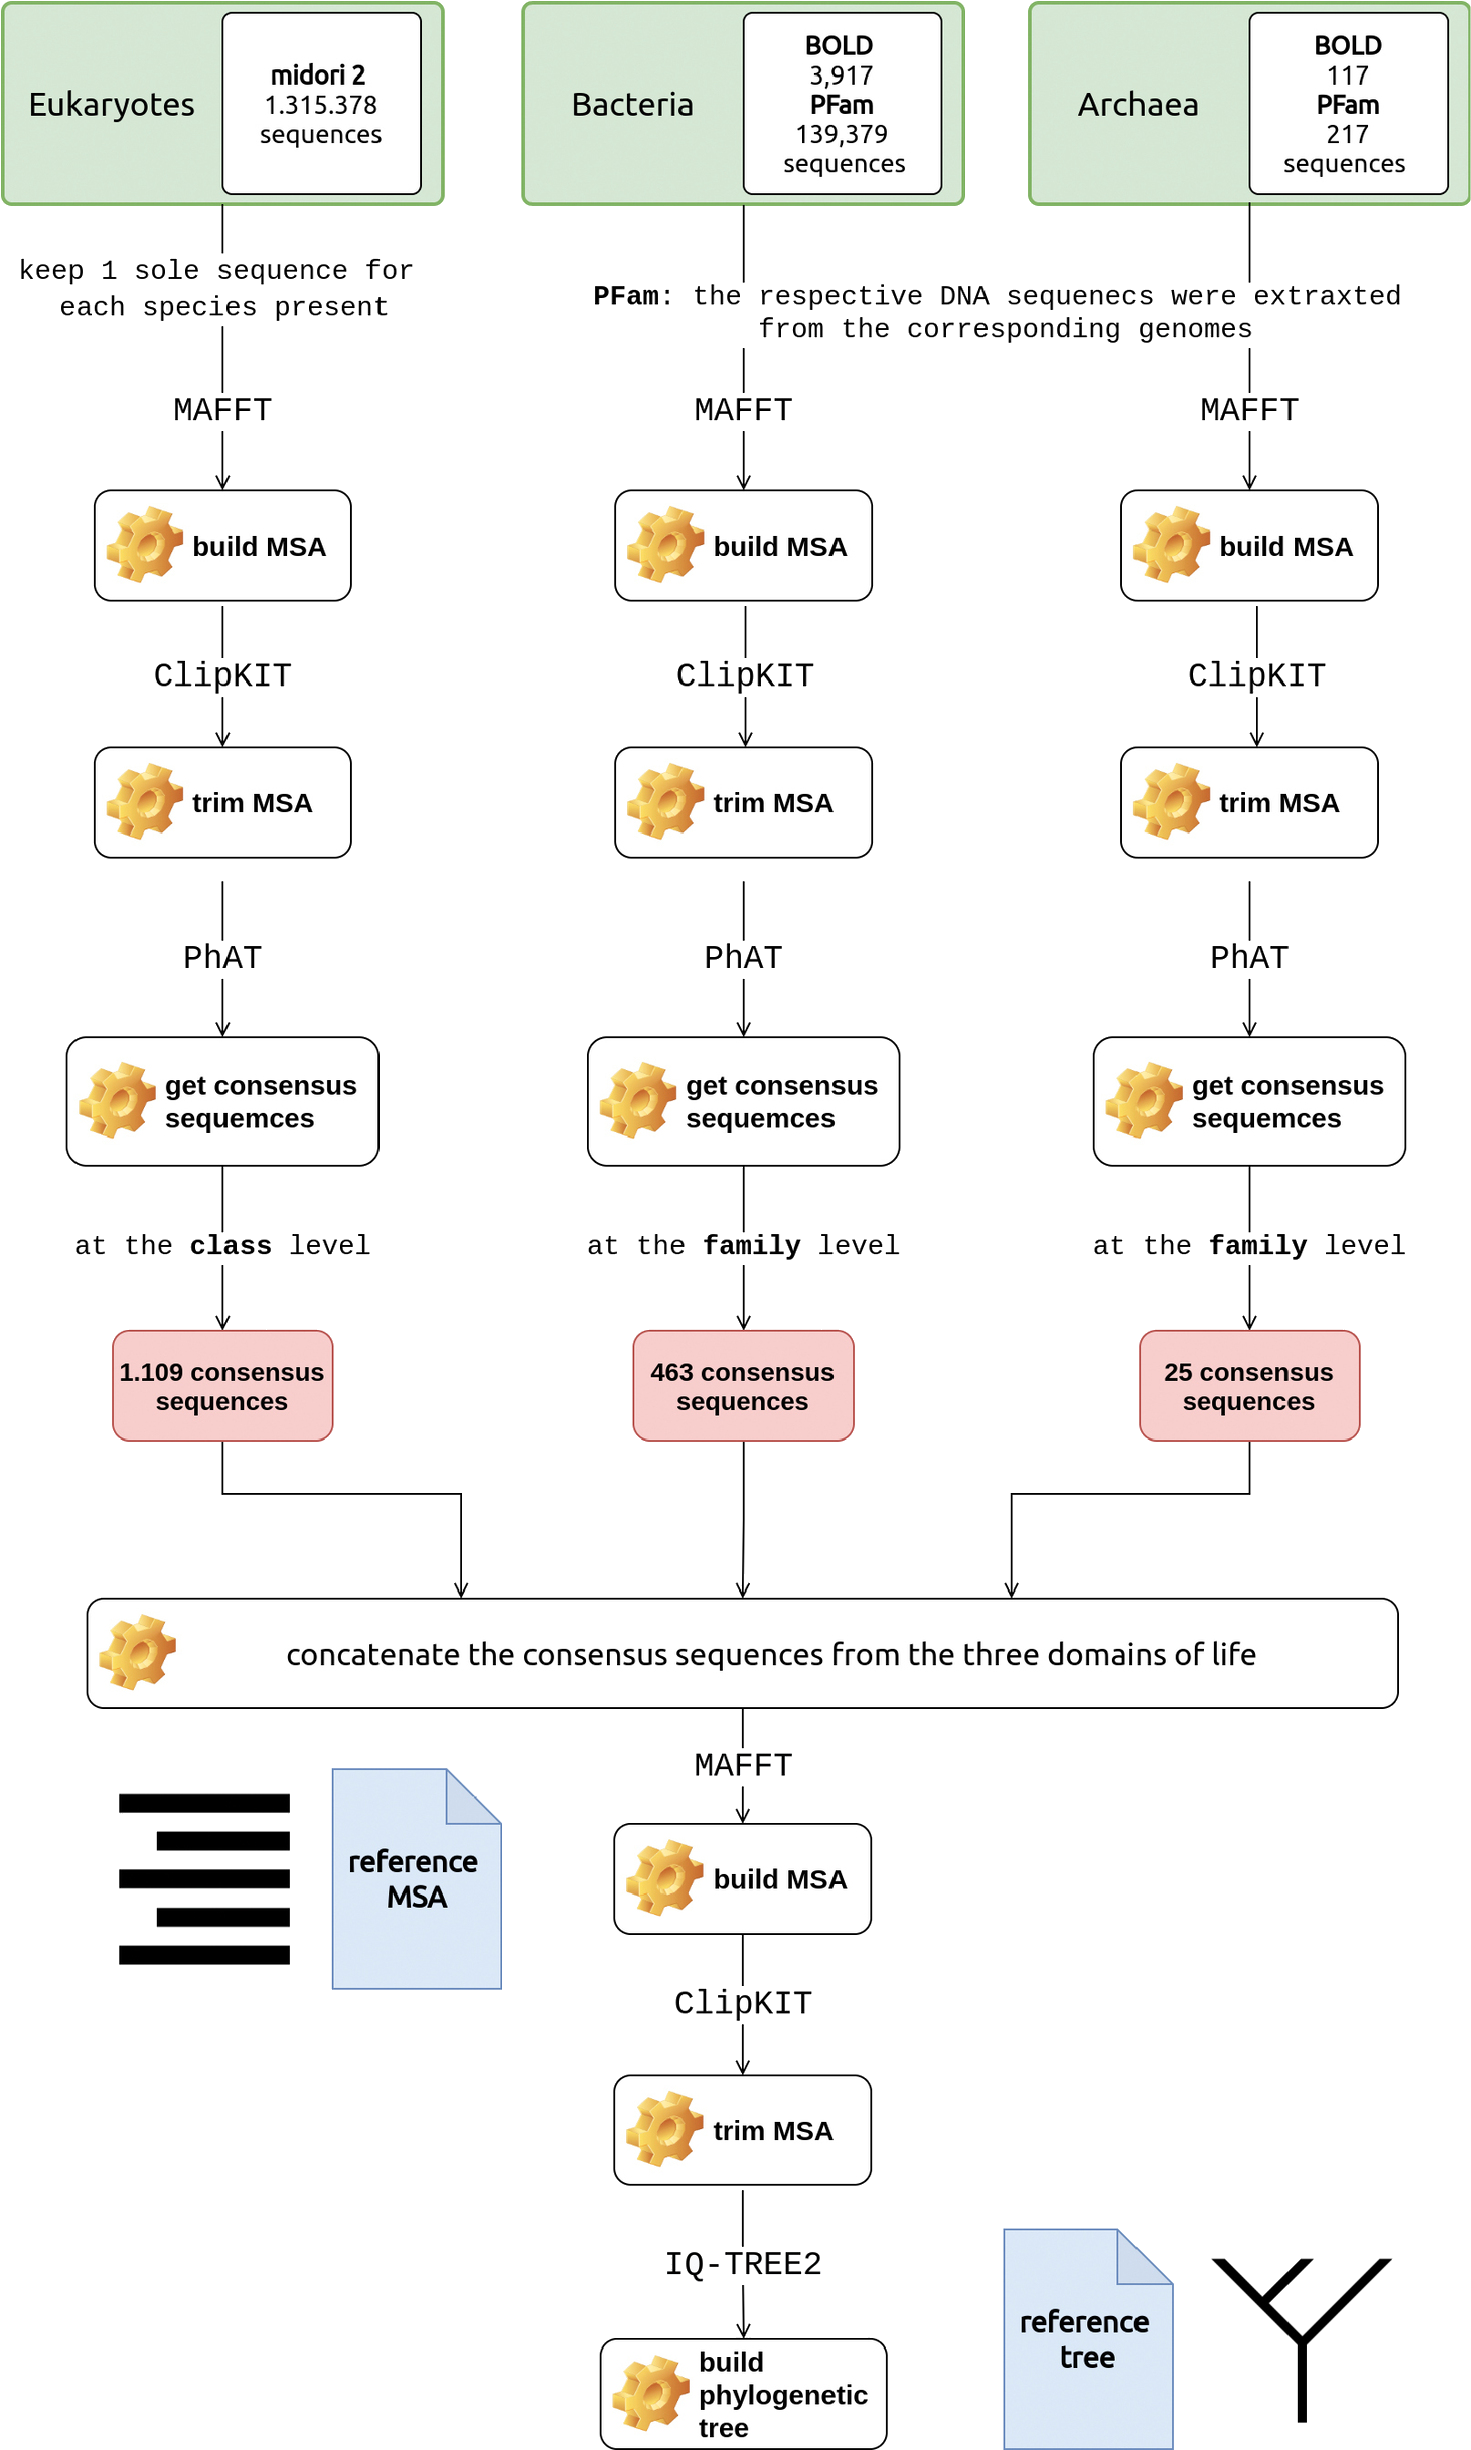
\includegraphics[width=50mm]{resources/darn_methodology_transparent.png}
               };
            \node[align = right, above, xshift=110, yshift=10] at (current page.south) {
               \tiny 
               Figure from: \href{https://doi.org/10.3897/mbmg.5.69657}{10.3897/mbmg.5.69657}
            };
         \end{tikzpicture}
      \end{singlespace}
      % RELATED CHAPTER
      \begin{tikzpicture}[overlay,remember picture]
         \node[anchor=east, xshift=-110pt, yshift=25pt]
         at (current page.south) {
            
\includegraphics[width=15mm]{resources/chapter2.2.png}
         };
      \end{tikzpicture}
   \end{frame}

   % SEQUENCES RETRIEVED
   \begin{frame}
      \frametitle{Methodology / Implementation}
      \framesubtitle{sequences retrieved}

      \begin{table}[]
         \resizebox{\textwidth}{!}{%
         \begin{tabular}{lllll}
         \hline
         \multirow{2}{*}{\textbf{Resources}} & \multicolumn{2}{l}{\textbf{bacteria}} & \multicolumn{2}{l}{\textbf{archaea}} \\ \cline{2-5} 
         & \textbf{\# of sequences} & \textbf{\# of strains} & \textbf{\# of sequences} & \textbf{\# of strains} \\ \hline
         BOLD & 3,917 & 2,267 & 117 & 117 \\
         PFam-oriented & 9,154 & 4,532 & 217 & 115 \\ \hline
         \textbf{Total unique entries} & \textbf{11,421} & \textbf{6,798} & \textbf{334} & \textbf{201}
         \end{tabular}}
      \end{table}
      % RELATED CHAPTER
      \begin{tikzpicture}[overlay,remember picture]
         \node[anchor=west, xshift=130pt, yshift=-35pt]
         at (current page.north) {
            
\includegraphics[width=15mm]{resources/chapter2.2.png}
         };
      \end{tikzpicture}
   \end{frame}

   % DARN PHYLOGENY TREE
   \begin{frame}
      \frametitle{Methodology / Implementation}
      \framesubtitle{Phylogenetic tree of the COI consensus sequences retrieved}
      \begin{tikzpicture}[overlay, remember picture]
         \node[anchor=west, xshift=10pt, yshift=-15pt]
         at (current page.west){
            \includegraphics[width=60mm]{resources/placements_of_consensus_seqs_transpaernt.png}
         };
      \end{tikzpicture}

      \begin{textblock*}{7cm}(7.0cm, 4.5cm)
         
         the consensus sequences have  \\ 
         been placed in their corresponding \\ 
         taxonomic branches, proving \\
         the tree valid

      \end{textblock*}
      % RELATED CHAPTER
      \begin{tikzpicture}[overlay,remember picture]
         \node[anchor=west, xshift=130pt, yshift=-35pt]
         at (current page.north) {
            
\includegraphics[width=15mm]{resources/chapter2.2.png}
         };
      \end{tikzpicture}
   \end{frame}

   % DARN OUTPUT
   \begin{frame}
      \frametitle{Results: DARN using real-world data}
      \framesubtitle{with multiple sample types, primers, PCR protocols and bioinormatics pipelines}

      \begin{tikzpicture}[overlay, remember picture]
         \node[anchor=west, xshift=-20pt, yshift=-20pt]
         at (current page.west){
            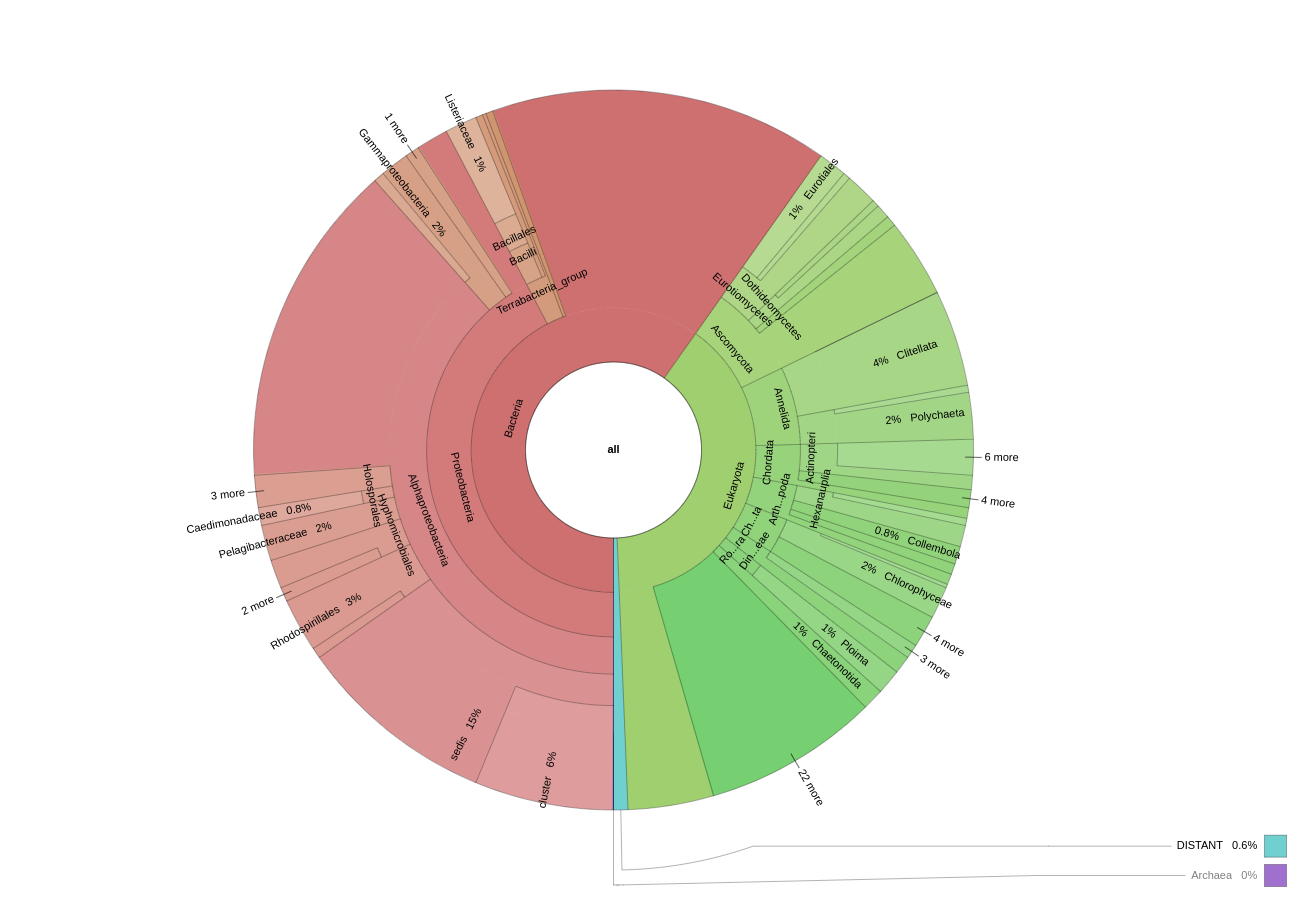
\includegraphics[width=90mm]{resources/darn_krona_output.png}
         };
      \end{tikzpicture}

      \begin{textblock*}{6cm}(7cm, 3.5cm)
         bacterial sequences are \\ 
         omnipresent in COI amplicon data \\
         \bigskip
         More results at:
         \href{https://hariszaf.github.io/darn/}{https://hariszaf.github.io/darn/} \\
      \end{textblock*}
      % RELATED CHAPTER
      \begin{tikzpicture}[overlay,remember picture]
         \node[anchor=west, xshift=130pt, yshift=-35pt]
         at (current page.north) {
            \includegraphics[width=15mm]{resources/chapter2.2.png}
         };
      \end{tikzpicture}
   \end{frame}

   % DARN CONCLUSIONS
   \begin{frame}
      \frametitle{Conclusions}
      \framesubtitle{on DARN and COI amplicon studies}
      \begin{itemize}
         \item \small bacteria, algae, fungi etc. was verified to be present in COI amplicon data
         \item \small bacteria make up a significant proportion of sequences generated in COI based eDNA metabarcoding datasets
         \item \small dark matter seems to be particularly common in eDNA as compared to bulk samples
         \item \small DARN supports quality control and further investigation of the unassigned OTUs/ASVs and
               \small allows researchers to better understand the known unknowns
      \end{itemize}
      % RELATED CHAPTER
      \begin{tikzpicture}[overlay,remember picture]
         \node[anchor=west, xshift=130pt, yshift=-35pt]
         at (current page.north) {
            \includegraphics[width=15mm]{resources/chapter2.2.png}
         };
      \end{tikzpicture}

   \end{frame}


   % -------------------------------------
   % CHANGE THE CHAPTER SLIDE: PREGO
   % -------------------------------------

   \begin{darkframes}
      \section{
         % \textbf{Chapter 3:} 
         PREGO: linking processes environments and organisms
      }
   \end{darkframes}

   % PREGO LOGO - SLIDE
   \if 0
   \begin{frame}
      
      \begin{figure}
         \includegraphics[width=75mm]{resources/prego_logo.png}
      \end{figure}

      \begin{textblock*}{12cm}(0cm, 7cm)
         \centering
         \small related repositories under \\
         \small \href{https://github.com/orgs/lab42open-team}{https://github.com/orgs/lab42open-team} \\ 
         \small web-app under\\
         \small \href{http://prego.hcmr.gr/}{http://prego.hcmr.gr/}
      \end{textblock*}

   \end{frame}
   \fi

    % AIM OF STUDY
    \begin{darkframes}
      \begin{frame}
         \frametitle{\textbf{Chapter 3}: PREGO: a literature- and data-mining
         resource to associate microorganisms,
         biological processes, and
         environment types}
         \framesubtitle{Aim of the study and contribution}

         \small
            To build a hypothesis generation resource based on associations between: 
            \begin{itemize}
               \item \textit{organisms} and the \textit{environments} they inhabit
               \item \textit{organisms} and the biological \textit{processes} they are involved with
               \item \textit{processes} and the \textit{environments} where they occur
            \end{itemize}

            To this end, associations among such terms were exported from: 
            \begin{itemize}
               \item the publicaly available literature
               \item genome and omics' studies, their results and their corresponding metadata
            \end{itemize}

      \end{frame}
   \end{darkframes}

   % PREGO TERMINOLOGY
   \begin{frame}
      \frametitle{PREGO and its referring terms}
      \framesubtitle{the fundamental role of ontologies}
      \includegraphics[width=105mm]{resources/prego_triple_associations.png}
      % RELATED CHAPTER
      \begin{tikzpicture}[overlay,remember picture]
         \node[anchor=west, xshift=130pt, yshift=-35pt]
         at (current page.north) {
            \includegraphics[width=15mm]{resources/chapter3.png}
         };
      \end{tikzpicture}
   \end{frame}

   % PREGO METHODOLOGY
   \begin{frame}
      \frametitle{Methods / Implementation}
      \framesubtitle{3 channels of information - 1 framework}

      \begin{singlespace}
         \begin{tikzpicture}[overlay,remember picture]
            \node[anchor=north west, xshift=30pt,yshift=-70pt]
               at (current page.north west) {
                  \includegraphics[width=105mm]{resources/figure_1_prego_analysis_horizontal_tr.png}
               };
            % \node[align = left, above, yshift=30] at (current page.south) {
            %    \scriptsize 
            %    from Special Issue  \\  
            %    \scriptsize
            %    "Selected Papers from the 9th Conference of the Hellenic Scientific Society MIKROBIOKOSMOS"
            % };

            % Named Entity Recognition and Comention/Co-occurrence analysis is the
            % common framework in order to build a weighted association network with nodes being
            % the entity identifiers. 

         \end{tikzpicture}
      \end{singlespace}
      % RELATED CHAPTER
      \begin{tikzpicture}[overlay,remember picture]
         \node[anchor=west, xshift=130pt, yshift=-35pt]
         at (current page.north) {
            \includegraphics[width=15mm]{resources/chapter3.png}
         };
      \end{tikzpicture}
   \end{frame}

   % NER and LITERATURE
   \begin{frame}
      \frametitle{Named Entity Recognition and \\ the \textit{Literature} channel}
      \framesubtitle{exporting associations from publicly available publications}
      \begin{figure}
         \includegraphics[width=105mm]{resources/extract_example_transp.png}
         \caption{
            \scriptsize Example text from Arora-Williams et al. Microbiome 6.1 (2018): 1-16.
         }
      \end{figure}
      % RELATED CHAPTER
      \begin{tikzpicture}[overlay,remember picture]
         \node[anchor=west, xshift=130pt, yshift=-35pt]
         at (current page.north) {
            \includegraphics[width=15mm]{resources/chapter3.png}
         };
      \end{tikzpicture}
   \end{frame}

   % METADATA CHANNEL
   \begin{frame}

      \frametitle{The \textit{Environmental Samples} and the \textit{Annotated Genomes and Isolates} channels}
      \framesubtitle{the role of metadata}
      \begin{tikzpicture}[overlay,remember picture]
         \node[anchor=west, xshift=10pt, yshift=-5mm]
            at (current page.west) {
               \includegraphics[width=120mm]{resources/metadata_like.png}
            };
         \end{tikzpicture}
      % RELATED CHAPTER
      \begin{tikzpicture}[overlay,remember picture]
         \node[anchor=west, xshift=130pt, yshift=-35pt]
         at (current page.north) {
            \includegraphics[width=15mm]{resources/chapter3.png}
         };
      \end{tikzpicture} 
   \end{frame}

   % SCORING SCHEME 
   \begin{frame}
      \frametitle{Co-mentioning and scoring scheme }
      \framesubtitle{which are the most worthy and relevant associations}

      \small
      \begin{itemize}
         \item [$\rightarrow$] genome annotation oriented associations: fixed scores
         \item [$\rightarrow$] associations in the \textit{Environmental Samples} channel are scored based on the number of samples they co-occur. 
         \item [$\rightarrow$] similarly, in the \textit{Literature} channel, based on the number of publications
      \end{itemize}
      % Thus, for each entity x, the number of samples is calculated as the background and a number of samples of the associated entity (metadata background) 
      % c.,y (see Table A1). Each association between entities x, y has a number of samples, cx,y that they co-occur. 
 
      \begin{columns}[onlytextwidth]
         \column{.6\textwidth}
            \begin{table}[ht]
               \begin{tabular}{c|llll}
                & \multicolumn{4}{l}{Y = y} \\ \cline{2-5} 
               \multirow{4}{*}{X = x} &  & Yes & No & Total \\ \cline{3-5} 
                & \multicolumn{1}{l|}{Yes} & $c_{x,y}$ & $c_{x,0}$ & $c_{x,.}$ \\
                & \multicolumn{1}{l|}{No} & $c_{0,y}$ & $c_{0,0}$ & $c_{0,.}$ \\
                & \multicolumn{1}{l|}{Total} & $c_{.,y}$ & $c_{.,0}$ & $c_{.,.}$
               \end{tabular}
            \end{table}

            \column{.4\textwidth}
               Environmental samples score: 

                  \begin{equation}
                     score_{x,y} = 2.0*\sqrt{\frac{c_{x,y}}{c_{.,y}}}^{ \:a}
                  \end{equation}
                  % The exponents on the numerator and denominator equal to 0 . 5 and to 0 . 1, respectively, 
                  % in order to reduce the rapid increase of score.

      \end{columns}
      % RELATED CHAPTER
      \begin{tikzpicture}[overlay,remember picture]
         \node[anchor=west, xshift=130pt, yshift=-35pt]
         at (current page.north) {
            \includegraphics[width=15mm]{resources/chapter3.png}
         };
      \end{tikzpicture}
   \end{frame}

   % DEVOPS
   \if 0
   \begin{frame}

      \frametitle{Building a knowledge-base}
      \framesubtitle{development and information technology operations}

      \begin{tikzpicture}[overlay,remember picture]
         \node[anchor=south west, xshift=10pt,yshift=30pt]
            at (current page.south west) {
               \includegraphics[width=120mm]{resources/prego_boots.png}
            };

            \node[anchor=south west, xshift=5pt,yshift=5pt]
            at (current page.south west) {
               \includegraphics[width=35mm]{resources/devops.png}
            };
      \end{tikzpicture}
   \end{frame}
   \fi 

   % RESULTS: ASSOCIATIONS
   \begin{frame}
      \frametitle{Associations between entities of PREGO}
      \framesubtitle{after metadata retrieveal and co-occurrence analysis}

         \begin{table}[]
            \resizebox{0.9\textwidth}{!}{%
            \begin{tabular}{@{}cccccrcr@{}}
               \toprule
               \textbf{Channel} & \textbf{Source} & \textbf{\begin{tabular}[c]{@{}c@{}}Environments \\ - \\ Processes\end{tabular}} & \textbf{\begin{tabular}[c]{@{}c@{}}Environments \\ - \\ Functions\end{tabular}} & \textbf{Taxonomy} & \multicolumn{1}{c}{\textbf{\begin{tabular}[c]{@{}c@{}}Taxa \\ -\\  Environments\end{tabular}}} & \textbf{\begin{tabular}[c]{@{}c@{}}Taxa \\ - \\ Processes\end{tabular}} & \multicolumn{1}{c}{\textbf{\begin{tabular}[c]{@{}c@{}}Taxa \\ -\\ Function\end{tabular}}} \\ \midrule
               \multirow{3}{*}{Literature} & \multirow{3}{*}{\begin{tabular}[c]{@{}c@{}}MEDLINE \\ PubMed - \\ PMC OA\end{tabular}} & \multirow{3}{*}{883,997} & \multirow{3}{*}{422,579} & Strains & 69,968 & \multicolumn{1}{r}{590,630} & 384,079 \\
               &  &  &  & Species & 778,877 & \multicolumn{1}{r}{3,501,635} & 1,961,920 \\
               &  &  &  & Total & 1,669,608 & \multicolumn{1}{r}{7,969,310} & 4,613,827 \\
               \multirow{9}{*}{\begin{tabular}[c]{@{}c@{}}Environmental \\ samples\end{tabular}} & \multirow{3}{*}{\begin{tabular}[c]{@{}c@{}}MG-RAST \\ amplicon\end{tabular}} & \multirow{3}{*}{-} & \multirow{3}{*}{-} & Strains & 13,645 & \multirow{3}{*}{-} & \multicolumn{1}{c}{\multirow{3}{*}{-}} \\
               &  &  &  & Species & 39,007 &  & \multicolumn{1}{c}{} \\
               &  &  &  & Total & 53,439 &  & \multicolumn{1}{c}{} \\
               & \multirow{3}{*}{\begin{tabular}[c]{@{}c@{}}MG-RAST \\ metagenome\end{tabular}} & \multirow{3}{*}{-} & \multirow{3}{*}{620,846} & Strains & 262,106 & \multirow{3}{*}{-} & 8,626,328 \\
               &  &  &  & Species & 103,913 &  & 10,715,548 \\
               &  &  &  & Total & 372,301 &  & 19,950,096 \\
               & \multirow{3}{*}{\begin{tabular}[c]{@{}c@{}}MGnify \\ amplicon\end{tabular}} & \multirow{3}{*}{-} & \multirow{3}{*}{-} & Strains & 18 & - & \multicolumn{1}{l}{} \\
               &  &  &  & Species & 30,122 & \multicolumn{1}{r}{351} & \multicolumn{1}{c}{-} \\
               &  &  &  & Total & 111,976 & \multicolumn{1}{r}{2,097} & \multicolumn{1}{l}{} \\
               \multirow{9}{*}{\begin{tabular}[c]{@{}c@{}}Annotated Genomes \\ and Isolates\end{tabular}} & \multirow{3}{*}{\begin{tabular}[c]{@{}c@{}}JGI IMG\\ isolates\end{tabular}} & \multirow{3}{*}{-} & \multirow{3}{*}{-} & Strains & 8,229 & \multirow{3}{*}{-} & 3,461,693 \\
               &  &  &  & Species & 42,141 &  & 13,216,559 \\
               &  &  &  & Total & 50,888 &  & 16,821,850 \\
               & \multirow{3}{*}{STRUO} & \multirow{3}{*}{-} & \multirow{3}{*}{-} & Strains & \multicolumn{1}{c}{\multirow{3}{*}{-}} & \multirow{3}{*}{-} & 1,803 \\
               &  &  &  & Species & \multicolumn{1}{c}{} &  & 4,070,195 \\
               &  &  &  & Total & \multicolumn{1}{c}{} &  & 4,079,312 \\
               & \multirow{3}{*}{BioProject} & \multirow{3}{*}{-} & \multirow{3}{*}{-} & Strains & 3,263 & \multicolumn{1}{r}{7,473} & \multicolumn{1}{l}{} \\
               &  &  &  & Species & 4,187 & \multicolumn{1}{r}{4,294} & \multicolumn{1}{l}{} \\
               &  &  &  & Total & 7,641 & \multicolumn{1}{r}{12,169} & \multicolumn{1}{l}{} \\
               \multirow{3}{*}{Total} & \multirow{3}{*}{All} & \multirow{3}{*}{883,997} & \multirow{3}{*}{1,043,425} & Strains & 357,229 & \multicolumn{1}{r}{598,103} & 12,473,903 \\
               &  &  &  & Species & 998,247 & \multicolumn{1}{r}{3,506,280} & 29,964,222 \\
               &  &  &  & Total & 2,265,853 & \multicolumn{1}{r}{7,983,576} & 45,465,085 \\ \cmidrule(l){5-8} 
               \end{tabular}%
         
            }
            % \caption[Source databases integrated in PREGO and the number of items retrieved]{
            %    Source databases that are integrated in PREGO and the number of items retrieved. 
            %    The Open Access subset of PubMed Central has a Creative Commons license available for commercial and noncommercial use. 
            %    JGI has its own license, the same applies for BioProject, MEDLINE®, and PubMed® as well.
            %    }
            \label{table:prego1}
         \end{table}
      % RELATED CHAPTER
      \begin{tikzpicture}[overlay,remember picture]
         \node[anchor=west, xshift=130pt, yshift=-35pt]
         at (current page.north) {
            \includegraphics[width=15mm]{resources/chapter3.png}
         };
      \end{tikzpicture}
   \end{frame}

   % PREGO EXAMPLE - SCREENSHOTS
   \if 0
   \begin{frame}
      \frametitle{PREGO in action}
      \framesubtitle{looking for environments a taxon is present}

      \begin{tikzpicture}[overlay,remember picture]

         \node[anchor=west, xshift=5pt,yshift=10pt]
               at (current page.west) {
                  \includegraphics[width=63mm]{resources/prego_org_env_literature.png}
         };

         \node[anchor=east, xshift=-2pt,yshift=-25pt]
         at (current page.east) {
            \includegraphics[width=65mm]{resources/prego_org_biol_proc_literature.png}
         };

      \end{tikzpicture}

      \begin{textblock*}{6cm}(1.0cm, 8.0cm)
         \small The PREGO knowledge-base is available at \href{http://prego.hcmr.gr/}{http://prego.hcmr.gr/}.
      \end{textblock*}

   \end{frame}
   \fi

   % SLIDE FOR POSIDONIA
   \begin{frame}
      \frametitle{A real case hypothesis generation scenario}
      \framesubtitle{\textit{Posidonia} and its microbiome}

      \begin{singlespace}
         \begin{columns}[onlytextwidth]

            \column{.5\textwidth}

              \includegraphics[width=55mm]{resources/posidonia.jpg}

            \column{.5\textwidth}
               \begin{tikzpicture}[overlay,remember picture]


                  \node[align = right, above, xshift=75, yshift=55] at (current page.south) {
                     \small
                     What about \textbf{\textit{Posidonia}} ? \\
                     \small
                     Literature suggests that \\ Planctomycetes \\
                     \small
                     and especially \textit{Blastopirellula} \\
                     \small
                     and \textit{Rhodopirellula} \\ are commonly \\
                     \small 
                     found in its microbiome. \\
                     Why so ? \\
                     \small
                     Let us have a look \href{https://prego.hcmr.gr/PregoAnalysis?knowledge=10&experiments=10&textmining=10&type1=-2&id1=265488}{here}!

                  };

               \end{tikzpicture}

         \end{columns}
      \end{singlespace}
      % RELATED CHAPTER
      \begin{tikzpicture}[overlay,remember picture]
         \node[anchor=west, xshift=130pt, yshift=-35pt]
         at (current page.north) {
            \includegraphics[width=15mm]{resources/chapter3.png}
         };
      \end{tikzpicture}
   \end{frame}

   % PREGO CONCLUSIONS
   \begin{frame}
      \frametitle{Conclusions}
      \framesubtitle{on PREGO and its associations}

      \small
      \begin{itemize}
         \item Similar number of molecular functions in all cases indicates the robustness of the main
         metabolic processes required for life
         \item The number of environmental types that have been associated with members of each phylum varies, as a phylum may be universally present, while others could be
         strongly niche-specific
         \item The \textit{Literature} provide us with a great number of high-quality associations, while 
         the \textit{Environmental Samples} one will gain more and more ground as 
         omics' dataset keep increasing exponentially, retrieving associations that might not be described in the corresponding literature
      \end{itemize}
      % RELATED CHAPTER
      \begin{tikzpicture}[overlay,remember picture]
         \node[anchor=west, xshift=130pt, yshift=-35pt]
         at (current page.north) {
            \includegraphics[width=15mm]{resources/chapter3.png}
         };
      \end{tikzpicture}
   \end{frame}


   % -------------------------------------
   % CHANGE THE CHAPTER SLIDE: DINGO
   % -------------------------------------

   \begin{darkframes}
      \section{
         % \textbf{Chapter 4}: 
         A new MCMC algorithm for flux sampling on metabolic networks
      }   
   \end{darkframes}

    % AIM OF STUDY
    \begin{darkframes}
      \begin{frame}
         \frametitle{\textbf{Chapter 4}: A New MCMC Algorithm for Sampling
         the Flux Space of Metabolic Networks}
         \framesubtitle{Aim of the study and contribution}

         \small
         Flux sampling is a computationally intensive task, especially as the dimension of the 
         polytopes derived from the metabolic model under study increases. 

         % Microbial genome-scale models correspond to relatively low dimensional polytopes, 
         % but that is not the case for models integrating multiple GEMs. 

         % Further, more often than not, metabolic models of a host and a microbe is

         % Therefore, 
         \bigskip
         To allow flux sampling at high dimensional polytopes, 
         such as those of multispecies communities or host-microbe cases,
         we introduce a Multi-phase Monte Carlo Sampling (MMCS) algorithm. 

         % Our MMCS algorithm splits the sampling procedure in phases where, starting from $P$ , 
         % each phase uses the sample to round the polytope.
         % This improves the efficiency of the random walk in the next phase,
         % we propose an improved variant of Billiard Walk (BW) ; faster arithmetic complexity per step

      \end{frame}
   \end{darkframes}

   % DINGO LOGO - SLIDE
   \if 0
   \begin{frame}
      
      \begin{figure}
         \includegraphics[width=55mm]{../met_nets/resources/dingo5_transparent.png}
      \end{figure}

      \begin{textblock*}{12cm}(3.5cm, 7cm)
         \href{https://github.com/GeomScale/dingo}{https://github.com/GeomScale/dingo}
      \end{textblock*}
   \end{frame}
   \fi 

   % A toy species model
   \begin{frame}
      \frametitle{Metabolic modelling}
      \framesubtitle{and the biomass function}
      \begin{singlespace}
         \begin{tikzpicture}[overlay,remember picture]
            \node[anchor=north west, xshift=20pt,yshift=-50pt]
               at (current page.north west) {
                  \includegraphics[width=65mm]{resources/e_coli_map_crop_Transp.png}
               };

            \node[anchor=north west, xshift=120pt,yshift=-190pt]
               at (current page.north west) {
                  \includegraphics[width=85mm]{resources/fraction_of_Ecoli_xml_transp_crop.png}
               };
            \node[align = left, above, xshift=-80, yshift=10] at (current page.east) {
                  
                  \footnotesize Metabolic models allow us \\ 
                  \footnotesize to move from a metabolic map \\ to mathematical structures \\
                  \footnotesize the study of which may provide \\ 
                  \small fundamental biological insight
               };

         \end{tikzpicture}
      \end{singlespace}

      % SAY THAT 
      % The overall approach is to mechanistically represent the relationship between genotype and phenotype 
      % by mathematically and computationally modeling the constraints that are imposed on the
      % phenotype of a biochemical system by physicochemical laws, genetics, and the environment
      % RELATED CHAPTER
      \begin{tikzpicture}[overlay,remember picture]
         \node[anchor=west, xshift=130pt, yshift=-35pt]
         at (current page.north) {
            \includegraphics[width=15mm]{resources/chapter4.png}
         };
      \end{tikzpicture}

   \end{frame}

   % BUILDIING MODELS
   \begin{frame}
      \frametitle{Genome-scale metabolic reconstruction}
      \framesubtitle{approaches, pros and cons}      
      \begin{singlespace}
         \begin{tikzpicture}[overlay,remember picture]
            \node[anchor=north west, xshift=30pt,yshift=-60pt]
               at (current page.north west) {
                  \includegraphics[width=105mm]{ ../met_nets/resources/building_gmd_transparent.png}
               };
            \node[align = left, above, yshift=10] at (current page.south) {
               \scriptsize 
               Figure from: Heirendt et al. Nature protocols 14.3 (2019): 639-702.
            };
         \end{tikzpicture}
      \end{singlespace}
      % RELATED CHAPTER
      \begin{tikzpicture}[overlay,remember picture]
         \node[anchor=west, xshift=130pt, yshift=-35pt]
         at (current page.north) {
            \includegraphics[width=15mm]{resources/chapter4.png}
         };
      \end{tikzpicture}

   \end{frame}
   
   % STOICHIOMETRIC MATRIX & FBA
   \begin{frame}{From a stoichiometric matrix}
      \framesubtitle{to a constraint-based model}
      
      \begin{singlespace}
         \begin{tikzpicture}[overlay,remember picture]

            \node[anchor=north west, xshift=20pt,yshift=-65pt]
               at (current page.north west) {
                  \includegraphics[width=70mm]{ ../met_nets/resources//stoichiometric_matrix_transparent.png}
               };

               \node[align = left, above, yshift=10] at (current page.south) {
                  \scriptsize 
                  Figure from: Heirendt et al. Nature protocols 14.3 (2019): 639-702.
               };
   
            \node[align = center, left, xshift=-10pt] at (current page.east) {
               \footnotesize In a \textbf{steady state} \\
               \footnotesize the production rate \\
               \footnotesize of each metabolite \\ \bigskip
               \footnotesize equals its consumption rate \\  

               \footnotesize The \textbf{flux vector}
               \footnotesize is a vector with \\
               \footnotesize the value of \\
               \footnotesize each reaction flux \\
               \footnotesize in a certain steady \\ \bigskip
               \footnotesize state. \\  

               \footnotesize The steady state assumption \\
               \footnotesize is ensured by \\
               \footnotesize the \textbf{zero-vector}. 

               % \textbf{Flux Balance Analysis}
               % \\ 
               % \small
               % Maximize \/ minimize an \\
               % \small
               % objective function:  \\
               % \small
               % $\psi = c_1 v_1 + c_2 v_2 + .. + c_5 v_5$ \\
               % \small
               % such that: \\
               % \small
               % $S  v = O$ \\ 
               % \small
               % and for each reaction $i$: \\
               % \small
               % $lb_i \leq v_i \leq ub_i$ \\ 
               
               % \\

               % \small
               % where $lb$: lower bound, \\
               % \small
               % $ub$: upper bound and \\
               % \small
               % $S$: the stoichiometric matrix
            };

         \end{tikzpicture}
      \end{singlespace}      
      % RELATED CHAPTER
      \begin{tikzpicture}[overlay,remember picture]
         \node[anchor=west, xshift=130pt, yshift=-35pt]
         at (current page.north) {
            \includegraphics[width=15mm]{resources/chapter4.png}
         };
      \end{tikzpicture}

   \end{frame}

   % \if 0 
   % MOVING FROM ODEs TO CONSTRAINT MODELING
   \begin{frame}
      \frametitle{From concentrations to fluxes}
      \framesubtitle{to study changing environments}

      We can describe the mass balance of a chemical compound as the difference between the sum of the 
      fluxes of all the reactions that form it and the sum of all that degrade it. 

      \bigskip 

      $\frac {d\omega_i}{dt} = \sum \limits_{k} s_{ik} v_k =  \langle  s_{i} , v \rangle  $

      \bigskip

      and thus:

      \bigskip 

      $\frac {d\omega}{dt} = Sv$
      % RELATED CHAPTER
      \begin{tikzpicture}[overlay,remember picture]
         \node[anchor=west, xshift=130pt, yshift=-35pt]
         at (current page.north) {
            \includegraphics[width=15mm]{resources/chapter4.png}
         };
      \end{tikzpicture}

   \end{frame}
   % \fi

   % GET FULL DIM POLYTOPE
   \begin{frame}
      \frametitle{The region of steady states}
      \framesubtitle{moving to full dimensional polytope}

      \begin{columns}[onlytextwidth]

         \column{.4\textwidth}
         \centering

            \small
            The \textit{constraints} on the reactions fluxes.
             \begin{equation}
               \begin{split}
                Sv=0, \\ 
                v_{lb} \leq v \leq v_{ub}
               \end{split}
            \label{eq:fba}
            \end{equation}
 

            \bigskip
            $S \in \mathbb{R}^{m \times n}, v \in \mathbb{R}^{n}$


         \column{0.2\textwidth}
         \centering
            $\underleftrightarrow{v = Nx}$

         \column{.4\textwidth}
         \centering

            As a \textit{full dimensional} polytope

            \includegraphics[width=30mm]{../met_nets/resources/3dpoly.svg.png}

            $P := \{x \in \mathbb{R}^d | Ax \leq b\}$

      \end{columns}

      \bigskip

      \footnotesize
      $N\in\mathbb{R}^{n\times d}$ denotes the matrix of the null space of $S$,
      i.e. $S N = 0_{m \times d}$. \bigskip

      \footnotesize
      By replacing $v$ with $Nx$ in Equation~\ref{eq:fba}, we get the full dimensional polytope $P$,  
      where 
      $A = \begin{pmatrix} I_n N \\ -I_n N\end{pmatrix}$
      and 
      $b = \begin{pmatrix} v_{ub} \\ v_{lb} \end{pmatrix}  N$, (in $\mathbb{R}^d$).
      % RELATED CHAPTER
      \begin{tikzpicture}[overlay,remember picture]
         \node[anchor=west, xshift=130pt, yshift=-35pt]
         at (current page.north) {
            \includegraphics[width=15mm]{resources/chapter4.png}
         };
      \end{tikzpicture}

   \end{frame}

   % FLUX SAMPLING
   \begin{frame}[label=simmonshall]{Flux sampling} 

      \framesubtitle{an alternative approach}
      \begin{singlespace}
         \begin{tikzpicture}[overlay,remember picture]

            \node[anchor=north west, xshift=30pt,yshift=-60pt]
               at (current page.north west) {
                  \includegraphics[width=100mm]{ ../met_nets/resources/space_fba_sampling.png}
               };

               % \node[align = left, above, yshift=10] at (current page.south) {
               %    \scriptsize 
               %    Figure from: Heirendt et al. Nature protocols 14.3 (2019): 639-702.
               % };

            \end{tikzpicture}

         \bigskip  \justifying  \bigskip
         \bigskip  \justifying  \bigskip
         \bigskip  \justifying  \bigskip

            \begin{itemize}
               \item \small 
               enables the analysis of GEMs without the need of an objective function
               \item \small
               determines the feasible solution spaces for fluxes in a network based on a set of conditions as well as the probability of obtaining a solution               
            \end{itemize}

      \end{singlespace}
      % RELATED CHAPTER
      \begin{tikzpicture}[overlay,remember picture]
         \node[anchor=west, xshift=130pt, yshift=-35pt]
         at (current page.north) {
            \includegraphics[width=15mm]{resources/chapter4.png}
         };
      \end{tikzpicture}

   \end{frame}

   % METRICS
   \if 0
   \begin{frame}
      \frametitle{Random walk performance metrics}
      \framesubtitle{}
      
      \begin{itemize}
         \item \textbf{cost per iteration:} the number of operations the algorithm needs to sample a single point
         \item \textbf{mixing time:} the number of samples the algorithm needs to burn in order to lose dependency from previous iterations (i.i.d)
         \item \textbf{cost per sample:} the total number of operations the algorithm needs to sample an i.i.d point

      \end{itemize}

      MCMC Convergence diagnostics

      \begin{itemize}
         \item \textbf{Effective Sample Size (ESS): } 
         % measures the information content, or effectiveness of a sample chain
         % can be defined as the minimum size of a set of posterior samples (taken directly from the posterior), 
         % which have the same efficiency (measure of quality) in the posterior density estimation as a given chain of samples obtained from MCMC sampling

         %  a function proportional to the ratio between the
         % variance of the ideal Monte Carlo estimator (drawing samples di-
         % rectly from the target) over the variance of the estimator obtained
         % by MCMC or IS techniques, using the same number of samples in
         % both estimators.

         the number of effectively independent draws from
         the target distribution that the Markov chain is equivalent to

         \item potential scale reduction factor (PSRF)
         
      \end{itemize}
   
   \end{frame}
   \fi

   % BILLIARD WALK
   \begin{frame}
      \frametitle{Billiard walk}
      \framesubtitle{for random sampling}

      \begin{columns}[t, totalwidth=7cm]

         \column{.3\textwidth}
            \includegraphics[width=27mm]{../met_nets/resources/bill1.png}

         \column{.3\textwidth}
            \includegraphics[width=27mm]{../met_nets/resources/bill2.png}

      \end{columns}

      \bigbreak


      \begin{columns}[t, totalwidth=7cm]

         \column{.3\textwidth}
            \includegraphics[width=27mm]{../met_nets/resources/bill3.png}

         \column{.3\textwidth}
            \includegraphics[width=27mm]{../met_nets/resources/bill4.png}

      \end{columns}

      \bigbreak

      \begin{columns}[t, totalwidth=7cm]

         \column{.3\textwidth}
            \includegraphics[width=27mm]{../met_nets/resources/bill5.png}

         \column{.3\textwidth}
            \includegraphics[width=27mm]{../met_nets/resources/bill6.png}

      \end{columns}

      \begin{textblock*}{8.0cm}(8.5cm, 3.0cm)
         \footnotesize Generate the length of the \\ trajectory $L \sim D$. \\
         \bigbreak
         \footnotesize Pick a uniform direction $v$ \\ to define the trajectory. \\
         \bigbreak
         \footnotesize The trajectory reflects on \\ the boundary if necessary. \\
         \bigbreak
         \footnotesize Return the end of the \\ trajectory as $p_i+1$.
      \end{textblock*}
      % RELATED CHAPTER
      \begin{tikzpicture}[overlay,remember picture]
         \node[anchor=west, xshift=130pt, yshift=-35pt]
         at (current page.north) {
            \includegraphics[width=15mm]{resources/chapter4.png}
         };
      \end{tikzpicture}

   
   \end{frame}

   % When the polytope is skinny:
   % The average number of reflections increases.
   % The mixing rate decreases.

   % MCMC ALGORITHM
   \begin{frame}{A new Markov Chain Monte Carlo algorithm}
      \framesubtitle{for flux sampling}

      \includegraphics[scale=0.11]{ ../met_nets/resources/sampling_extra_phase_croped_transparent.png}
      
      \scriptsize
      \begin{block}{Steps of an MMCS phase}
         \begin{itemize}
            \item \textbf{sampling step:} using a variant of the \textbf{Billiard walk}  
            \item \textbf{rounding step:} calculate a linear transformation $T_i$ that puts the sample into isotropic position and then apply it on $P_i$ to obtain the polytope of the next phase
            \item check several statistic tests
         \end{itemize}      

      \end{block}

      % \begin{singlespace}
      %    \scriptsize
      %    Chalkis, Fisikopoulos, Tsigaridas and Zafeiropoulos 
      %    "Geometric Algorithms for Sampling \\ the Flux Space
      %    of Metabolic Networks", SoCG 2021,  
      %    DOI: 10.4230/LIPIcs.SoCG.2021.21
   
      % \end{singlespace}
      % RELATED CHAPTER
      \begin{tikzpicture}[overlay,remember picture]
         \node[anchor=west, xshift=130pt, yshift=-35pt]
         at (current page.north) {
            \includegraphics[width=15mm]{resources/chapter4.png}
         };
      \end{tikzpicture}

   \end{frame}

   % Burn-in is the process of discarding the first z samples from the chain and using only the remaining samples in subsequent analysis. 

   % RESULTS - EXPERIMENTS
   \begin{frame}
      \frametitle{Resulst / experiments}
      \framesubtitle{sampling the largest single-species metabolic networks}

      \begin{table}[]
         \resizebox{0.9\textwidth}{!}{%
            \begin{tabular}{|c||c|c|c||c|c||c|c|}\hline
                  &  & & & \multicolumn{2}{c}{MMCS} &   \multicolumn{2}{c}{\texttt{cobra}} \\
               model & m & n & d & Time (sec)  & N  & Time (sec)  & N \\ \hline
               e\_coli\_core & 72 & 95 &  24 & 6.50e-01 & 3.40e+03 (8)   & 7.20e+01  & 4.61e+06  \\     % time   psrf   M    N
               iLJ478 & 570 & 652 & 59  & 9.00e+00 & 5.40e+03 (5)  & 4.54e+02  & 2.79e+07 \\                   % & 9 & $100\%$ & 5 & 5400
               iSB619 & 655 & 743 & 83 & 1.70e+01 &  8.20e+03 (5)  & 9.56e+02  & 5.51e+07  \\
               iHN637 & 698 & 785 & 88  & 2.00e+01 & 6.80e+03 (4)  & 1.03e+03  & 6.19e+07  \\
               iJN678 & 795 & 863 & 91 & 2.50e+01 & 8.10e+03 (4)  & 1.17e+03  & 6.62e+07 \\                  % & 25 & $100\%$ & 4 & 8100
               iNF517  & 650 & 754 & 92  & 1.70e+01 & 6.20e+03 (4)  & 1.33e+03  & 6.77e+07  \\
               iJN746  & 907 & 1054 & 116 & 5.70e+01 & 8.70e+03 (3)  & 2.22e+03  & 1.07e+08 \\              % & 57 & $100\%$ & 3 & 8700
               iAB\_RBC\_283  & 342 & 469 & 130 & 5.20e+01 &  1.07e+04 (5)  & 7.85e+03  & 4.05e+08  \\
               iJR904  & 761 & 1075 &  227  & 2.98e+02 & 1.62e+04 (4) & 8.81e+03  & 4.12e+08   \\
               iAT\_PLT\_636   & 738 & 1008 & 289  & 3.25e+02  & 1.04e+04 (2)  & 1.73e+04  & 6.68e+08 \\
               iSDY\_1059 & 1888 & 2539 & 509 & 2.813e+03 & 2.31e+04 (3) & 6.66e+04  & 2.07e+09 \\
               iAF1260 & 1668 & 2382 & 516 & 6.84e+03 & 5.33e+04 (6)  & 7.04e+04  & 2.13e+09 \\
               iEC1344\_C  & 1934 & 2726 & 578  & 4.86e+03 & 3.95e+04 (4) & 9.42e+04   & 2.67e+09 \\
               iJO1366  & 1805 & 2583 & 582 & 6.02e+03 & 5.14e+04 (5)  & 9.99e+04  & 2.71e+09 \\
               iBWG\_1329 & 1949 & 2741 & 609 & 3.06e+03 & 4.22e+04 (4) & 1.05e+05   & 2.97e+09 \\
               iML1515 & 1877 & 2712 & 633 &  4.65e+03 & 5.65e+04 (5)  & 1.15e+05   & 3.21e+09 \\
               Recon1 & 2766 & 3741 & 931 & 8.09e+03 & 1.94e+04 (2) & 3.20e+05  & 6.93e+09 \\
               Recon2D & 5063 & 7440 & 2430 & 2.48e+04  &  5.44e+04 (2)  & $\sim 140$ days & $1.57e$+$11$   \\
               Recon3D  & 8399 & 13543 & 5335 & 1.03e+05 &  1.44e+05 (2) & -- & -- \\
               %Recon3D  & 5335 & 103572 &  144400 (2) & $\checkmark$  & $\sim 410$ days &  & 2.28e+11 & \\
               \hline
               \end{tabular}%
         }
      \end{table}
      % RELATED CHAPTER
      \begin{tikzpicture}[overlay,remember picture]
         \node[anchor=west, xshift=130pt, yshift=-35pt]
         at (current page.north) {
            \includegraphics[width=15mm]{resources/chapter4.png}
         };
      \end{tikzpicture}

   \end{frame}

   % RESULTS - A MARGINAL 
   \begin{frame}
      \frametitle{Flux sampling output}
      \framesubtitle{marginal distributions and copulas}
      \includegraphics[width=110mm]{resources/copulas_cropped_transp.png}
      % RELATED CHAPTER
      \begin{tikzpicture}[overlay,remember picture]
         \node[anchor=west, xshift=130pt, yshift=-35pt]
         at (current page.north) {
            \includegraphics[width=15mm]{resources/chapter4.png}
         };
      \end{tikzpicture}

   \end{frame}

   \if 0
   % RENZ ET AL. PAPER
   \begin{frame}{Find possible targets against SARS-CoV-2}
      \framesubtitle{a flux sampling application}
      \bigskip
      \includegraphics[scale=0.27]{ ../met_nets/resources//covid_paper.png}
      
      \begin{singlespace}
         \begin{itemize}
            \item \small Renz et al. '20 built the biomass function of Sars-Cov-2 to build a host - virus network
            \item \small Using FBA they computed an optimal steady state using \\ \small \quad (i) human biomass maintenance,\\ \small \quad (ii) virus growth rate
            \item \small They found reaction GK1 as a possible anti-viral target.
         \end{itemize}            
      \end{singlespace}

   \end{frame}

   % SAMPLING ON THE RENZ ET AL. MODEL 
   \begin{frame}{Find possible targets against SARS-CoV-2}
      \framesubtitle{a flux sampling application}      

      \begin{tikzpicture}[overlay,remember picture]

         \node[anchor=north east, xshift=-10pt,yshift=-30pt]
            at (current page.north east) {
               \includegraphics[width=20mm]{ ../met_nets/resources//dingo5_transparent.png}
            };
      \end{tikzpicture}


      \centerline{
      \includegraphics[scale=0.21]{
          ../met_nets/resources//density_flux_TYMSULT_fba_2_transparent
         } 
      \includegraphics[scale=0.21]{
          ../met_nets/resources//density_flux_gk1_fba_2_transparent
         }
      }

      \begin{itemize}
         \item Check if the flux distribution of a reaction changes.
         \item Find possible anti-viral targets and study further.
      \end{itemize}
      \vspace*{0.2cm}

      For more about this example case, you may check this \href{https://www.tweag.io/blog/2021-07-14-metabolic-networks/}{blog-post}.

   \end{frame}

   % COPULA
   \begin{frame}
      \frametitle{What is the probability of a flux value of a reaction}
      \framesubtitle{with respect to the flux value of another reaction}
      \centering
      \includegraphics[width=95mm]{resources/hex_-_g6pper_transp.png}
   \end{frame}

   % FLUX SAMPLING APPLICATIONS
   \begin{frame}{Further applications}
      \framesubtitle{of metabolic flux sampling}

      \begin{singlespace}

         \begin{columns}[onlytextwidth]

            \column{.5\textwidth}
               \begin{tikzpicture}[overlay,remember picture]
                  
                  \node[anchor=north west, xshift=15, yshift=-100pt]
                  at (current page.north west) {
                     \includegraphics[width=55mm]{ ../met_nets/resources//cartoon_wine.jpg}

                  };

                  \node[align = left, above, xshift=-80, yshift=35] at (current page.south) {
                     \scriptsize Scott, William T., et al. "Metabolic flux sampling \\ 
                     \scriptsize predicts strain-dependent differences related to \\ 
                     \scriptsize 
                     aroma production among commercial wine yeasts." \\
                     \scriptsize
                      Microbial cell factories 20.1 (2021): 1-15.   
                  };
      
               \end{tikzpicture}



            \column{.5\textwidth}
               \begin{tikzpicture}[overlay,remember picture]

                  \node[anchor=north east, xshift=-45, yshift=-100pt]
                     at (current page.north east) {
                        \includegraphics[width=30mm]{ ../met_nets/resources//interactions_transparent.png}
                     };

                  \node[align = right, above, xshift=95, yshift=65] at (current page.south) {
                     \small
                     What about microbial interactions ? 
                  };
                  % \node[align = right, above, xshift=-20, yshift=35] at (current page.south) {

                  %    fsfasfhasdf

                  % }

               \end{tikzpicture}
         \end{columns}
      \end{singlespace}
   \end{frame}
   \fi

   % % dingo Python library
   % \begin{frame}{\texttt{dingo}: a Python library }
   %    \framesubtitle{for flux sampling}

   %    \begin{columns}[onlytextwidth]

   %       \column{.48\textwidth}
   %          \includegraphics[scale=0.1]{ ../met_nets/resources//dingo5_transparent.png}
         
   %          \href{https://github.com/GeomScale/dingo}{https://github.com/GeomScale/dingo}

   %       \column{.41\textwidth}

   %          \begin{center}
   %             \texttt{how to} GCollab notebook
   %             \includegraphics[scale=0.3]{ ../met_nets/resources//dingo_collab_transparent.png}               
   %          \end{center}
 
   %    \end{columns}

   % \end{frame}

   % CONCLUSIONS ON MMCS
   \begin{frame}
      \frametitle{Conclusions}
      \framesubtitle{on sampling the flux space of metabolic models}
      
      \begin{itemize}
         \item besides the computational, several challenges from the biological point of view
         \item essential isnight (knock-out genes, host-microbe interactions etc)
         \item Recon3D includes $13,543$ reactions ($d=5,335$); sampling the flux space of metabolic models integrating several microbial GEMs is now possible
      \end{itemize}
      % RELATED CHAPTER
      \begin{tikzpicture}[overlay,remember picture]
         \node[anchor=west, xshift=130pt, yshift=-35pt]
         at (current page.north) {
            \includegraphics[width=15mm]{resources/chapter4.png}
         };
      \end{tikzpicture}
   \end{frame}

   % -------------------------
   % CHANGE THE CHAPTER SLIDE: TRISTOMO SWAMP 
   % -------------------------
   \begin{darkframes}
      \section{
         % \textbf{Chapter 5:} 
         Taxa \& functions in a hypersaline marsh microbial mat community
      }

      \begin{frame}
         \frametitle{\textbf{Chapter 5:} Deciphering the functional potential of a hypersaline marsh microbial mat community}
         \framesubtitle{Aim of the study and contribution}

         To exploit state-of-the-art methods to identify taxa and functions that play a key
         part in microbial community assemblages in hypersaline sediments \\ \bigskip 
         Both amplicon and metagenome analysis was conducted to investigate the composition and the functional 
         potential of microbial communities from the Tristomo marsh (Karpathos island, Greece)
         % A series of 280 MAGs were reconstructed most of them representing novel taxa. 
         % Interestingly, it was not Cyanobacteria responsible for the 
         % Communities' functioning might be subject to anaplerotic reactions.
      \end{frame}

   \end{darkframes}

   % TRISTOMO SAMPLING
   \begin{frame}
      \frametitle{Tristomo swamp in Karpathos}
      \framesubtitle{a seasonal brackish water marsh}

      \begin{tikzpicture}[overlay,remember picture]

            \node[anchor=north east, xshift=-25, yshift=-80pt]
               at (current page.north east) {
                  \includegraphics[width=55mm]{resources/karpathos - Figure 1.png}
               };
      \end{tikzpicture}

      \begin{textblock*}{6cm}(1.0cm, 3.0cm)
         \small 

         Type of samples: 

         \begin{itemize}
            \item from clearly observed mats, \\ top - bottom layers
            \item if no clearly observed mats \\ samples with no slicing 
            \item aggregate samples
         \end{itemize}

         \bigskip

         Sampling time points: \\
         \begin{itemize}
            \item July 2018 
            \item November 2019
         \end{itemize}


      \end{textblock*}
      % RELATED CHAPTER
      \begin{tikzpicture}[overlay,remember picture]
         \node[anchor=west, xshift=130pt, yshift=-35pt]
         at (current page.north) {
            \includegraphics[width=15mm]{resources/chapter5.png}
         };
      \end{tikzpicture}

   \end{frame}

   % BIOINFORMATICS ANALYSIS
   \begin{frame}
      \frametitle{Bioinformatics analysis}
      \framesubtitle{from raw data to community \\ composition \& functional potential}


         \begin{tikzpicture}[overlay,remember picture]

            \node[anchor=north east, xshift=-25, yshift=-20pt]
               at (current page.north east) {
                  \includegraphics[width=60mm]{resources/bioinformatics-analysis-steps.png}
               };
      \end{tikzpicture}
      \begin{textblock*}{6cm}(0.8cm, 3.3cm)
         \small 

         \begin{itemize}

            \item metagenomic reads were both \\
            co - assembled and assembled \\
            at the sample level 
            \item taxonomic \& functional profiles \\
            per sample were retrieved \\ 
            \item MAGs were reconstructed and \\
            annotated

         \end{itemize}
      \end{textblock*}
      % RELATED CHAPTER
      \begin{tikzpicture}[overlay,remember picture]
         \node[anchor=west, xshift=130pt, yshift=-35pt]
         at (current page.north) {
            \includegraphics[width=15mm]{resources/chapter5.png}
         };
      \end{tikzpicture}

   \end{frame}

   % TAXONOMY COMPOSITION
   \begin{frame}
      \frametitle{Abundances of the main microbial taxa, at the phylum level}
      \framesubtitle{based on 16S rRNA amplicon data}
      \centering
      \includegraphics[width=85mm]{resources/Figure 2.png}
      % RELATED CHAPTER
      \begin{tikzpicture}[overlay,remember picture]
         \node[anchor=west, xshift=130pt, yshift=-35pt]
         at (current page.north) {
            \includegraphics[width=15mm]{resources/chapter5.png}
         };
      \end{tikzpicture}

   \end{frame}

   % MAGs PHYLOGENY
   \begin{frame}
      \frametitle{MAGs phylogeny}
      \framesubtitle{based on 25 single-copy genes }

      \begin{tikzpicture}[overlay,remember picture]

            \node[anchor=north east, xshift=-45, yshift=-48pt]
               at (current page.north east) {
                  \includegraphics[width=75mm]{resources/figure_3_transp.png}
               };
      \end{tikzpicture}
      % RELATED CHAPTER
      \begin{tikzpicture}[overlay,remember picture]
         \node[anchor=west, xshift=130pt, yshift=-35pt]
         at (current page.north) {
            \includegraphics[width=15mm]{resources/chapter5.png}
         };
      \end{tikzpicture}

   \end{frame}

   % FUNCTIONAL POTENIAL 
   \begin{frame}
      \frametitle{Metabolic pathways per biogeochemical cycle}
      \framesubtitle{and their relative abundance at each sample}
      \centering
      \includegraphics[width=95mm]{resources/karpathos - Figure 4_transp.png}
      % RELATED CHAPTER
      \begin{tikzpicture}[overlay,remember picture]
         \node[anchor=west, xshift=130pt, yshift=-35pt]
         at (current page.north) {
            \includegraphics[width=15mm]{resources/chapter5.png}
         };
      \end{tikzpicture}

   \end{frame}

   % THE S AND N CYCLES
   \begin{frame}
      \frametitle{The S and the N cycle}
      \framesubtitle{using KEGG annotation terms}

      \begin{tikzpicture}[overlay, remember picture]
         \node[anchor=north, xshift=-30mm, yshift=-30mm]
            at (current page.north){
               \includegraphics[width=60mm]{resources/Figure 5.png}
            };
            \node[anchor=north, xshift=30mm, yshift=-30mm]
            at (current page.north){
               \includegraphics[width=63mm]{resources/Figure 6.png}
            };
      \end{tikzpicture}
      % RELATED CHAPTER
      \begin{tikzpicture}[overlay,remember picture]
         \node[anchor=west, xshift=130pt, yshift=-35pt]
         at (current page.north) {
            \includegraphics[width=15mm]{resources/chapter5.png}
         };
      \end{tikzpicture}

   \end{frame}

   % CONCLUSIONS
   \begin{frame}
      \frametitle{Conclusions}
      \framesubtitle{and future work on hypersaline microbial mats}

      \begin{itemize}
         \item temporal change and seasonal development of the microbial hypersaline mats under study - during winter months,
         both the salt crust and the layering of the microbial mat disappears - is necessary for the survival of the microorganisms
         by ensuring oxygenic photosynthesis for a while 
         \item anaplerotic reactions, that are abundant in our samples, may play an important role in replenishing the intermediates of the TCA cycle
         \item Metabolic modelling can shed further light on the effects of the environmental challenges on the mat construction 
      \end{itemize}
      % RELATED CHAPTER
      \begin{tikzpicture}[overlay,remember picture]
         \node[anchor=west, xshift=130pt, yshift=-35pt]
         at (current page.north) {
            \includegraphics[width=15mm]{resources/chapter5.png}
         };
      \end{tikzpicture}

   \end{frame}


   % -------------------------------------
   % CHANGE THE CHAPTER SLIDE: HPC
   % -------------------------------------
   \begin{darkframes}
      \section{
         % \textbf{Chapter 6:} 
         A regional High Performance Computing perspective
         }

      \begin{frame}
         \frametitle{\textbf{Chapter 6:} 0s and 1s in marine molecular research: a regional HPC perspective}
         \framesubtitle{Aim of the study and contribution}

         To present insights from a thorough analysis of the research supported by
         the IMBBC HPC facility and some of its latest usage statistics in terms of resource requirements, 
         computational methods, and data types as well as how the latter contributed in shaping the facility
         along its lifespan
         
      \end{frame}
   \end{darkframes}

   % ZORBAS PROJECT RESOURCES
   \begin{frame}

      \frametitle{Computational requirements}
      \framesubtitle{for \textit{trivial} bioinformatic tasks}

      \begin{tikzpicture}[overlay, remember picture]
         \node[anchor=north, yshift=-30mm]
            at (current page.north){
               \includegraphics[width=105mm]{resources/imbbc_needs.png}
            };
      \end{tikzpicture}

      \begin{textblock*}{10cm}(2cm, 7.5cm)
            \scriptsize Red bars denote published research with high resource requirements \\
            \scriptsize of the various computational methods employed at the IMBBC HPC facility
      \end{textblock*}
      % RELATED CHAPTER
      \begin{tikzpicture}[overlay,remember picture]
         \node[anchor=west, xshift=130pt, yshift=-35pt]
         at (current page.north) {
            \includegraphics[width=15mm]{resources/chapter6.png}
         };
      \end{tikzpicture}
   \end{frame}

   % ZORBAS SCHEME
   \begin{frame}
   
      \frametitle{Zorbas: the HPC facility of IMBBC}
      \framesubtitle{a Tier 2 (regional) HPC facility}
      
      \begin{tikzpicture}[overlay, remember picture]
         \node[anchor=west, xshift=25pt, yshift=-20pt]
            at (current page.west){
               \includegraphics[width=60mm]{resources/zorbas_transp.png}
            };
         
      \end{tikzpicture}

      \begin{textblock*}{3.5cm}(8.5cm,5cm)
         Block diagram of the Zorba architecture
      \end{textblock*}
      % RELATED CHAPTER
      \begin{tikzpicture}[overlay,remember picture]
         \node[anchor=west, xshift=130pt, yshift=-35pt]
         at (current page.north) {
            \includegraphics[width=15mm]{resources/chapter6.png}
         };
      \end{tikzpicture}
   \end{frame}

   % INFRASTUCTURES
   \if 0
   \begin{frame}
      \frametitle{Computing infrastructures}
      \framesubtitle{an alternative for the most!}
   
      \begin{tikzpicture}[overlay,remember picture]

         \node[anchor= west, xshift=10pt]
            at (current page.west){
               \includegraphics[width=60mm]{resources/marine-genomic-observatories.png}
            }; 

            \node[anchor= west, xshift=10pt, yshift=-90pt]
            at (current page.west){
               \includegraphics[width=35mm]{resources/Elixir-Europe-logo-1.png}
            };

            \node[anchor= west, xshift=160pt, yshift=-90pt]
            at (current page.west){
               \includegraphics[width=50mm]{resources/lw_logo.png}
            };

      \end{tikzpicture}


      \begin{textblock*}{5cm}(7.4cm, 3.0cm)

         \small We will develop a workflow  \\
         \small for the analysis of Genomic \\ 
         \small Observatories (GOs) data \\
         \small that will allow researchers \\ 
         \small to deal better with the  \\
         \small increasing amount of data

      \end{textblock*}
   
   \end{frame}
   \fi 


   % % -------------------------------------
   % % CHANGE THE CHAPTER SLIDE: MICROBETAG 
   % % -------------------------------------
   % \if 0
   % \begin{darkframes}
   %    \section{
   %       \texttt{microbetag}: enhancing microbial interactions inference from co-occurrence networks
   %    }
   % \end{darkframes}

   % % MICROBETAG MODULES 
   % \begin{frame}

   %    \frametitle{
   %       \texttt{microbetag}: annotating co-occurrence networks
   %    }
   %    \framesubtitle{and a trip to KU Leuven}

   %    \begin{textblock*}{5cm}(1.0cm, 3.5cm)
   %       We will try building 3 modules: 
         
   %       \begin{itemize}
   %          \small \item pathway complementarity
   %          \small \item environmental conditions and phenotypic data integration
   %          \small \item flux sampling on pairs of metabolic models (if possible)
   %       \end{itemize}

   %    \end{textblock*}

   %    \begin{tikzpicture}[overlay,remember picture]
   %       \node[anchor=north east, xshift=-5pt,yshift=-55pt]
   %          at (current page.north east) {
   %             \includegraphics[width=62mm]{resources/Sources-of-co-occurrence-in-microbial-interaction-networks-A-Cooccurrence_W640_trans.png}
   %          };
         
   %    \end{tikzpicture}

   %    \begin{textblock*}{7cm}(6.0cm, 7.5cm)
   %       \scriptsize Figure from R{\"o}ttjers \& Faust (2018). 
   %                   FEMS microbiology reviews. 42. 10.1093/femsre/fuy030.
   %    \end{textblock*}


   %    \begin{tikzpicture}[overlay,remember picture]
   %       \node[anchor=south west,
   %             xshift=15pt,
   %             yshift=22pt]
   %             at (current page.south west) {
   %                \includegraphics[width=25mm]{
   %                    resources/embo_logo.png
   %                }
   %             };

   %    \end{tikzpicture}



   % \end{frame}

   % % FIRST STEPS 1/3
   % \begin{frame}
   %    \frametitle{First steps (1/3)}
   %    \framesubtitle{pathway complementarity module}

   %    \begin{singlespace}
         
   %       \begin{textblock*}{10cm}(1.0cm, 2.7cm)
            
   %          \begin{enumerate}
   %             \small \item use abundance \& metadata table to run FlashWeave
   %             \small \item get the NCBI Taxon id of each taxon present in the edge file
   %             \small \item search for available reference genomes for these ids 
   %             \small \item use KEGG modules to get major metabolic pathways of interest
   %             \small \item search for pathway complementarity in each module of interest
   %          \end{enumerate}

   %       \end{textblock*}

   %       \begin{textblock*}{10cm}(1.2cm, 6.0cm)

   %          \scriptsize Relative work \\ 
   %          \begin{itemize}
   %             \scriptsize \item \href{https://www.pnas.org/content/110/31/12804}{Levy \& Borenstein}. Proceedings of the National Academy of Sciences 110.31 (2013): 12804-12809. \\
   %             \scriptsize \item \href{https://www.pnas.org/content/112/20/6449.long}{Zelezniak et al.} Proceedings of the National Academy of Sciences 112.20 (2015): 6449-6454. 
   %          \end{itemize}

   %       \end{textblock*}

   %    \end{singlespace}

   % \end{frame}

   % % FIRST STEPS 2/3
   % \begin{frame}
   %    \frametitle{First steps (2/3)}
   %    \framesubtitle{phenotypical annotation module}

   %    \begin{singlespace}
         
   %       \begin{textblock*}{10cm}(1.0cm, 2.7cm)
            

   %          \begin{enumerate}

   %             \setlength\itemsep{2em}


   %             \small \item \textbf{BugBase} to get: 
   %                \begin{itemize}
   %                   \scriptsize \item Gram Positive \& Negative
   %                   \scriptsize \item Biofilm Forming
   %                   \scriptsize \item Pathogenic Potential
   %                   \scriptsize \item Mobile Element Containing
   %                   \scriptsize \item Oxygen Utilizing
   %                   \scriptsize \item Oxidative Stress Tolerant
   %                \end{itemize}

               
   %             \small \item \textbf{FAPROTAX} database: \\
   %                   \scriptsize to map taxa to established metabolic or other ecologically relevant functions, using the current literature on cultured strains
   %                   % FAPROTAX includes software for converting taxonomic microbial community profiles (e.g. in the form of an OTU table) into putative functional profiles, based on taxa identified in a sample.
   %          \end{enumerate}

   %       \end{textblock*}


   %       \begin{textblock*}{5cm}(7.2cm, 3.5cm)
   %          \small Further annotation sources to be considered: 
   %          \begin{itemize}
   %             \small \item \href{https://bioinfo.imtech.res.in/manojk/sigmol/}{SigMol}
   %             \small \item \href{https://api.bacdive.dsmz.de/}{BacDive}
   %          \end{itemize}
      
   %       \end{textblock*}

   %    \end{singlespace}

   % \end{frame}

   % % FIRST STEPS 3/3
   % \begin{frame}
   %    \frametitle{First steps (3/3)}
   %    \framesubtitle{ecoEFMs}

   %    \begin{singlespace}
         
   %       \begin{textblock*}{10cm}(1.0cm, 2.7cm)
            

   %          \centering
   %          \includegraphics[width=105mm]{resources/nature_nutrition.png}
   %          % \begin{enumerate}
   %          %    \small \item Reconstruct all the models (that is possible to) for the taxa present in the co-occurence network

   %          %    \small \item Build the medium they live in; could be a gut-like environment (Thiele et al.). or a random media (dirichlet distribution) even better (Daniel's paper - have to find it)
               
   %          %    \small \item Build merged paired models for each association; to do this, we will keep the model of species A and we will add all the reactions of species B that are not present in species A. As the initial model of species B has no transporters for species A by-products that does not need, then it will not affect it

   %          %    \small \item Get the EFMs of the merged model; to this end, source code of Daniel's will be exploited; specifically:
               
   %          %       \begin{itemize}
   %          %          \item the \texttt{create_panReactome_model.py} will be edited for the case of eco models likewise, the get_PanEFMs.py will be modified accordingly
   %          %          \item the ecoEFMs will be extracted and various scores will be computed; e.g., tha ration between the ecoEFMs of species A / total EFMs.
   %          %       \end{itemize}
               
   %          %    \small \item The ecoEFMs that icnlude a seed node will be annotated as super valid association

   %          % \end{enumerate}

   %       \end{textblock*}

   %    %    \begin{textblock*}{10cm}(1.2cm, 6.0cm)

   %    %       \scriptsize Bibliography \\ 
   %    %       \begin{itemize}
   %    %          \scriptsize  lslkdjf
   %    %       \end{itemize}

   %    %    \end{textblock*}

   %    \end{singlespace}

   % \end{frame}

   % % TOOLS AND DBs TO EXPLOIT
   % \begin{frame}
   %    \frametitle{Databases to exploit}
   %    \framesubtitle{and how to}

   %    To get KO and further annotations of a taxon: 
   %    \begin{itemize}
   %       \item via KEGG organisms using \href{https://www.kegg.jp/kegg/rest/keggapi.html}{KEGG API}
   %       \item via JGI using the \href{https://github.com/ELIFE-ASU/ecg}{\texttt{ecg}} tool
   %       \item via BacDive using the \href{https://api.bacdive.dsmz.de/}{BacDive API} \\ 
   %       % client = bacdive.BacdiveClient('haris-zaf@hcmr.gr', 'k@r@vie@@k')
   %       % https://api.bacdive.dsmz.de/
   %       % https://pypi.org/project/bacdive/
   %       % to login there: https://api.bacdive.dsmz.de/login
   %    \end{itemize}

   %    Further annotation sources to be considered: 
   %    \begin{itemize}
   %       \item \href{https://pages.uoregon.edu/slouca/LoucaLab/archive/FAPROTAX/lib/php/index.php}{FAPROTAX}
   %       \item \href{https://bugbase.cs.umn.edu/}{BugBase}
   %       \item \href{https://bioinfo.imtech.res.in/manojk/sigmol/}{SigMol}
   %    \end{itemize}
   %    % \href{https://github.com/xuechunxu/DiTing}{https://github.com/xuechunxu/DiTing}

   % \end{frame}

   % QUESTIONS TO BE ADDRESSED 
   % \begin{frame}
   %    \frametitle{Open questions}
   %    \framesubtitle{just a few of them ;)  }

   %    \begin{itemize}
         
   %       \item species - strain inheritance in data integration
   %       \item dataset, maybe the \href{https://www.embopress.org/doi/full/10.15252/msb.20178157}{Venturelli} one 
   %       \item metabolic modelling at the community level
   %       \item competition and mutualism: a dialectic relationship
         
   %    \end{itemize}

   % \end{frame}

   % \fi


   % -------------------------------------
   % CONCLUSIONS & FUTURE WORK
   % -------------------------------------

   \begin{darkframes}
      \section{
         % \textbf{Chapter 7: } 
         Conclusions
      }

   % CONCLUSIONS
   \begin{frame}
      \frametitle{\textbf{Chapter 7: } Conclusions}
      % \framesubtitle{and future perspectives}
      \begin{singlespace}
      \begin{textblock*}{11cm}(0.6cm,1.8cm)
      \small 
      \begin{itemize}
      
         \item Bioinformatics approaches enhance microbial diversity assesment based on HTS data
         \bigskip
         \item Containerization technologies and e-infrastructures provide the means for computational capacity and reproducibility
         \bigskip
         \item High quality metadata enable efficient exploitation of sequencing data in a meta-analysis level
         \bigskip
         \item Markov Chain Monte Carlo approaches enable flux sampling in high-dimensional polytopes 
         \bigskip
         \item Hypersaline mats host a great range of novel taxa \& their functioning might be subject to anaplerotic reactions
      \end{itemize}
      \end{textblock*}
   \end{singlespace}
   \end{frame}

   % PERSPECTIVES
   \begin{frame}
      \frametitle{Future perspectives}

      \begin{block}{A (bit) more holistic framework}
         \small
         \textit{
            "a combination of quantitative high - throughput experiments and predictive metabolic
            models can elucidate the genotype - phenotype map of microbial metabolic strategies"
         }\\
         \bigskip
         This could provide us with great insight on the evolvability of metabolic decisions and on how such 
         decisions affect microbial coexistence in the communities. 
         
      \end{block}

   \end{frame}
   \end{darkframes}

   % -------------------------
   % PUBLICATIONS
   % -------------------------

   % SOFTWARE CONTRIBUTIONS
   \begin{frame}
      \frametitle{Wrap-up}
      \framesubtitle{software tools}

      \begin{columns}[onlytextwidth]

         \column{.25\textwidth}

            \includegraphics[width=25mm]{resources/pema_logo.png}

            \begin{textblock*}{3cm}(1.3cm,6.8cm)
               \tiny \href{https://github.com/hariszaf/pema}{github.com/hariszaf/pema}
            \end{textblock*}

         \column{.25\textwidth}

            \includegraphics[width=25mm]{resources/darn_logo.png}
            \begin{textblock*}{3cm}(3.8cm,6.8cm)
               \tiny	 \href{https://github.com/hariszaf/darn}{github.com/hariszaf/darn}
            \end{textblock*}

         \column{.25\textwidth}

            \includegraphics[width=25mm]{resources/prego_logo.png}
            \begin{textblock*}{3cm}(6.3cm,6.8cm)
               \tiny	 \href{https://github.com/lab42open-team}{github.com/lab42open-team/} \\
               \tiny the \texttt{prego*} repositories
            \end{textblock*}

         \column{.25\textwidth}

            \includegraphics[width=25mm]{../met_nets/resources/dingo5_transparent.png}
            \begin{textblock*}{3cm}(9.0cm,6.8cm)
               \tiny	 \href{https://github.com/GeomScale/dingo}{github.com/GeomScale/dingo}
            \end{textblock*}

      \end{columns}
   \end{frame}

   % PUBLICATIONS FRAME
   \begin{frame}[label=bibliography]{Publications}
      
      \begin{thebibliography}{9}

         \tiny
         \bibitem{prego}
            \textbf{Zafeiropoulos, H.}, Paragkamian, S., Ninidakis, S., Pavlopoulos, G.A., Jensen, L.J. \& Pafilis, E. (2022). PREGO: a literature- and data-mining resource to associate microorganisms, biological processes, and environment types.~\href{https://www.mdpi.com/1469654}{Microorganisms  10(2), 293.}

         \tiny
         \bibitem{darn2021}
            \textbf{Zafeiropoulos, H.}, Gargan, L., Hintikka, S., Pavloudi, C. \& Carlsson, J. (2021). The Dark mAtteR iNvestigator (DARN) tool: getting to know the known unknowns in COI amplicon data. \href{https://mbmg.pensoft.net/article/69657/list/9/}{Metabarcoding and Metagenomics, 5, e69657.}

         \tiny
         \bibitem{mmcs2021}
            Chalkis, A., Fisikopoulos, V., Tsigaridas, E. \& \textbf{Zafeiropoulos, H.} (2021). Geometric algorithms for sampling the flux space of metabolic networks, \href{ https://drops.dagstuhl.de/opus/volltexte/2021/13820/}{37th International Symposium on Computational Geometry (SoCG 2021).}

         \tiny
         \bibitem{hpc2021}             
            \textbf{Zafeiropoulos, H.}, Gioti, A., Ninidakis, S., Potirakis, A., Paragkamian, S., ... \& Pafilis, E. (2021). 0s and 1s in marine molecular research: a regional HPC perspective. \href{https://academic.oup.com/gigascience/article/10/8/giab053/6353916}{GigaScience, 10(8), giab053.}

         \tiny
         \bibitem{santorini}
            Polymenakou, P.N., Nomikou, P., \textbf{Zafeiropoulos, H.}, ..., Kyrpides, N.C., Kotoulas, G. \& Magoulas, A. (2021). 
            The santorini volcanic complex as a valuable source of enzymes for bioenergy. 
            \href{https://doi.org/10.3390/en14051414}{Energies, 14(5), p.1414.}

         \tiny
         \bibitem{pema2020}
         \textbf{Zafeiropoulos, H.}, Viet, H. Q., Vasileiadou, K., Potirakis, A., Arvanitidis, C., Topalis, P., Pavloudi, C. \& Pafilis, E. (2020). PEMA: a flexible Pipeline for Environmental DNA Metabarcoding Analysis of the 16S/18S ribosomal RNA, ITS, and COI marker genes. \href{https://academic.oup.com/gigascience/article/9/3/giaa022/5803335}{GigaScience, 9(3), giaa022.}
 
         \tiny	
         \bibitem{karpathos-marsh}
            Pavloudi, C. \& \textbf{Zafeiropoulos, H.} (2022) Deciphering the community structure and the functional potential of a hypersaline marsh microbial mat community~\textbf{\textit{(under review at FEMS Microbiology Ecology)}}

         \tiny
         \bibitem{cell-systems}
            Garza, D.R., Gonze, D., \textbf{Zafeiropoulos, H.}, Liu, B. \& Faust, K., (2022) Metabolic models of human gut microbiota: advances and challenges \textbf{\textit{(under review at Cell systems)}} 

         \tiny 
         \bibitem{historical-data}
         Paragkamian, S., Sarafidou, G., ..., \textbf{Zafeiropoulos, H.}, Arvanitidis, C., Pafilis, E. \& Gerovasileiou, V. 
         Automating the curation process of historical literature on marine biodiversity using text mining: the DECO workflow \textbf{\textit{(accepted in Frontiers in Marine Science)}}


      \end{thebibliography}

   \end{frame}

   % -------------------------
   % Acknowledgements & thank you
   % -------------------------

   % Acknowledgments
   \begin{frame}
      \frametitle{Acknowledgments}
      \framesubtitle{funding \& grants}

      \begin{columns}[onlytextwidth]

         \column{0.39\textwidth}
            \includegraphics[width=30mm]{resources/thumbnail_gsri_logo_v2-en.png}
            \includegraphics[width=40mm]{resources/elidek_logo_en.png}
   
         \column{0.36\textwidth}
            \includegraphics[width=27mm]{resources/eosclogo.png}
            \includegraphics[width=30mm]{resources/Elixir-Europe-logo-1.png}

         \column{0.33\textwidth}
            \includegraphics[width=35mm]{resources/Acronym_Environment_RECONNECT_transp.png}
            \includegraphics[width=27mm]{resources/GSoC_logo.svg.png}

      \end{columns}

   \end{frame}

   % THANK YOU
   \begin{darkframes}

   \begin{frame}

      \frametitle{Acknowledgments}
      \framesubtitle{people and more}

      % COMMITTE MEMBERS
      \begin{textblock*}{4.0cm}(1.2cm, 2.5cm)
         \footnotesize
         \textbf{My promotors: }\\
            \href{http://lab42open.hcmr.gr/people/evangelospafilis/}{Dr. Pafilis E.} \\
            \href{http://computational-genomics.weebly.com/}{Prof. Nikolaou Chr.} \\
            \href{https://ladoukakis.weebly.com/}{Prof. Ladoukakis} \\
         \bigskip
         \textbf{the rest of my 7-member \\ committee:} \\
            \href{http://www.biology.uoc.gr/labweb/lika/}{Prof. Dina Lika} \\
            \href{https://www.biology.uoc.gr/el/personnel/7714}{Prof. Panagiotis Sarris} \\
            \href{https://sites.google.com/view/lab-area52}{Prof. Jens Carlsson} \\
            \href{http://msysbiology.com/}{Prof. Karoline Faust} \\

      \end{textblock*}

      % PERSONAL URLs
      % \begin{textblock*}{8.5cm}(0.8cm, 6.5cm)
      %    \footnotesize

      %    \begin{columns}[onlytextwidth]
      %       \begin{column}{0.5\textwidth}
      %          GitHub   : \href{https://github.com/hariszaf}{github.com/hariszaf} \\
      %          email    : \href{haris-zaf@hcmr.gr}{haris-zaf@hcmr.gr} \\
      %       \end{column}
      %       \begin{column}{0.5\textwidth}
      %          Twitter  : \href{https://twitter.com/haris_zaf}{haris\_zaf} \\
      %          web-site : \href{https://hariszaf.github.io/}{hariszaf.github.io} \\
      %       \end{column}

      %    \end{columns}

      % \end{textblock*}

      % SPECIAL THANKS
      \begin{textblock*}{4.0cm}(4.8cm, 2.5cm)

         \footnotesize \textbf{Special thanks to:} \\

         \footnotesize \href{https://imbbc.hcmr.gr/user/s-paragkamian/}{PhD Paragkamian S.} \\
         \footnotesize \href{https://sites.google.com/view/lab-area52/home/meet-the-team?authuser=0}{Dr. Gargan L.} \\
         \footnotesize \href{https://www.researchgate.net/profile/Sanni-Hintikka}{Dr. Hintikka S.} \\
         \footnotesize \href{https://imbbc.hcmr.gr/user/sninidakis/}{Mr. Ninidakis St.} \\
         \footnotesize \href{https://imbbc.hcmr.gr/user/potant/}{Mr. Potirakis Ant.} \\
         \footnotesize \href{https://tolischal.github.io/}{Dr. Chalkis A.} \\
         \footnotesize \href{https://vissarion.github.io/}{Dr. Fisikopoulos V.} \\ 
         \footnotesize \href{https://who.paris.inria.fr/Elias.Tsigaridas/}{Prof. Tsigaridas E.} \\
         
      \end{textblock*}

      % THE CREW
      \begin{textblock*}{4.0cm}(8.0cm, 2.5cm)
         \footnotesize
         \textbf{My mojo:}\\
         \footnotesize 
         \href{https://cpavloud.github.io/mysite/projects/}{Dr. Pavloudi C.} \\ 

         \bigskip 

         \textbf{My corner}: \\

            Would not be here \\
            if it was not with you.
         
      \end{textblock*}

      % Logos
      % UoC
      \begin{tikzpicture}[overlay,remember picture]
         \node[anchor=south west,
               xshift=-350pt,
               yshift=10pt]
               at (current page.south east) {
                  \includegraphics[height=14mm]{
                      ../met_nets/resources//UoC_logo_white.png
                  }
               };
      \end{tikzpicture}

      % IMBBC
      \begin{tikzpicture}[overlay,remember picture]
         \node[anchor=south east,
            xshift=-220pt,
            yshift=25pt]
            at (current page.south east) {
               \includegraphics[width=27mm]{ ../met_nets/resources//logo-imbbc.png}
            };
      \end{tikzpicture}%

      % HCMR
      \begin{tikzpicture}[overlay,remember picture]
         \node[anchor=south east,
               xshift=-170pt,
               yshift=10pt]
               at (current page.south east) {
                  \includegraphics[height=17mm]{
                      ../met_nets/resources//hcmr-logo.png
                  }
               };
      \end{tikzpicture}

      % LAB42OPEN
      \begin{tikzpicture}[overlay, remember picture]
         \node[anchor=south east, xshift=-115pt, yshift=12]
            at (current page.south east){
               \includegraphics[width=17mm]{resources/lab42open.png}
            };
      \end{tikzpicture}

      % GeomScale
      \begin{tikzpicture}[overlay,remember picture]
         \node[anchor=south east,
               xshift=-5pt,
               yshift=22pt]
               at (current page.south east) {
                  \includegraphics[width=35mm]{
                      ../met_nets/resources//geomscale-logo.png
                  }
               };

      \end{tikzpicture}

      % % EMBO 
      % \begin{tikzpicture}[overlay, remember picture]
      %    \node[anchor=south east, xshift=-10pt, yshift=75pt]
      %       at (current page.south east){
      %          \includegraphics[width=25mm]{resources/embo_logo_white.png}
      %       };
         
      % \end{tikzpicture}


   \end{frame}
   \end{darkframes}

\end{document}
